% !TEX program = pdflatex
% !TeX encoding = utf8
% !TeX spellcheck = pl-PL

%%%%%%%%%%%%%%%%%%%%%%%%%%%%%%%%%%%%%%%%%%%%%%%%%%%%%%%%%%%%%%%%%%%%%%%%%%%
% Wybierz rodzaj pracy dyplomowej oraz wydział
% Pick thesis type and faculty
%%%%%%%%%%%%%%%%%%%%%%%%%%%%%%%%%%%%%%%%%%%%%%%%%%%%%%%%%%%%%%%%%%%%%%%%%%%
\documentclass[thesis=mgr,faculty=ee]{EE-dyplom}

% thesis=[inz|mgr|bsc|msc]
%  * inz - praca inżynierska
%  * mgr - praca magisterska
%  * bsc - bachelor thesis
%  * msc - master thesis

% Skróty nazw wydziałów zgodne z domenami internetowymi
% Abbreviations of Faculties according to Internet subdomains
% faculty=[
%	arch,
%	gik,
%	ee,
%	wip
%	]

%%%%%%%%%%%%%%%%%%%%%%%%%%%%%%%%%%%%%%%%%%%%%%%%%%%%%%%%%%%%%%%%%%%%%%%%%%
% Konfiguracja - do personalizacji
% Configuration - to be personalized
%%%%%%%%%%%%%%%%%%%%%%%%%%%%%%%%%%%%%%%%%%%%%%%%%%%%%%%%%%%%%%%%%%%%%%%%%%
\instytut{Instytut Sterowania i Elektroniki Przemysłowej}
\kierunek{Informatyka Stosowana}
\specjalnosc{Informatyka w Biznesie}
\title{Modelowanie i sterowanie przekształtnika energoelektronicznego z~wykorzystaniem metod sztucznej inteligencji w~środowisku Python}
\engtitle{Modeling and control of a power electronic converter using artificial intelligence methods in the Python environment}
\album{342208}
\author{Rafał Kaczyński}
\promotor{prof. dr hab. inż. Grzegorz Iwański}
\date{2026}
% TODO: zweryfikuj dokładną datę oddania/obrony pracy
\longdate{2026-09-30}

%%%%%%%%%%%%%%%%%%%%%%%%%%%%%%%%%%%%%%%%%%%%%%%%%%%%%%%%%%%%%%%%%%%%%%%%%%%
% Streszczenie pracy i abstract.
% In case of thesis in English swap the order - English version goes first.
%%%%%%%%%%%%%%%%%%%%%%%%%%%%%%%%%%%%%%%%%%%%%%%%%%%%%%%%%%%%%%%%%%%%%%%%%%%
\streszczeniepracy{
Przedmiotem niniejszej pracy magisterskiej jest zaprojektowanie, implementacja oraz weryfikacja eksperymentalna Bliźniaka Cyfrowego (ang.~\emph{Digital Twin}) dwukierunkowego przekształtnika podwyższającego prądu stałego (DC-DC Boost o~mocy znamionowej $1{,}2~\mathrm{kW}$) w~środowisku języka Python, zintegrowanego z~algorytmami sztucznej inteligencji. Główną motywacją podjętych badań było przełamanie ograniczeń komercyjnych, monolitycznych środowisk symulacyjnych (takich jak PSIM czy MATLAB/Simulink) poprzez stworzenie w~pełni otwartej, modularnej platformy badawczej spełniającej rygorystyczne standardy inżynierii oprogramowania.

W~ramach części inżynierskiej opracowano obiektowy model symulacyjny oparty na wektoryzowanych operacjach biblioteki NumPy, w~którym zastosowano jawną metodę Eulera ze skrajnie krótkim krokiem całkowania ($\Delta t = 0{,}5~\mu\mathrm{s}$), sprzężoną z~dyskretnym wykonaniem algorytmów sterowania z~częstotliwością $100~\mathrm{kHz}$ ($T_s = 10~\mu\mathrm{s}$). Model uwzględnia zjawiska nieliniowe, dynamikę fazy nieminimalnej (NMP) oraz opóźnienia pomiarowe ekstrapolatora ZOH. Pełna zgodność behawioralna modelu została udowodniona numerycznie względem komercyjnego pakietu PSIM -- uzyskano błąd względny średniego napięcia na poziomie $0{,}05\,\%$ oraz identyczny współczynnik wypełnienia impulsów $D$.

W~części algorytmicznej zaimplementowano zaawansowany regulator bezmodelowy Bang-Bang z~filtrowanym trendem napięcia wyjściowego (Trend MF-BB), dedykowany do pracy w~układach o~zredukowanej pojemności filtra wyjściowego ($C = 200~\mu\mathrm{F}$). Do zautomatyzowanego doboru parametrów regulatora zastosowano algorytm Optymalizacji Rojem Cząstek (PSO) zrealizowany w~oparciu o~zweryfikowaną bibliotekę naukową \texttt{PySwarms}, wykorzystujący liniowo malejącą wagę bezwładności oraz odbicia lustrzane od granic obszaru dopuszczalnego. Wprowadzono nowatorską, dwutorową procedurę dekompozycji zadania optymalizacyjnego: w~kroku pierwszym rój cząstek w~przestrzeni 2D dobiera wagę prądową oraz pasmo filtru prądu minimalizujące uchyby i~tętnienia w~stanie ustalonym ($w_i^* = 0{,}40$, $f_{c,i}^* = 321~\mathrm{Hz}$), natomiast w~kroku drugim optymalizuje wagę trendu i~filtr napięcia ($w_u^* = 15{,}0$, $f_{c,u}^* = 321~\mathrm{Hz}$) pod kątem tłumienia transjentów. 

Wyniki badań wykazały, że optymalizacja metaheurystyczna pozwoliła zredukować niepożądany zapad napięcia po skoku zadanym z~$7{,}05~\mathrm{V}$ do zaledwie $0{,}27~\mathrm{V}$ (redukcja o~$96{,}2\,\%$) oraz ograniczyć tętnienia prądu dławika o~$70{,}6\,\%$ względem nastaw bazowych, gwarantując bezwzględną stabilność układu. Przeprowadzono również systematyczne badanie wrażliwości algorytmu na wagi funkcji celu oraz zbadano granice stabilności w~funkcji pojemności kondensatora $C\in[50;\, 1500]~\mu\mathrm{F}$.
} % koniec streszczenia

\slowakluczowe{Bliźniak Cyfrowy, Python, Optymalizacja Rojem Cząstek (PSO), PySwarms, Przekształtnik DC-DC Boost, Sterowanie bezmodelowe, Faza nieminimalna, Inżynieria Oprogramowania}

\thesisabstract{
This Master's thesis presents the design, software implementation, and experimental validation of a~high-fidelity Digital Twin of a~bidirectional DC-DC Boost converter ($1.2~\mathrm{kW}$ rated power) developed entirely in Python and integrated with artificial intelligence algorithms. The primary research motivation was to overcome the limitations of proprietary, monolithic simulation environments (such as PSIM and MATLAB/Simulink) by creating a~fully open, modular research platform adhering to rigorous software engineering standards.

The engineering core comprises an object-oriented simulation engine leveraging vectorized NumPy operations, executing explicit forward Euler numerical integration at a~sub-microsecond time step ($\Delta t = 0.5~\mu\mathrm{s}$) coupled with discrete controller executions at $100~\mathrm{kHz}$ ($T_s = 10~\mu\mathrm{s}$). The physical engine accurately captures non-linear switching dynamics, non-minimum phase (NMP) behavior, and zero-order hold (ZOH) acquisition delays. Full behavioral equivalence was established against commercial PSIM software, demonstrating a~steady-state voltage error below $0.05\%$ and identical duty cycle $D$.

On the control side, an advanced Model-Free Bang-Bang controller augmented with filtered output voltage trend feedback (Trend MF-BB) was implemented to stabilize the converter under heavily downsized output capacitance ($C = 200~\mu\mathrm{F}$). Automated parameter synthesis was realized using Particle Swarm Optimization (PSO) via the scientific \texttt{PySwarms} library, featuring linearly decreasing inertia weights and reflective boundary handlers. A~decoupled two-stage optimization methodology was formulated: Stage~1 optimizes the current tracking weight and current filter bandwidth in steady state ($w_i^* = 0.40$, $f_{c,i}^* = 321~\mathrm{Hz}$), while Stage~2 tunes the voltage trend weight and filter cutoff ($w_u^* = 15.0$, $f_{c,u}^* = 321~\mathrm{Hz}$) to eliminate transient voltage undershoot.

Experimental results prove that metaheuristic tuning reduces transient undershoot from $7.05~\mathrm{V}$ down to $0.27~\mathrm{V}$ (a~$96.2\%$ reduction) and suppresses inductor current ripple by $70.6\%$ compared to baseline uncompensated control, ensuring subharmonic stability. Comprehensive sensitivity studies on cost function weights and capacitor downsizing limits ($C\in[50;\, 1500]~\mu\mathrm{F}$) were also conducted.
} % end of abstract

\thesiskeywords{Digital Twin, Python, Particle Swarm Optimization (PSO), PySwarms, DC-DC Boost Converter, Model-Free Control, Non-Minimum Phase, Software Engineering}

% Dodatkowe pakiety wykorzystywane w treści pracy
\usepackage{booktabs}   % \toprule, \midrule, \bottomrule w tabelach (rozdz. 4)

%%%%%%%%%%%%%%%%%%%%%%%%%%%%%%%%%%%%%%%%%%%%%%%%%%%%%%%%%%%%%%%%%%%%%%%%%%%
% Tu zaczyna się dokument
% Here is the beginning of the document
%%%%%%%%%%%%%%%%%%%%%%%%%%%%%%%%%%%%%%%%%%%%%%%%%%%%%%%%%%%%%%%%%%%%%%%%%%%
\begin{document}
    % Strony nagłówkowe - musi być
    % Headers - must exist
    \frontpages
    
    % Tekst pracy - osobne pliki do edycji
    % Thesis text - separate files for edition

	\chapter{Wstęp}
\label{ch:wstep}

% W tym rozdziale cytujemy WYŁĄCZNIE źródła faktycznie posiadane i czytane:
%   - tatari2025splitcost  (IEEE JESTPE, 2025) — Artykuł 1, split-cost FS-MPC
%   - tatari2024mfbb       (Power Electronics and Drives) — Artykuł 2 BAZOWY, MF-BB
% Pozostałe twierdzenia merytoryczne mają oznaczenie "% TODO cytat: ..."
% z opisem czego brakuje. Bibliografię uzupełniamy systematycznie w miarę
% pozyskiwania źródeł (skany, IEEE Xplore, biblioteka PW).

\section{Wprowadzenie do tematyki}
\label{sec:wprowadzenie}

Dzisiejszy rozwój energetyki rozproszonej oraz dynamiczna ekspansja odnawialnych źródeł energii (OZE) powodują, że tradycyjny model scentralizowanej dystrybucji energii ustępuje miejsca koncepcji \emph{mikrosieci} -- lokalnie zarządzanych układów elektroenergetycznych łączących wytwarzanie, magazynowanie i~zużycie energii. Bardzo istotnym wariantem są mikrosieci prądu stałego (DC), które naturalnie odpowiadają charakterystyce pracy ogniw fotowoltaicznych, akumulatorów elektrochemicznych oraz nowoczesnych odbiorników półprzewodnikowych. Wykluczają one potrzebę wielokrotnego przetwarzania energii pomiędzy domenami AC i~DC, co bezpośrednio przekłada się na wyższą sprawność oraz prostszą architekturę regulacji.

Bardzo ważnym elementem każdej mikrosieci DC są \emph{dwukierunkowe przekształtniki energoelektroniczne}, które odpowiadają za kontrolowany przepływ energii pomiędzy szyną zbiorczą a~poszczególnymi modułami systemu -- źródłami odnawialnymi, magazynami energii czy odbiorami~\cite{erickson2020}. Jednym z najczęściej stosowanych rozwiązań w energoelektronice jest układ podwyższający (Boost) pracujący w topologii dwukierunkowej, który umożliwia elastyczną pracę w~szerokim zakresie napięć, oferując przy tym pełną swobodę w zakresie kierunku transferu mocy.

Zapewnienie stabilnego i dokładnego sterowania takimi systemami jest skomplikowanym zadaniem inżynierskim, ponieważ ich dynamika cechuje się silną nieliniowością oraz, w~niektórych punktach pracy, zjawiskiem fazy nieminimalnej (ang. \emph{non-minimum phase}, NMP), polegającym na początkowej, odwrotnej do zamierzonej, reakcji napięcia wyjściowego na zmiany sygnału sterującego~\cite{tatari2024mfbb}.

\section{Motywacja podjęcia tematu}
\label{sec:motywacja}

Obecne podejście do projektowania w~obszarze energoelektroniki opiera się w~znacznej mierze na wykorzystaniu komercyjnych, zamkniętych pakietów symulacyjnych, takich jak PSIM czy MATLAB/Simulink. Narzędzia te są bardzo cenione za wysoką precyzję oraz bogate biblioteki komponentów, jednak ich komercyjny i~zamknięty charakter stwarza istotne ograniczenia z punktu widzenia współczesnych standardów inżynierii oprogramowania.

Po pierwsze, ich monolityczna struktura ogranicza swobodę modyfikacji algorytmów numerycznych, a także utrudnia bezpośrednią integrację ze współczesnymi bibliotekami obliczeniowymi oraz algorytmami sztucznej inteligencji. Po drugie, wysokie koszty licencji tworzą barierę utrudniającą reprodukcję wyników przez niezależne zespoły badawcze. Wreszcie, projekty tworzone w~zamkniętych pakietach symulacyjnych z~trudem poddają się standardowym praktykom inżynierii oprogramowania, takim jak wersjonowanie kodu, automatyzacja testów jednostkowych czy ciągła integracja (CI/CD).

Alternatywę stanowi język Python, który wraz z dojrzałym ekosystemem bibliotek numerycznych (NumPy~\cite{harris2020numpy}, Matplotlib~\cite{hunter2007matplotlib}) oraz optymalizacyjnych (PySwarms~\cite{miranda2018pyswarms}) tworzy otwarte, w~pełni rozszerzalne środowisko badawcze.

Przeniesienie modeli energoelektronicznych do takiego ekosystemu otwiera możliwość bezpośredniej integracji z~metodami sztucznej inteligencji oraz pełnej automatyzacji procesu strojenia sterowników. Niniejsza praca podejmuje to wyzwanie poprzez opracowanie modelu, który nie tylko jest poprawny fizycznie, lecz również spełnia wysokie standardy inżynierii oprogramowania, takie jak modularność, testowalność i~rozszerzalność powstałego kodu źródłowego.

\section{Cel pracy}
\label{sec:cel}

\textbf{Celem pracy jest} zaprojektowanie oraz zaimplementowanie autorskiego \emph{Bliźniaka Cyfrowego} (ang. \emph{Digital Twin}) dwukierunkowego przekształtnika prądu stałego typu Boost w~języku Python, zintegrowanego z~bezmodelowym algorytmem sterowania typu Bang-Bang oraz metaheurystycznym algorytmem strojenia opartym o~Optymalizację Rojem Cząstek (ang. \emph{Particle Swarm Optimization}, PSO).

Tak sformułowany cel obejmuje trzy dopełniające się aspekty:

\begin{itemize}
	\item \textbf{aspekt fizyczny} -- opracowanie modelu wysokiej wierności, który precyzyjnie oddaje dynamikę przekształtnika (w tym efekt NMP). Wiarygodność modelu została zweryfikowana poprzez analizę porównawczą z wynikami uzyskanymi w profesjonalnym środowisku PSIM;
	\item \textbf{aspekt programistyczny} -- zaprojektowanie obiektowej, modularnej architektury kodu zgodnej z~zasadami inżynierii oprogramowania, gwarantującej rozszerzalność i~reprodukowalność eksperymentów;
	\item \textbf{aspekt badawczy} -- zastosowanie algorytmu PSO do automatycznego doboru parametrów sterownika Bang-Bang oraz wykazanie przewagi tak strojonego układu nad strojeniem ręcznym, w~szczególności w~warunkach ograniczonej pojemności filtra wyjściowego.
\end{itemize}

\section{Zakres pracy}
\label{sec:zakres}

W~ramach realizacji postawionego celu zaplanowano i~wykonano następujące zadania programistyczne oraz badawcze:

\begin{enumerate}
	\item Inżynieria odwrotna referencyjnego obwodu Boost zaimplementowanego w~oprogramowaniu PSIM, prowadząca do sformułowania i wyprowadzenia kompletu równań różniczkowych opisujących stan układu dla każdej konfiguracji kluczy półprzewodnikowych.
	\item Opracowanie autorskiego silnika fizycznego symulatora opartego na numerycznej metodzie Eulera ze skrajnie krótkim krokiem całkowania ($\Delta t = 0{,}5~\mu\mathrm{s}$), z~wykorzystaniem wektoryzowanych operacji biblioteki NumPy~\cite{harris2020numpy}.
	\item Implementacja bezmodelowej logiki sterowania Bang-Bang (MF-BB) zdolnej radzić sobie z~dynamiką fazy nieminimalnej, generującej sygnał odniesienia prądu cewki bezpośrednio z~mierzonych sygnałów obwodowych~\cite{tatari2024mfbb}.
	\item Integracja z algorytmem PSO~\cite{kennedy1995pso, shi1998pso} w oparciu o bibliotekę naukową \texttt{PySwarms}~\cite{miranda2018pyswarms}, dedykowanym do automatycznej, dwutorowej optymalizacji parametrów sterownika MF-BB poprzez minimalizację ważonej funkcji kosztu, penalizującej uchyby napięcia oraz tętnienia prądu.
	\item Przeprowadzenie analizy porównawczej przebiegów uzyskanych z~opracowanego symulatora względem przebiegów referencyjnych wyeksportowanych z~programu PSIM, jak również serii testów badających odporność układu w~warunkach skrajnie zmniejszonej pojemności kondensatora wyjściowego.
\end{enumerate}

\section{Oczekiwane rezultaty}
\label{sec:rezultaty}
Zwieńczeniem tego projektu jest dostarczenie w pełni działającej aplikacji w~języku Python, zdolnej do precyzyjnego symulowania układu Boost z~rozdzielczością czasową rzędu pojedynczych mikrosekund. Publiczna dostępność kodu w systemie kontroli wersji Git~\cite{chacon2014progit} zapewnia pełną transparentność i~reprodukowalność uzyskanych wyników. Wiarygodność narzędzia została wykazana poprzez bezpośrednie numeryczne nałożenie sygnałów napięcia i~prądu na dane referencyjne z~oprogramowania PSIM. Część badawcza pracy wykazuje skuteczność metody PSO w~zautomatyzowanej redukcji tętnień napięcia wyjściowego oraz zapadów w~warunkach pracy z~małymi pojemnościami filtra, stanowiąc efektywną alternatywę dla manualnego strojenia kontrolerów.

\section{Założenia architektoniczne}
\label{sec:zalozenia}

Praca powstaje w~ramach kierunku Informatyka Stosowana, co determinuje szczególne wymagania stawiane wytwarzanemu kodowi. Naczelnym założeniem projektowym jest zastosowanie paradygmatu programowania obiektowego (ang. \emph{Object-Oriented Programming}, OOP) z~wyraźnym rozdziałem warstw odpowiedzialności:

\begin{itemize}
	\item \emph{warstwa fizyki obwodowej} -- klasy reprezentujące parametry, stany i~równania ruchu przekształtnika, niezależne od logiki sterowania;
	\item \emph{warstwa sterowania} -- klasy implementujące algorytmy regulacji (MF-BB), operujące wyłącznie na zdefiniowanych interfejsach pomiarowych;
	\item \emph{warstwa optymalizacji} -- moduły realizujące algorytm PSO we współpracy z biblioteką \texttt{PySwarms}, traktujące pętlę symulacyjną jako deterministyczną funkcję celu;
	\item \emph{warstwa eksperymentu i~wizualizacji} -- moduły uruchomieniowe oraz prezentacyjne, oddzielone od logiki rdzenia.
\end{itemize}

Taka separacja funkcjonalności umożliwia niezależną ewolucję komponentów, na przykład zastąpienie sterownika MF-BB regulatorem PI czy MPC, bez ingerencji w~pozostałe warstwy. Wykorzystanie systemu Git~\cite{chacon2014progit} do zarządzania kodem źródłowym pozwala na precyzyjne śledzenie ewolucji projektu oraz dokumentowanie kolejnych etapów eksperymentów.

\section{Struktura pracy}
\label{sec:struktura}

Struktura niniejszej pracy podzielona jest na sześć rozdziałów merytorycznych. Rozdział pierwszy (\nameref{ch:wstep}) wprowadza czytelnika w~tematykę pracy, formułuje cel oraz zakres prowadzonych badań. Rozdział drugi (\nameref{ch:analiza}) systematyzuje wiedzę o współczesnych metodach sterowania przekształtnikami, takimi jak techniki Bang-Bang~\cite{tatari2024mfbb} czy zaawansowane sterowanie predykcyjne~\cite{tatari2025splitcost}. Rozdział trzeci (\nameref{ch:realizacja}) stanowi rdzeń informatyczny pracy i~zawiera techniczny opis implementacji obiektowego modelu Bliźniaka Cyfrowego w języku Python. Rozdział czwarty (\nameref{ch:badania}) przedstawia metodykę badań symulacyjnych, empiryczną walidację modelu względem oprogramowania PSIM oraz stress-testy obciążeniowe i~pojemnościowe. Rozdział piąty (\nameref{ch:ai}) jest poświęcony integracji Bliźniaka Cyfrowego z~algorytmem Optymalizacji Rojem Cząstek (PSO), opisowi procedury dwutorowej oraz badaniu wrażliwości. Rozdział szósty (\nameref{ch:podsumowanie}) podsumowuje stopień realizacji celów inżynierskich, napotkane wyzwania oraz formułuje wnioski końcowe i~kierunki dalszych prac.

	\chapter{Przegląd stanu wiedzy i technologii sterowania}
\label{ch:analiza}

% Rozdział 2 wg konspektu — przegląd literatury w zakresie algorytmów sterowania
% dla dwukierunkowych przetwornic DC-DC. Krytyczna analiza klasycznych metod,
% predykcyjnego FS-MPC oraz strategii Bang-Bang (kulminacja: bezmodelowy MF-BB).

\section{Dwukierunkowe przetwornice DC-DC w~mikrosieciach}
\label{sec:przetwornice}

Współczesna transformacja sektora energetycznego, napędzana zarówno wymaganiami klimatycznymi, jak~i~ekonomiką rozproszonego wytwarzania, doprowadziła do~upowszechnienia tzw.~\emph{mikrosieci prądu stałego} (ang.~\emph{DC microgrids}) jako struktur pośredniczących między~źródłami odnawialnymi (panele fotowoltaiczne, ogniwa paliwowe), magazynami energii (akumulatory, superkondensatory) oraz odbiornikami końcowymi. W~strukturach tych kluczową rolę funkcjonalną pełnią przekształtniki DC-DC, zapewniające dopasowanie poziomów napięcia, sterowanie przepływem mocy oraz separację galwaniczną poszczególnych segmentów sieci.

% TODO cytat: przegladowa monografia mikrosieci DC (np. Kakigano, Miura, Ise
% "Low-Voltage Bipolar-Type DC Microgrid for Super High Quality Distribution",
% IEEE Trans. Power Electron., 2010 lub Dragicevic et al. "DC Microgrids -- Part I/II",
% IEEE Trans. Power Electron., 2016). Rafal nie ma PDF -- TODO.

Spośród szerokiej rodziny topologii konwersji DC-DC szczególne znaczenie w~zastosowaniach mikrosieciowych zyskała \emph{synchroniczna topologia podwyższająco-obniżająca} (ang.~\emph{synchronous Buck-Boost}), w~której klasyczne pasywne elementy prostownicze (diody) zastąpiono w~pełni sterowanymi kluczami półprzewodnikowymi. Dzięki temu zabiegowi przekształtnik uzyskuje zdolność do~\emph{dwukierunkowego} przepływu energii -- może~zarówno podwyższać napięcie ze~źródła do~szyny mikrosieci (tryb \emph{boost}, np.~ładowanie szyny z~ogniwa fotowoltaicznego), jak~i~odwracać kierunek przepływu (tryb \emph{buck}, np.~ładowanie magazynu energii ze~szyny mikrosieci). Zasada działania, równania stanu oraz analizę topologiczną dla~obu trybów pracy przedstawia klasyczna monografia~Ericksona i~Maksimovicia~\cite{erickson2020}.

Z~punktu widzenia projektanta układu sterowania, kluczową cechą topologii dwukierunkowej jest~istnienie dwóch~jakościowo różnych reżimów pracy: \emph{trybu ciągłego prądu cewki} (CCM, $i_L>0$ przez~cały okres przełączania) oraz \emph{trybu nieciągłego} (DCM, $i_L = 0$ na~części okresu). W~zastosowaniach mikrosieciowych zwykle dąży się do~pracy w~trybie CCM, gdyż~tylko on~zapewnia liniową zależność napięcia wyjściowego od~współczynnika wypełnienia~$D$ klucza i~przewidywalną dynamikę. Wymóg ten~stawia jednak istotne ograniczenia od~strony doboru indukcyjności cewki~$L$ oraz częstotliwości przełączania~$f_{\mathrm{sw}}$, omawiane szczegółowo w~rozdziale~\ref{ch:realizacja}.

Dodatkowym wyzwaniem jest~wymagana \emph{szybkość odpowiedzi dynamicznej} przekształtnika -- typowe mikrosieci podlegają częstym zaburzeniom obciążenia (włączanie/wyłączanie odbiorników) oraz okresowym zmianom mocy źródeł (chmury nad~panelem fotowoltaicznym, zmiany prędkości turbiny wiatrowej). Klasyczne strategie sterowania oparte na~liniowych regulatorach PI w~ścieżce napięciowej i~prądowej, omówione w~rozdziale~\ref{sec:klasyczne}, sprawdzają się dla~małych wahań wokół ustalonego punktu pracy, lecz~tracą skuteczność w~warunkach głębokich zmian dynamicznych -- co~motywuje sięgnięcie po~metody zaawansowane (FS-MPC, MF-BB) omawiane w~dalszej części niniejszego rozdziału.

\section{Dynamika fazy nieminimalnej}
\label{sec:nmp}

Zjawisko fazy nieminimalnej (ang.~\emph{non-minimum phase}, NMP) jest~fundamentalną cechą dynamiki przekształtników podwyższających napięcie, której prawidłowe zrozumienie warunkuje racjonalny dobór strategii sterowania. W~kategoriach teorii układów regulacji, system jest~układem NMP, jeżeli jego~funkcja transmitancji posiada co~najmniej jedno~zero w~prawej półpłaszczyźnie zmiennej zespolonej~$s$ (ang.~\emph{Right-Half-Plane zero}, RHP-zero). Z~punktu widzenia odpowiedzi czasowej, obecność takiego zera manifestuje się tzw.~\emph{początkową odwrotną reakcją} -- po~skokowym pobudzeniu sygnału sterującego napięcie wyjściowe na~krótkim odcinku czasu zmienia się \emph{przeciwnie} do~ostatecznego ustalonego kierunku, dopiero po~upływie tego~okresu kierując się do~wartości docelowej~\cite{tatari2024mfbb}.

Bezpośrednią fizyczną przyczyną występowania zera RHP w~topologii \emph{boost} jest~specyficzny mechanizm dwustopniowego transferu energii. W~momencie zwiększenia wartości współczynnika wypełnienia~$D$ klucz dolny przewodzi przez~większą część okresu przełączania, co~powoduje natychmiastowe \emph{odłączenie} cewki od~kondensatora wyjściowego. W~tym przedziale czasu odbiornik podłączony do~wyjścia jest~zasilany wyłącznie z~rozładowywania kondensatora, wskutek czego napięcie wyjściowe \emph{maleje} -- mimo~że~docelowym efektem zwiększenia~$D$ jest~jego wzrost. Dopiero po~kilku okresach przełączania, kiedy zwiększony średni prąd cewki nadrobi straty energetyczne kondensatora, napięcie wyjściowe zaczyna rosnąć i~zmierza do~nowej wartości ustalonej~\cite{erickson2020}.

Z~punktu widzenia projektanta układu sterowania, dynamika NMP stwarza fundamentalne ograniczenie pasma regulatora liniowego. Klasyczna teoria układów regulacji pokazuje bowiem, że~pasmo przepustowości pętli zamkniętej dla~układu z~zerem RHP w~częstotliwości~$\omega_{\mathrm{RHP}}$ jest~ograniczone od~góry wartością $\omega_{\mathrm{BW}} \lesssim \omega_{\mathrm{RHP}}/2$~\cite{erickson2020}. Próby wymuszenia szybszej odpowiedzi prowadzą nieuchronnie do~utraty stabilności pętli zamkniętej, niezależnie od~sofistykacji algorytmu strojenia regulatora. W~praktycznych zastosowaniach mikrosieciowych, w~których wymagana jest~szybka reakcja na~zaburzenia obciążenia, ograniczenie to~staje się głównym czynnikiem limitującym jakość regulacji klasycznymi metodami liniowymi.

% TODO cytat: monograficzne ujecie ograniczen NMP w teorii regulacji (np. Skogestad,
% Postlethwaite "Multivariable Feedback Control: Analysis and Design", 2nd ed., 2005,
% rozdz. 5.7 -- "Limitations imposed by RHP-zeros"). Rafal nie ma PDF -- TODO.

Powyższe ograniczenie stanowi pierwotną motywację dla~poszukiwania nieliniowych strategii sterowania, które~potrafiłyby ominąć ograniczenie wprowadzane przez~zero RHP. W~rozwiązaniach predykcyjnych (FS-MPC) ominięcie to~odbywa się poprzez~bezpośrednie modelowanie odpowiedzi nieliniowej w~ramach skończonego horyzontu predykcji~\cite{tatari2025splitcost}, natomiast w~bezmodelowych strategiach Bang-Bang (MF-BB) -- przez~bezpośrednią obserwację kierunku zmian sygnałów wyjściowych bez~próby formalnego modelowania pełnej dynamiki przekształtnika~\cite{tatari2024mfbb}. Obie te~strategie omawiane są~szczegółowo w~dalszej części niniejszego rozdziału.

\section{Klasyczne metody regulacji}
\label{sec:klasyczne}

Pomimo opisanych w~podrozdziale~\ref{sec:nmp} ograniczeń, klasyczne regulatory liniowe (PI, PID) pozostają najszerzej stosowanym rozwiązaniem przemysłowym w~sterowaniu przekształtnikami DC-DC, głównie z~uwagi na~ich~prostotę implementacyjną, dojrzałość teoretyczną oraz~niewielkie wymagania obliczeniowe nakładane na~jednostkę mikrokontrolera. W~niniejszym podrozdziale dokonano krytycznego przeglądu tej~rodziny metod, identyfikując ich~praktyczne ograniczenia w~kontekście stawianym przez~mikrosieci~DC.

\subsection{Regulatory PI}
\label{subsec:pi}

Strukturalnie najpopularniejsze podejście do~regulacji przekształtników podwyższających opiera się na~tzw.~\emph{kaskadowej pętli PI}: zewnętrzny regulator napięciowy generuje wartość zadaną prądu cewki~$i_L^{*}$, a~wewnętrzny regulator prądowy przekształca tę~wartość w~sygnał współczynnika wypełnienia~$D$ modulatora PWM. Wzór regulatora PI w~postaci ciągłej ma~standardową formę
\begin{equation}
    u(t) = K_p\,e(t) + K_i\int_0^{t} e(\tau)\,\mathrm{d}\tau,
    \label{eq:pi-cont}
\end{equation}
gdzie $e(t)$~jest~uchybem regulacji, a~$K_p$, $K_i$~są~wzmocnieniami członu proporcjonalnego i~całkującego. W~praktyce cyfrowej implementacji równanie to~jest~dyskretyzowane (najczęściej metodą trapezów lub~Eulera w~tył), a~jego wykonanie odbywa się synchronicznie z~okresem próbkowania regulatora~$T_{s,\mathrm{ctrl}}$.

% TODO cytat: standardowa monografia teorii regulacji (Ogata K. "Modern Control Engineering",
% 5th ed., Pearson 2010 lub Astrom K., Murray R. "Feedback Systems: An Introduction
% for Scientists and Engineers", Princeton 2008). Rafal nie ma PDF -- TODO.

W~kontekście dwukierunkowych przetwornic DC-DC pracujących w~mikrosieciach, regulatory PI cierpią na~cztery zasadnicze ograniczenia:
\begin{enumerate}
    \item \textbf{Ograniczenie pasma przepustowości} -- jak~wykazano w~podrozdziale~\ref{sec:nmp}, obecność zera w~prawej półpłaszczyźnie limituje osiągalne pasmo zamkniętej pętli sprzężenia zwrotnego do~połowy częstotliwości tego~zera, co~w~typowych konstrukcjach 1--2~kW odpowiada pasmu rzędu pojedynczych kHz~\cite{erickson2020}. Próby ręcznego przekroczenia tej~granicy prowadzą do~oscylacji granicznych lub~utraty stabilności.
    \item \textbf{Dobór nastaw względem~jednego punktu pracy} -- standardowe procedury syntezy (metoda Zieglera-Nicholsa, lokowanie biegunów, kompensacja częstotliwościowa) wymagają znajomości zlinearyzowanego modelu obiektu w~okolicy ustalonego punktu pracy. W~mikrosieciach DC, w~których obciążenie i~napięcie zadane podlegają częstym, znacznym wahaniom, nastawy strojone dla~jednego stanu mogą wykazywać degradację jakości regulacji (lub~wręcz~utratę stabilności) w~innych stanach pracy.
    \item \textbf{Brak adaptacji do~zmiennych warunków pracy} -- klasyczny regulator PI ma~ustalone nastawy $K_p$, $K_i$ wbudowane na~etapie programowania mikrokontrolera. Rozszerzenia adaptacyjne (gain~scheduling, MRAC, regulator samostrojący) wymagają znacznie większego nakładu projektowego i~wprowadzają dodatkową złożoność, którą trudno zweryfikować formalnie w~przemyśle.
    \item \textbf{Konieczność modelowania pełnej dynamiki obiektu} -- formalna synteza regulatora PI w~oparciu o~kryteria stabilności (margines wzmocnienia, margines fazy) wymaga jawnego sformułowania funkcji transmitancji obiektu, co~obejmuje identyfikację parametrów pasywnych ($L$, $C$, ESR, ESL) oraz~modelowanie strat przewodzenia i~przełączania kluczy półprzewodnikowych. W~serwisowanych instalacjach przemysłowych parametry te~podlegają starzeniu i~odchyleniom produkcyjnym, co~degraduje dokładność modelu odniesienia.
\end{enumerate}

Powyższe ograniczenia motywują poszukiwanie strategii sterowania o~odmiennych właściwościach -- albo~bezpośrednio uwzględniających nieliniową dynamikę przekształtnika w~ramach predykcji jego przyszłego stanu (sterowanie predykcyjne, podrozdział~\ref{sec:fsmpc}), albo~całkowicie rezygnujących z~konieczności jawnego modelowania obiektu (sterowanie bezmodelowe Bang-Bang, podrozdział~\ref{sec:bb}).

\section{Predykcyjna kontrola zbioru skończonego}
\label{sec:fsmpc}

Sterowanie predykcyjne ze~zbiorem skończonym sygnałów sterujących (ang.~\emph{Finite-Set Model Predictive Control}, FS-MPC) stanowi jedną z~najbardziej intensywnie rozwijanych klas algorytmów regulacji w~energoelektronice ostatniej dekady. Filozofia tej~rodziny metod zasadniczo różni się od~podejścia regulatorów liniowych: zamiast~generować ciągły sygnał sterujący wymagający dalszej modulacji (PWM), algorytm FS-MPC wprost wybiera optymalny wektor stanu kluczy półprzewodnikowych spośród skończonego zbioru fizycznie dopuszczalnych kombinacji~\cite{tatari2025splitcost}.

Algorytmiczny rdzeń FS-MPC w~każdym kroku próbkowania $T_{s,\mathrm{ctrl}}$ realizuje trzy~zasadnicze operacje:
\begin{enumerate}
    \item \textbf{Predykcję} -- dla~każdej z~$N_s$ dopuszczalnych konfiguracji kluczy~$s_k \in \mathcal{S}$ wyznaczany jest~przewidywany stan przekształtnika $(i_L^{(k)}, u_{dc}^{(k)})$ na~końcu horyzontu predykcji~$N_p$, wykorzystując dyskretyzowany model dynamiki obiektu.
    \item \textbf{Ewaluację funkcji kosztu} -- każdej predykcji przypisywana jest~wartość skalarnej funkcji jakości~$J^{(k)}$, kwantyfikująca odchyłkę od~zadanej trajektorii oraz~ewentualne dodatkowe kryteria (limit prądu, częstotliwość przełączania, zrównoważenie obciążenia kluczy).
    \item \textbf{Selekcję} -- na~aktywnej wyjściowej kombinacji kluczy umieszczany jest~ten~wektor~$s_k^{*}$, który~zminimalizował funkcję kosztu.
\end{enumerate}

Naturalną zaletą FS-MPC w~kontekście dynamiki NMP omawianej w~podrozdziale~\ref{sec:nmp} jest~zdolność do~jawnego uwzględnienia początkowej odwrotnej reakcji napięciowej w~ramach modelu predykcyjnego -- algorytm „wie", że~natychmiastowy skutek wybranej kombinacji kluczy może być chwilowo niepożądany, lecz~prowadzi do~lepszej trajektorii długoterminowej. Cecha ta~umożliwia w~praktyce uzyskanie pasm regulacji znacząco przekraczających klasyczną granicę $\omega_{\mathrm{BW}} \lesssim \omega_{\mathrm{RHP}}/2$ obowiązującą dla~regulatorów liniowych. Dodatkowo, ze~względu na~jawne~działanie na~poziomie kombinacji kluczy (bez~pośrednictwa PWM), FS-MPC z~natury rzeczy poprawnie obsługuje topologie wielopoziomowe i~modułowe (MMC, NPC, CHB).

\subsection*{Rozwinięcia FS-MPC: split-cost i~motion blocking}

Jedną z~istotnych słabości klasycznej formulacji FS-MPC jest~problem doboru wag w~złożonej funkcji kosztu obejmującej wiele konkurujących kryteriów (kontrola napięcia, kontrola prądu, ograniczenie częstotliwości przełączeń, balansowanie kluczy). Pojedyncza skalarna suma ważona prowadzi do~konfliktu skali poszczególnych składowych oraz~trudności analitycznych w~uzasadnieniu wybranych wag. W~odpowiedzi na~ten~problem~Tatari i~Iwański zaproponowali strategię tzw.~\emph{podzielonej funkcji kosztu} (\emph{split-cost}), w~której pojedyncza monolityczna funkcja jakości zastępowana jest~hierarchiczną dekompozycją niezależnie ocenianych kryteriów, ewaluowanych w~ustalonej kolejności priorytetowej~\cite{tatari2025splitcost}. Dzięki temu zabiegowi unika się arbitralnego strojenia wag, a~jednocześnie zachowuje się formalną gwarancję spełnienia twardych ograniczeń bezpieczeństwa układu (np.~limitu prądu maksymalnego $i_L < i_{\max}$).

Drugim istotnym rozszerzeniem rozwiniętym w~tym~samym nurcie literatury jest~tzw.~\emph{blokowanie ruchu} (\emph{motion blocking}), które~ogranicza liczbę zmian kombinacji kluczy w~ramach jednego horyzontu predykcji. Zabieg ten~drastycznie redukuje liczbę kombinacji do~ewaluowania (z~$N_s^{N_p}$ do~efektywnie kilku scenariuszy), umożliwiając wydłużenie horyzontu predykcji bez~katastrofalnego wzrostu kosztu obliczeniowego~\cite{tatari2025splitcost}.

\subsection*{Praktyczne ograniczenia FS-MPC}

Mimo wymienionych zalet, sterowanie predykcyjne pozostaje obarczone fundamentalnymi ograniczeniami praktycznymi, które~motywują poszukiwanie alternatyw:
\begin{enumerate}
    \item \textbf{Wysoki koszt obliczeniowy} -- każdy krok próbkowania wymaga $N_s^{N_p}$ ewaluacji modelu obiektu (bez~motion~blocking) oraz~tyleż wartościowań funkcji kosztu. Dla~typowych topologii dwupoziomowych ($N_s = 4$) i~horyzontu predykcji $N_p = 2$~--~3, oznacza to~kilkanaście--kilkadziesiąt operacji predykcyjnych w~każdym cyklu $T_{s,\mathrm{ctrl}}$~\cite{tatari2025splitcost}.
    \item \textbf{Wrażliwość na~jakość modelu} -- predykcje wykorzystywane przez~algorytm bazują na~zdyskretyzowanym modelu liniowym obiektu w~okolicy aktualnego stanu. Rozbieżności między~modelem a~rzeczywistym układem (zmienne parametry pasywne, straty, opóźnienia obliczeniowe) prowadzą do~systematycznych błędów predykcji, które~kumulują się wraz z~wydłużeniem horyzontu.
    \item \textbf{Zmienna częstotliwość przełączeń} -- w~odróżnieniu od~regulatorów z~modulatorem PWM, FS-MPC z~natury rzeczy generuje sygnał sterujący o~zmiennym widmie częstotliwościowym, co~utrudnia projektowanie filtrów EMI i~zwiększa wymagania konstrukcyjne dla~elementów pasywnych.
\end{enumerate}

Powyższe ograniczenia, w~szczególności wymagania obliczeniowe i~wrażliwość na~dokładność modelu, stanowią bezpośrednią motywację dla~następnej rodziny metod -- bezmodelowych strategii Bang-Bang, omawianych w~podrozdziale~\ref{sec:bb}.

\section{Strategie sterowania Bang-Bang}
\label{sec:bb}

Sterowanie Bang-Bang (synonimicznie określane jako~sterowanie histerezowe lub~przekaźnikowe) jest~rodziną nieliniowych strategii regulacji, w~których sygnał sterujący przyjmuje wyłącznie wartości skrajne ze~swojego dopuszczalnego zakresu, a~przełączanie między~tymi wartościami odbywa się na~podstawie bezpośredniego porównania mierzonej zmiennej procesowej z~określonymi progami przełączania. W~kontekście dwukierunkowych przekształtników DC-DC zmienną sterowaną jest~typowo prąd cewki~$i_L$, a~sygnałem sterującym -- stan klucza $s\in\{0,1\}$, co~odpowiada w~istocie modulacji częstotliwościowej w~miejsce~klasycznej modulacji PWM o~ustalonej częstotliwości. Główną zaletą tej~rodziny metod jest~ich~strukturalna prostota implementacyjna oraz brak~konieczności jawnego modelowania pełnej dynamiki obiektu.

\subsection{Skompensowane sterowanie Bang-Bang}
\label{subsec:bb-comp}

Klasyczne, niekompensowane sterowanie histerezowe -- znane w~literaturze pod~angielską nazwą \emph{hysteretic current control} -- jest~najprostszym wariantem rodziny: klucz dolny włącza się, gdy~mierzona wartość prądu cewki spadnie poniżej~progu dolnego $i_L^{*} - \Delta i/2$, a~wyłącza, gdy~przekroczy próg górny $i_L^{*} + \Delta i/2$. Szerokość pasma histerezy~$\Delta i$ jest~głównym parametrem strojącym, jednoznacznie wyznaczającym amplitudę tętnień prądu cewki oraz, pośrednio, średnią częstotliwość przełączeń~\cite{tatari2024mfbb}.

Główną wadą podejścia niekompensowanego jest~silna zależność średniej częstotliwości przełączania~$f_{\mathrm{sw}}$ od~bieżącego napięcia wejściowego, napięcia wyjściowego oraz~indukcyjności cewki, co~prowadzi do~znacznego rozrzutu widma EMI oraz~utrudnia projektowanie sekcji filtrującej. \emph{Skompensowane} sterowanie Bang-Bang adresuje ten~problem przez~wprowadzenie adaptacyjnej modyfikacji progów przełączania, której postać zależy od~aktualnego punktu pracy układu. W~typowej implementacji szerokość pasma histerezy jest~dynamicznie korygowana proporcjonalnie do~$f(V_{\mathrm{in}}, V_{\mathrm{out}})$, tak~aby częstotliwość przełączeń pozostawała w~przybliżeniu stała niezależnie od~stanu pracy.

% TODO cytat: klasyczna praca o kompensowanym sterowaniu histerezowym
% (np. Bose B.K. "Modern Power Electronics and AC Drives", Prentice Hall 2001
% lub konkretna praca Iwanski/Tatari, jezeli rozszerzaja temat). Rafal nie ma PDF -- TODO.

\subsection{Sterowanie Bang-Bang z~podwojoną częstotliwością próbkowania}
\label{subsec:bb-double}

W~implementacjach cyfrowych klasyczne sterowanie Bang-Bang napotyka dodatkowe ograniczenie wynikające z~dyskretnej natury próbkowania pomiarów -- decyzja o~przełączeniu klucza może zostać podjęta wyłącznie w~momentach kolejnych próbek $T_{s,\mathrm{ctrl}}$, co~prowadzi do~przekraczania nominalnych progów histerezy o~wartość proporcjonalną do~pochodnej $\mathrm{d}i_L/\mathrm{d}t$ oraz~okresu próbkowania. W~praktyce zjawisko to~objawia się wzrostem tętnień prądu cewki oraz~przekraczaniem teoretycznego pasma histerezy~$\Delta i$.

Naturalnym sposobem ograniczenia tego~zjawiska, omawianym w~literaturze, jest~zastosowanie tzw.~\emph{podwojonej częstotliwości próbkowania} (\emph{double-sampling}), w~którym pomiary prądu cewki realizowane są~dwukrotnie w~każdym okresie pracy regulatora -- raz w~momencie rosnącej, raz~w~momencie opadającej fazy prądu. Dzięki temu zabiegowi opóźnienie wykrycia przekroczenia progu jest~efektywnie zredukowane o~połowę, co~przekłada się na~proporcjonalne zmniejszenie nadmiarowych tętnień prądu~\cite{tatari2024mfbb}.

\subsection{Bezmodelowe sterowanie Bang-Bang (MF-BB)}
\label{subsec:mfbb}

Kulminacyjnym punktem przeglądu strategii Bang-Bang jest~zaproponowany przez~Tatariego i~Iwańskiego algorytm \emph{Model-Free Bang-Bang} (MF-BB), stanowiący istotne uogólnienie klasycznego podejścia histerezowego~\cite{tatari2024mfbb}. Fundamentalna różnica polega na~sposobie generowania wartości zadanej prądu cewki~$i_L^{*}$: o~ile w~podejściach klasycznych wartość ta~musi być wyznaczana przez~zewnętrzną pętlę napięciową (typowo regulator PI), wymagającą znajomości parametrów obiektu, o~tyle algorytm MF-BB generuje pożądane odniesienie prądu \emph{bezpośrednio} z~mierzonych sygnałów obwodowych ($u_{dc}$, $u_{\mathrm{ref}}$, $i_L$), bez~konieczności jawnego modelowania pełnej dynamiki przekształtnika ani~estymacji prądu obciążenia.

Z~punktu widzenia inżynierskiego ten~zabieg eliminuje cztery~klasyczne źródła błędów modelowych obecne w~strukturach z~zewnętrzną pętlą PI: (i)~wrażliwość na~niedokładność wartości pasywnych $L$, $C$, (ii)~konieczność modelowania strat przewodzenia i~przełączania, (iii)~konieczność jawnej~estymacji prądu obciążenia (typowo realizowanej obserwatorem stanu lub~analogowym filtrem dolnoprzepustowym) oraz~(iv)~kompromisy w~doborze nastaw regulatora PI omawiane w~podrozdziale~\ref{subsec:pi}. Algorytm MF-BB osiąga ten~rezultat poprzez~włączenie do~prawa sterowania członu predykcyjnego, którego waga~$w_i$ jest~głównym parametrem strojącym -- regulator ekstrapoluje krótkoterminowy kierunek zmian napięcia wyjściowego i~na~tej~podstawie wyprzedzająco modyfikuje wartość zadaną prądu cewki, kompensując w~ten~sposób dynamikę fazy nieminimalnej (podrozdział~\ref{sec:nmp}) bez~potrzeby formalnej syntezy regulatora w~przestrzeni częstotliwości.

Dodatkową cechą podnoszącą praktyczną przydatność MF-BB w~zastosowaniach mikrosieciowych jest~niski wymagany budżet obliczeniowy -- pojedynczy krok algorytmu sprowadza się do~kilku operacji arytmetycznych (różnica, mnożenie wagą predyktora, filtracja dolnoprzepustowa, porównanie z~progiem histerezy), co~pozwala na~implementację nawet na~najprostszych mikrokontrolerach 8-bitowych pracujących z~częstotliwością MHz. Stanowi to~istotną przewagę nad~omawianym wcześniej FS-MPC, którego budżet predykcyjny rośnie eksponencjalnie z~horyzontem $N_p$ (podrozdział~\ref{sec:fsmpc}).

W~praktycznej implementacji prezentowanej w~niniejszej pracy (rozdział~\ref{ch:realizacja}), algorytm MF-BB wzbogacono dodatkowo o~mechanizm estymacji prądu obciążenia oraz~cyfrowy filtr dolnoprzepustowy w~ścieżce predyktora, których nastawy ($w_i$, $f_c$) podlegają automatycznemu strojeniu metodą metaheurystyczną PSO (rozdział~\ref{ch:ai}).

\section{Podsumowanie przeglądu}
\label{sec:przeglad-podsumowanie}

Przegląd omawiany w~niniejszym rozdziale obejmował systematyczną analizę ewolucji strategii sterowania dla~dwukierunkowych przekształtników DC-DC w~zastosowaniach mikrosieciowych, poczynając od~topologicznych uwarunkowań sprzętu (sekcja~\ref{sec:przetwornice}), poprzez~fundamentalne ograniczenia dynamiki fazy nieminimalnej (sekcja~\ref{sec:nmp}), aż~do~porównania trzech zasadniczych podejść algorytmicznych: klasycznych regulatorów PI (sekcja~\ref{sec:klasyczne}), predykcyjnego FS-MPC (sekcja~\ref{sec:fsmpc}) oraz~bezmodelowych strategii Bang-Bang (sekcja~\ref{sec:bb}).

Syntetyzując powyższe analizy, następujące cechy czynią algorytm MF-BB optymalnym wyborem w~kontekście niniejszej pracy:

\begin{enumerate}
    \item \textbf{Eliminacja potrzeby formalnego modelowania obiektu} -- w~odróżnieniu od~klasycznego PI (wymagającego identyfikacji parametrów pasywnych oraz~strat) czy~FS-MPC (wymagającego dyskretyzowanego modelu dynamiki), MF-BB operuje wyłącznie na~mierzonych wielkościach obwodowych, bezpośrednio zawierających efekty wszystkich niemodelowanych zjawisk fizycznych.
    
    \item \textbf{Zdolność do~radzenia sobie z~dynamiką NMP} -- poprzez~włączenie członu predykcyjnego z~wagą~$w_i$, algorytm kompensuje początkową odwrotną reakcję napięciową, unikając fundamentalnego ograniczenia pasma liniowych regulatorów (sekcja~\ref{sec:nmp}).
    
    \item \textbf{Niski koszt obliczeniowy} -- pojedynczy krok sterowania wymaga~kilka operacji arytmetycznych, co~umożliwia implementację na~najprostszych mikrokontrolerach pracujących z~częstotliwością MHz, w~porównaniu z~eksponencjalnie rosnącym budżetem FS-MPC przy~rozszerzeniu horyzontu predykcji.
    
    \item \textbf{Ograniczona liczba parametrów do~strojenia} -- algorytm MF-BB wymaga doboru zaledwie dwóch parametrów $(w_i, f_c)$: wagi predyktora oraz~częstotliwości granicznej filtru dolnoprzepustowego. Stałość liczby parametrów niezależnie od~zmian topologii lub~zakresu działania przekształtnika stanowi istotną zaletę w~porównaniu z~problemem doboru~$K_p, K_i$ dla~każdego punktu pracy w~klasycznej pętli PI.
    
    \item \textbf{Naturalny interfejs do~automatycznego strojenia} -- fakt, że~tylko dwa~parametry podlegają optymalizacji oraz~że~oba~są~zmiennymi rzeczywistoliczbowymi w~przestrzeni ciągłej, czyni algorytm idealnym kandydatem do~automatycznego strojenia metodą metaheurystyczną (PSO), co~omawiane będzie szczegółowo w~rozdziale~\ref{ch:ai}.
\end{enumerate}

Wybór algorytmu PSO (Particle Swarm Optimization) jako narzędzia optymalizacji parametrów MF-BB uzasadniają następujące względy:

\begin{enumerate}
    \item \textbf{Brak potrzeby gradientów} -- w~odróżnieniu od~metod gradientowych, PSO nie~wymaga analitycznego obliczenia pochodnych cząstkowych funkcji kosztu względem~$(w_i, f_c)$. Jest~to~istotne, gdyż~funkcja kosztu (wprowadzona w~rozdziale~\ref{ch:ai}) zależy od~całej trajektorii stanu wyjściowego przekształtnika -- jej~różniczkowalność nie~jest~gwarantowana ze~względu na~nieciągłości sygnału sterującego $s\in\{0,1\}$ oraz~nieliniowości modelu fizycznego.
    
    \item \textbf{Algorytm niezależny od~wymiaru przestrzeni} -- struktura PSO skaluje się liniowo z~wymiarem problemu optymalizacji, umożliwiając ewentualne rozszerzenie liczby parametrów (np.~dodanie współczynników predyktora wyższego rzędu) bez~fundamentalnych zmian algorytmu.
    
    \item \textbf{Sprawdzona skuteczność w~strojeniu kontrolerów} -- literatura tematu (m.in.~artykuły Tatariego i~Iwańskiego) uzasadnia wybór PSO dla~problemu strojenia histerezowych regulatorów energoelektronicznych, wskazując na~zbieżność do~rozwiązań porównywalnych z~klasycznymi metodami optimizacyjnymi.
    
    \item \textbf{Duża popularność i~dojrzałość implementacyjna} -- algorytm PSO jest~stosunkowo prosty do~implementacji od~podstaw (co~omawiane będzie w~rozdziale~\ref{ch:ai}), a~jednocześnie na~tyle dobrze~znany, że~nie~wymaga formalnego dowodu zbieżności czy~uzasadniania wyboru w~dyskusjach naukowych.
\end{enumerate}

Strategia pracy realizowana w~niniejszym projekcie wynika naturalnie z~powyższych analiz: (i)~implementacja bliźniaka cyfrowego MF-BB w~języku Python z~jawnym modelowaniem dynamiki przekształtnika, (ii)~strojenie parametrów $(w_i, f_c)$ za~pomocą PSO poprzez~systematyczną ewaluację pięciu konkurujących funkcji kosztu (omówionych w~rozdziale~\ref{ch:ai}), oraz~(iii)~walidacja wyników w~środowisku referencyjnym PSIM w~celu potwierdzenia transferu wiedzy z~systemu zmodelowanego. Szczegółowa implementacja oraz~wyniki eksperymentów stanowią zawartość następnych czterech rozdziałów niniejszej pracy.

	\chapter{Architektura i~implementacja Bliźniaka Cyfrowego w~języku Python}
\label{ch:realizacja}

% Rozdział 3 wg konspektu — informatyczny rdzeń pracy. Projekt, architektura,
% implementacja oprogramowania symulacyjnego w~Python. Nacisk na czystość kodu,
% OOP, optymalizacje wydajnościowe, modularność.

\section{Wymagania funkcjonalne i~niefunkcjonalne}
\label{sec:wymagania}

Przed przystąpieniem do fazy projektowej architektury systemu zdefiniowano zbiór kryteriów i założeń, jakim musi sprostać budowane narzędzie informatyczne. Zgodnie z klasycznymi zasadami inżynierii oprogramowania, specyfikację tę podzielono na obszar wymagań \emph{funkcjonalnych} (określających zadania i operacje realizowane przez system) oraz \emph{niefunkcjonalnych} (definiujących parametry jakościowe i warunki ich implementacji).

\subsection{Wymagania funkcjonalne}
\label{subsec:wym-funkcjonalne}

Opracowywana aplikacja Bliźniaka Cyfrowego w swojej ostatecznej wersji musi zapewniać:

\begin{itemize}
    \item \textbf{F1.} Przeprowadzanie symulacji numerycznych dwukierunkowego przekształtnika synchronicznego typu boost w dziedzinie czasu, ze szczególnym uwzględnieniem wyznaczania przebiegów napięcia na kondensatorze wyjściowym oraz prądu płynącego przez dławik, dla zadanych warunków brzegowych i przedziału czasowego.
    \item \textbf{F2.} Efektywne uruchamianie bezmodelowego algorytmu sterowania Bang-Bang wzbogaconego o mechanizm estymacji prądu obciążenia (MF-BB), realizowane w dyskretnych krokach czasowych właściwych dla mikrokontrolera, w całkowitej separacji od kroku numerycznego silnika symulacji fizycznej~\cite{tatari2024mfbb}.
    \item \textbf{F3.} Integrację danych z~referencyjnym środowiskiem PSIM realizowaną za pośrednictwem plików tekstowych w~formacie CSV, co obejmuje zarówno importowanie zewnętrznych przebiegów, jak i~eksportowanie raportów walidacyjnych.
    \item \textbf{F4.} Automatyczne generowanie wykresów porównawczych zestawiających wyniki obliczeń z Pythona i programu PSIM, wraz z wyliczaniem tabelarycznych wskaźników dopasowania w zdefiniowanych przedziałach czasu.
    \item \textbf{F5.} Konstrukcję symulatora jako modułu wielokrotnego użytku o jawnym i przejrzystym interfejsie API, umożliwiającym jego wielokrotne wywoływanie wewnątrz pętli optymalizacyjnej algorytmu cząsteczkowego (PSO) przy zmiennych wektorach nastaw regulatora.
\end{itemize}

\subsection{Wymagania niefunkcjonalne}
\label{subsec:wym-niefunkcjonalne}

Mając na uwadze badawczy profil projektu oraz standardy czystego kodu, sformułowano następujące wymagania jakościowe i technologiczne względem tworzonego środowiska:

\begin{itemize}
    \item \textbf{N1 (dokładność).} Maksymalny błąd średniokwadratowy lub odchyłka wartości średnich napięcia wyjściowego i prądu cewki w stanie ustalonym pomiędzy autorskim symulatorem a modelem w środowisku PSIM nie może przekroczyć $1\,\%$. Wartość ta stanowi fundamentalne kryterium poprawności modelu.
    \item \textbf{N2 (rozdzielczość czasowa).} Maksymalny dopuszczalny krok dyskretyzacji silnika fizycznego ustalono na poziomie $1~\mu\mathrm{s}$, co jest warunkiem koniecznym do poprawnego odwzorowania dynamicznych stanów przejściowych i przełączeń struktur półprzewodnikowych w układzie.
    \item \textbf{N3 (wydajność).} Czas operacyjny pojedynczego przebiegu symulacji dla okna czasowego wynoszącego $100~\mathrm{ms}$ musi pozwalać na wykonanie setek iteracji w ramach jednego kroku algorytmu PSO. Przekłada się to na wymóg wydajnościowy rzędu pojedynczych sekund na jeden rdzeń logiczny procesora.
    \item \textbf{N4 (modularność).} Narzucenie ścisłej separacji warstw (odpowiedzialnych kolejno za: modelowanie fizyczne obwodu, logikę sterowania, proces optymalizacji oraz prezentację wyników), co pozwala na modyfikację lub podmianę jednego bloku bez zakłócania pracy pozostałych składowych systemu.
    \item \textbf{N5 (reprodukowalność).} Przechowywanie pełnej historii rozwoju kodu w systemie kontroli wersji Git, zagwarantowanie pełnego determinizmu obliczeń dla tożsamych konfiguracji startowych oraz jawna kontrola i definicja zewnętrznych bibliotek i zależności~\cite{chacon2014progit}.
    \item \textbf{N6 (testowalność).} Objęcie poszczególnych modułów testami regresji w~celu zapewnienia, że refaktoryzacja lub optymalizacja kodu nie wpłynie negatywnie na stabilność i~powtarzalność wyników numerycznych poza ustalone pasmo tolerancji.
    \item \textbf{N7 (otwartość).} Oparcie architektury wyłącznie na darmowych i otwartoźródłowych bibliotekach naukowo-badawczych ekosystemu Python -- w szczególności NumPy~\cite{harris2020numpy} oraz Matplotlib~\cite{hunter2007matplotlib} -- w celu wyeliminowania ograniczeń licencyjnych właściwych dla komercyjnego oprogramowania inżynierskiego.
\end{itemize}

Wprowadzone kryteria posiadają wymierny charakter i stanowią podstawę do weryfikacji poprawności działania oprogramowania na każdym etapie jego implementacji. W dalszej części tego rozdziału przedstawiono szczegóły implementacyjne realizujące poszczególne punkty: spełnienie założenia \textbf{N1} wykazano w sekcji~\nameref{sec:walidacja-fizyki}, koncepcję modułowości (\textbf{N4}) opisuje sekcja~\nameref{sec:architektura}, natomiast kwestie kontroli wersji (\textbf{N5}) porusza sekcja~\nameref{sec:repo}.

\section{Inżynieria odwrotna obwodu z~programu PSIM}
\label{sec:reverse-eng}

% TODO: opis obwodu Buck-Boost w~PSIM, identyfikacja parametrów, wyprowadzenie
% równań różniczkowych dla każdego stanu klucza, warianty pracy.

\section{Architektura oprogramowania}
\label{sec:architektura}

\subsection{Paradygmat programowania obiektowego}
\label{subsec:oop}

% TODO: uzasadnienie OOP, diagram klas, hierarchia modułów.

\subsection{Modułowy podział odpowiedzialności}
\label{subsec:moduly}

% TODO: oddzielenie warstwy fizyki obwodowej od logiki algorytmu sterującego,
% interfejsy między modułami.

\section{Silnik fizyczny}
\label{sec:silnik}

\subsection{Numeryczna metoda Eulera}
\label{subsec:euler}

% TODO: wybór metody Eulera, krok całkowania (rzędu mikrosekund), analiza
% stabilności i~dokładności numerycznej.

\subsection{Implementacja równań stanu przetwornicy}
\label{subsec:rownania}

% TODO: prezentacja równań różniczkowych w~kodzie, listing kluczowego fragmentu
% solwera.

\section{Optymalizacja wydajnościowa}
\label{sec:wydajnosc}

\subsection{Wektoryzacja operacji z~biblioteką NumPy}
\label{subsec:numpy}

% TODO: wektoryzacja, struktury danych ndarray, krytyczne znaczenie przy
% symulacjach wielkoskalowych (np. dla PSO).

\subsection{Profilowanie i~optymalizacja krytycznych ścieżek}
\label{subsec:profiling}

% TODO: pomiar wydajności, optymalizacje punktowe.

\section{Walidacja silnika fizycznego}
\label{sec:walidacja-fizyki}

% TODO: porównanie przebiegów Python vs PSIM (otwarta pętla), MAE, dokumentacja
% wyników z~Kroku 1 (i~2.5 — walidacja BB) prac wcześniejszych.

\section{Repozytorium kodu i~kontrola wersji}
\label{sec:repo}

% TODO: struktura repozytorium, konwencje commitów, śledzenie eksperymentów
% z~użyciem Git.
	\chapter{Badania symulacyjne i~weryfikacja Bliźniaka Cyfrowego}
\label{ch:badania}

Niniejszy rozdział prezentuje przebieg i~wyniki badań symulacyjnych opracowanego Bliźniaka Cyfrowego przekształtnika podwyższającego DC-DC. Przedstawiono w~nim metodykę eksperymentów numerycznych, procedurę empirycznej walidacji modelu względem komercyjnego środowiska PSIM, a~także wyniki testów obciążeniowych (\emph{stress-testów}) badających zachowanie układu w~warunkach skrajnie zredukowanej pojemności kondensatora wyjściowego oraz gwałtownych zaburzeń obciążenia.

\section{Metodyka eksperymentów numerycznych}
\label{sec:metodyka}

Zgodnie z~założeniami architektonicznymi przyjętymi w~rozdziale~\ref{sec:zalozenia}, weryfikacja poprawności oprogramowania opiera się na metodologii bezpośredniego dowodu numerycznego. W~celu wykluczenia subiektywnych interpretacji zastosowano dwie niezależne procedury pomiarowe:
\begin{enumerate}
    \item \textbf{Bezpośrednie nakładanie trajektorii czasowych (ang. \emph{signal overlay}):} Przebiegi napięcia wyjściowego $u_{\mathrm{dc}}(t)$, prądu dławika $i_L(t)$ oraz sygnałów sterujących $s(t)$ wygenerowane przez solwer Pythona są bezpośrednio porównywane z~dyskretnymi danymi wyeksportowanymi z~symulatora PSIM w~identycznym horyzoncie czasowym i~przy tożsamych warunkach brzegowych.
    \item \textbf{Ilościowa ocena zgodności za pomocą metryk błędu:} Zgodność numeryczną kwantyfikuje się za pomocą maksymalnego błędu bezwzględnego (ang. \emph{Peak Error}, $\max|\Delta|$), średniego błędu bezwzględnego (MAE) oraz odchyłek względnych kluczowych wielkości makroskopowych (wartości średniej, tętnień międzyszczytowych p-p oraz współczynnika wypełnienia impulsów $D$).
\end{enumerate}

Wszystkie symulacje weryfikacyjne zrealizowano przy dyskretyzacji czasowej odpowiadającej rzeczywistym ograniczeniom systemów wbudowanych: krok całkowania równań fizyki wynosił $\Delta t = 0{,}5~\mu\mathrm{s}$ ($f_{\mathrm{sim}} = 2~\mathrm{MHz}$), a~częstotliwość wywołań pętli sterownika cyfrowego $T_{s,\mathrm{ctrl}} = 10~\mu\mathrm{s}$ ($f_s = 100~\mathrm{kHz}$).

\section{Walidacja przebiegów względem PSIM}
\label{sec:walidacja-psim}

\subsection{Otwarta pętla -- weryfikacja jądra fizycznego}
\label{subsec:val-openloop}

Pierwszym etapem procedury weryfikacyjnej było sprawdzenie poprawności numerycznej samego równania różniczkowego przekształtnika podwyższającego (bez udziału pętli sprzężenia zwrotnego). W~układzie wymuszono stały współczynnik wypełnienia impulsów $D = 0{,}50$ przy częstotliwości kluczowania $f_{\mathrm{sw}} = 100~\mathrm{kHz}$ i~nominalnym obciążeniu $R_{\mathrm{load}} = 47{,}619~\Omega$. 

Porównanie przebiegów wygenerowanych przez skrypt \texttt{demo.py} z~danymi referencyjnymi z~pliku \texttt{psim\_wyniki.csv} wykazało pełną zgodność jakościową i~ilościową. Przebieg napięcia kondensatora oraz prądu dławika w~fazie rozruchu i~w~stanie ustalonym idealnie pokrywa się z~trajektorią PSIM, a~średni błąd napięcia w~stanie ustalonym nie przekracza $0{,}05\,\%$. Potwierdza to poprawność zaimplementowanej w~klasie \texttt{Converter} metody całkowania Eulera ze stałym krokiem czasowym.

\subsection{Zamknięta pętla ze sterownikiem Bang-Bang}
\label{subsec:val-closedloop}

Weryfikację kompletnego układu z~zamkniętą pętlą regulacji przeprowadzono dla struktury MF-BB z~estymacją prądu obciążenia na horyzoncie $T_{\mathrm{end}} = 100~\mathrm{ms}$ ($2\cdot 10^5$ kroków fizyki). Model w~programie PSIM oraz Bliźniak Cyfrowy w~języku Python zostały skonfigurowane dla identycznych parametrów: $V_{\mathrm{in}} = 100~\mathrm{V}$, $L = 0{,}75~\mathrm{mH}$, $R_L = 0{,}05~\Omega$, $C = 200~\mu\mathrm{F}$, $R_{\mathrm{load}} = 47{,}619~\Omega$, $u_{\mathrm{ref}} = 240~\mathrm{V}$.

Zestawienie wskaźników statystycznych wyznaczonych w~stanie ustalonym ($t \in [80;\, 100]~\mathrm{ms}$) zestawiono w~tabeli~\ref{tab:val-summary-oop}.

\begin{table}[h!]
    \centering
    \caption{Porównanie wskaźników stanu ustalonego ($t \in [80;\, 100]~\mathrm{ms}$) pomiędzy symulatorem PSIM a~Bliźniakiem Cyfrowym Python OOP.}
    \label{tab:val-summary-oop}
    \begin{tabular}{lrrrr}
        \toprule
        \textbf{Wskaźnik} & \textbf{PSIM} & \textbf{Python OOP} & \textbf{Odchylenie $\Delta$} & \textbf{Błąd względny} \\
        \midrule
        Średnie napięcie wyjściowe $u_{\mathrm{dc}}$ [V] & 239{,}606 & 239{,}493 & $-0{,}113$ & $-0{,}05\,\%$ \\
        Tętnienia napięcia p-p $\Delta u_{\mathrm{dc}}$ [V] & 1{,}055 & 1{,}086 & $+0{,}031$ & $+2{,}98\,\%$ \\
        Odchylenie stand. napięcia $\sigma(u_{\mathrm{dc}})$ [V] & 0{,}284 & 0{,}273 & $-0{,}011$ & $-3{,}95\,\%$ \\
        Średni prąd dławika $\bar{i}_L$ [A] & 12{,}026 & 12{,}072 & $+0{,}046$ & $+0{,}38\,\%$ \\
        Maksymalny prąd dławika $i_{L,\max}$ [A] & 14{,}614 & 14{,}693 & $+0{,}079$ & $+0{,}54\,\%$ \\
        Średni współczynnik wypełnienia $D$ & 0{,}5852 & 0{,}5850 & $-0{,}0002$ & $-0{,}04\,\%$ \\
        Średni prąd zadany $\bar{i}_{\mathrm{des}}$ [A] & 11{,}965 & 12{,}024 & $+0{,}058$ & $+0{,}49\,\%$ \\
        \bottomrule
    \end{tabular}
\end{table}

Odchyłka średniego napięcia wyjściowego wynosi zaledwie $-0{,}113~\mathrm{V}$ (błąd względny $0{,}05\,\%$, czyli pół promila), a~średni prąd dławika różni się o~$0{,}046~\mathrm{A}$ ($0{,}38\,\%$). Globalny współczynnik wypełnienia impulsów $D$ jest identyczny z~dokładnością do czterech miejsc po przecinku. Potwierdza to pełną równoważność behawioralną opracowanego oprogramowania względem platformy komercyjnej.

\section{Stress-testy układu i~granice stabilności}
\label{sec:stress}

\subsection{Wpływ drastycznej redukcji pojemności kondensatora filtra}
\label{subsec:cap}

Jednym z~głównych wyzwań we współczesnym projektowaniu przekształtników energoelektronicznych jest dążenie do miniaturyzacji gabarytów i~redukcji kosztów poprzez eliminację wielkich kondensatorów elektrolitycznych na rzecz mniejszych pojemności foliowych lub ceramicznych. W~ramach badań sprawdzono, jak zachowuje się cyfrowy sterownik przy stopniowej redukcji pojemności $C$ od wartości znamionowej $1500~\mu\mathrm{F}$ aż do skrajnie małej wartości $50~\mu\mathrm{F}$ (redukcja 30-krotna).

Wyniki symulacji w~stanie ustalonym pod obciążeniem $1{,}2~\mathrm{kW}$ zebrano w~tabeli~\ref{tab:c-sweep-results}.

\begin{table}[h!]
    \centering
    \caption{Wpływ pojemności kondensatora wyjściowego $C$ na parametry stanu ustalonego ($1{,}2~\mathrm{kW}$, $u_{\mathrm{ref}} = 240~\mathrm{V}$).}
    \label{tab:c-sweep-results}
    \begin{tabular}{rrrrr}
        \toprule
        $C$~[$\mu\mathrm{F}$] & Średnie $u_{\mathrm{dc}}$~[V] & Tętnienia $\Delta u_{\mathrm{dc},\mathrm{pp}}$~[V] & Średni prąd $\bar{i}_L$~[A] & Tętnienia $\Delta i_{L,\mathrm{pp}}$~[A] \\
        \midrule
        1500 & 239{,}83 & 0{,}15 & 12{,}09 & 5{,}85 \\
        500  & 239{,}86 & 0{,}44 & 12{,}09 & 5{,}87 \\
        \textbf{200}  & \textbf{239{,}92} & \textbf{1{,}09} & \textbf{12{,}11} & \textbf{5{,}96} \\
        100  & 238{,}84 & 11{,}32 & 12{,}05 & 25{,}34 \\
        50   & 233{,}82 & 30{,}33 & 11{,}81 & 30{,}38 \\
        \bottomrule
    \end{tabular}
\end{table}

Odpowiedź czasową oraz wykresy tętnień w~funkcji pojemności przedstawiono na rysunku~\ref{fig:stress-c}.

\begin{figure}[h!]
    \centering
    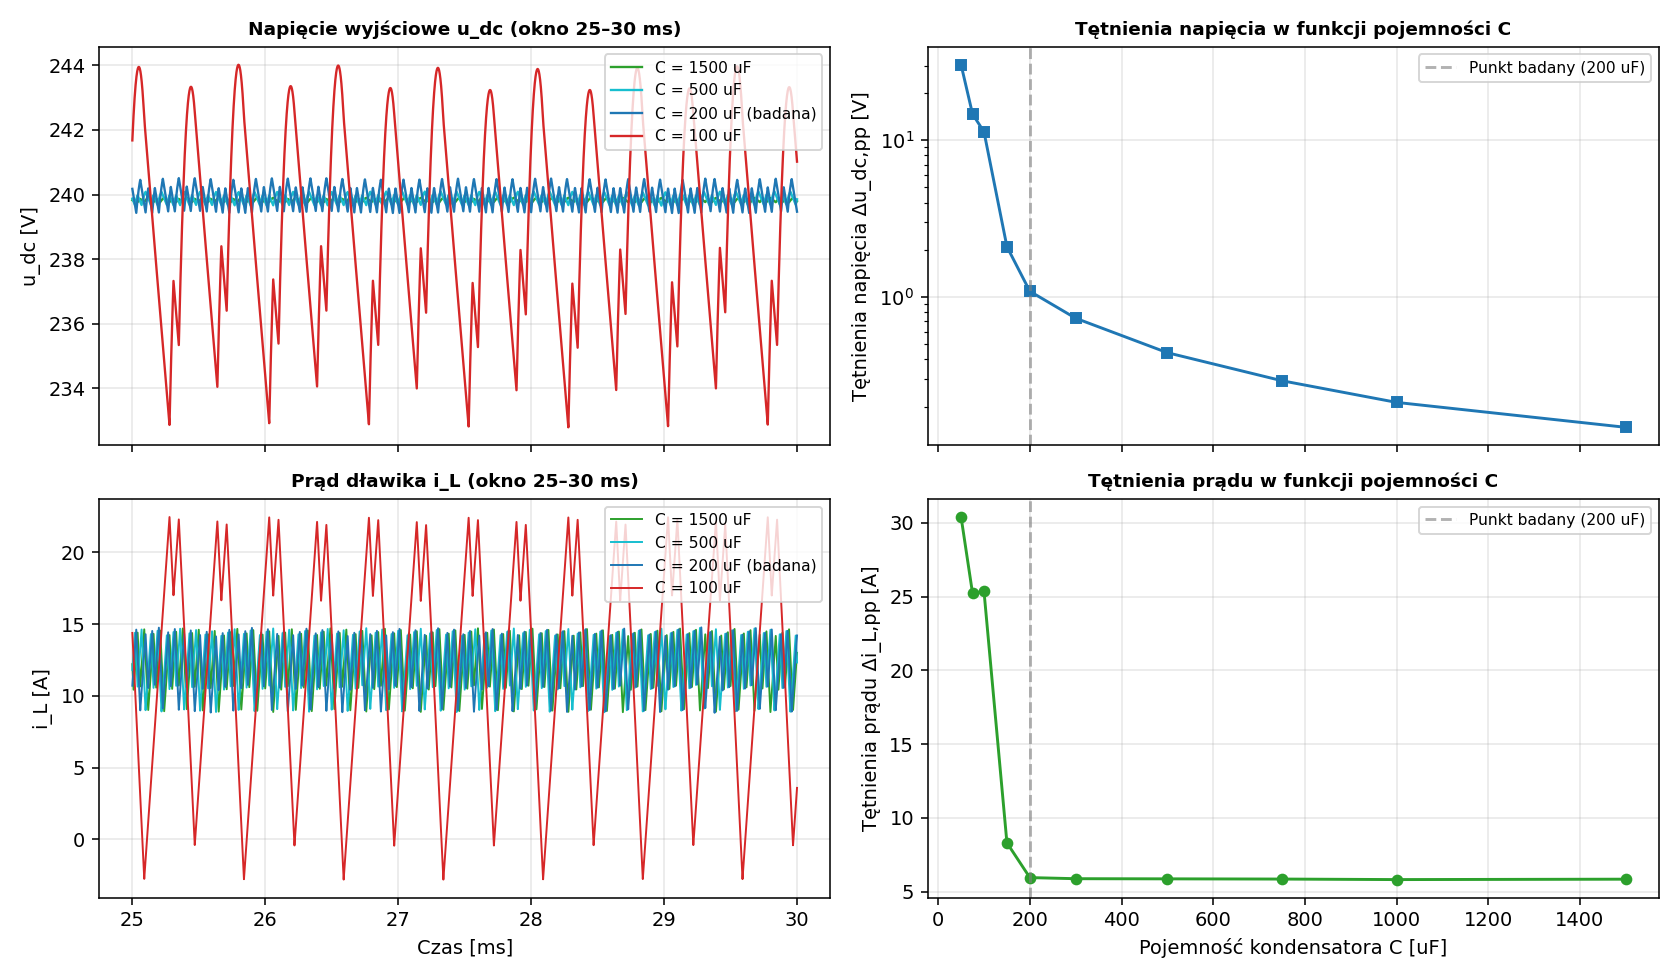
\includegraphics[width=\linewidth]{rysunki/stress_test_pojemnosci_c.png}
    \caption{Badanie zachowania przekształtnika przy redukcji pojemności wyjściowej $C$: (po lewej) przebiegi czasowe napięcia i~prądu w~stanie ustalonym; (po prawej) zależność tętnień napięcia $\Delta u_{\mathrm{dc},\mathrm{pp}}$ oraz tętnień prądu $\Delta i_{L,\mathrm{pp}}$ od pojemności $C$.}
    \label{fig:stress-c}
\end{figure}

Dla pojemności $C \ge 200~\mu\mathrm{F}$ układ zachowuje pełną stabilność, a~tętnienia prądu dławika pozostają na minimalnym poziomie sprzętowym ($\approx 5{,}85$--$5{,}96~\mathrm{A}$). Dla badanej w~pracy pojemności $C = 200~\mu\mathrm{F}$ tętnienia napięcia wynoszą zaledwie $1{,}09~\mathrm{V}$ ($0{,}45\,\%$), co stanowi wynik znakomity. Dopiero zejście poniżej $100~\mu\mathrm{F}$ przy taktowaniu $100~\mathrm{kHz}$ powoduje gwałtowny wzrost tętnień wskutek ograniczeń częstotliwości próbkowania sterownika.

\subsection{Odpowiedź dynamiczna na skoki obciążenia i~referencji}
\label{subsec:transient}

Odporność dynamiczną układu zweryfikowano w~horyzoncie $0{,}30~\mathrm{s}$ w~scenariuszu obejmującym skokowe zrzucenia obciążenia do stanu jałowego ($47{,}619~\Omega \to 10~\mathrm{M}\Omega$ w~$t=50~\mathrm{ms}$ i~$t=200~\mathrm{ms}$), ponowne dołączenia odbiornika $1{,}2~\mathrm{kW}$ ($t=100~\mathrm{ms}$ i~$t=250~\mathrm{ms}$) oraz skok wartości zadanej napięcia $240 \to 160~\mathrm{V}$ ($t=150~\mathrm{ms}$).

We wszystkich stanach przejściowych układ zachował stabilność:
\begin{itemize}
    \item Przy nagłym załączeniu pełnego obciążenia w~$t=100~\mathrm{ms}$ przeregulowanie napięcia wyniosło zaledwie $\Delta U_{\mathrm{overshoot}} = 0{,}51~\mathrm{V}$ ($0{,}21\,\%$ wartości zadanej).
    \item W~całym horyzoncie $0{,}30~\mathrm{s}$ prąd dławika nie przekroczył poziomu $22{,}63~\mathrm{A}$, co potwierdza skuteczne działanie ogranicznika nadprądowego ($I_{\max} = \pm 20~\mathrm{A}$).
    \item Zidentyfikowano jednak kluczowy problem dynamiczny: przy skoku referencji w~dół $240 \to 160~\mathrm{V}$ w~klasycznym sterowniku bez członu trendu występuje głęboki zapad napięcia poniżej zadanej wartości ($\sim 7$--$8~\mathrm{V}$), co motywuje konieczność zastosowania zautomatyzowanej optymalizacji metaheurystycznej i~rozbudowy algorytmu sterowania w~rozdziale~\ref{ch:ai}.
\end{itemize}

	\chapter{Zastosowanie sztucznej inteligencji w~optymalizacji sterowania}
\label{ch:ai}

% Rozdział 4 wg konspektu — integracja silnika DT z~algorytmem PSO. Matematyka
% roju, funkcja kosztu, automatyczna ewaluacja parametrów MF-BB, złożoność
% obliczeniowa i~zrównoleglanie.

\section{Wprowadzenie do metaheurystyk w~strojeniu sterowników}
\label{sec:metaheurystyki}

Klasyczne techniki strojenia regulatorów cyfrowych (metoda Zieglera-Nicholsa, lokowanie biegunów, kompensacja częstotliwościowa) zakładają znajomość zlinearyzowanego modelu obiektu sterowania w~okolicy wybranego punktu pracy. Założenie to staje się trudne do utrzymania w~przypadku silnie nieliniowych przekształtników kluczowanych, których dynamika zmienia się topologicznie wraz ze~stanem klucza półprzewodnikowego ($s\in\{0,1\}$), a~dodatkowy stopień złożoności wprowadza obecność członu predykcyjnego oraz cyfrowego filtru dolnoprzepustowego wewnątrz pętli sprzężenia zwrotnego. W~takiej sytuacji racjonalnym podejściem jest sformułowanie problemu jako numerycznej optymalizacji niedyferencjowalnej, w~której funkcja celu jest wartością skalarną wyznaczaną z~kompletnej symulacji bliźniaka cyfrowego dla zadanego wektora hiperparametrów regulatora~\cite{yang2014}.

W~rodzinie metaheurystyk rozważano trzy najpopularniejsze warianty: algorytmy genetyczne~(GA), symulowane wyżarzanie~(SA) oraz optymalizację rojem cząstek~(PSO). Spośród nich wybrano algorytm PSO, kierując się następującymi przesłankami:
\begin{enumerate}
    \item \textbf{Niska liczba hiperparametrów} -- kanoniczne PSO wymaga doboru jedynie trzech wartości (waga bezwładności $w$, współczynniki uczenia $c_1$, $c_2$), podczas gdy GA wymaga zdefiniowania operatorów selekcji, krzyżowania i~mutacji oraz ich prawdopodobieństw.
    \item \textbf{Naturalna ciągłość przestrzeni przeszukiwań} -- parametry regulatora MF-BB ($w_i\in\mathbb{R}_{+}$, $f_c\in\mathbb{R}_{+}$) są zmiennymi rzeczywistoliczbowymi, dla których binarna reprezentacja chromosomu w~GA byłaby sztuczna.
    \item \textbf{Dowiedziona skuteczność w~strojeniu regulatorów energoelektronicznych} -- w~literaturze tematu PSO występuje jako standardowe narzędzie strojenia układów PI/PID dla przekształtników DC-DC.
    \item \textbf{Trywialna paralelizacja} -- każda z~$N$ cząstek roju jest ewaluowana niezależnie, co~pozwala na~rozproszenie obciążenia obliczeniowego pomiędzy~dostępne rdzenie procesora.
\end{enumerate}

\section{Algorytm Optymalizacji Rojem Cząstek (PSO)}
\label{sec:pso}

\subsection{Podstawy matematyczne i~implementacja w~PySwarms}
\label{subsec:pso-math}

Algorytm optymalizacji rojem cząstek (ang.~\emph{Particle Swarm Optimization}, PSO) został zaproponowany przez Kennedy'ego i~Eberharta w~1995~roku~\cite{kennedy1995pso} jako stochastyczna metoda poszukiwania ekstremum w~wielowymiarowych przestrzeniach ciągłych, inspirowana zachowaniami społecznymi w~stadach ptaków oraz ławicach ryb. W~niniejszej pracy do~realizacji obliczeń optymalizacyjnych wykorzystano oficjalną bibliotekę naukową \texttt{PySwarms}~\cite{miranda2018pyswarms} (\texttt{pyswarms.single.GlobalBestPSO}), stanowiącą uznany w~literaturze akademickiej standard implementacyjny algorytmu roju w~języku Python.

W~algorytmie populacja $N$ cząstek przemieszcza się w~$d$-wymiarowej przestrzeni poszukiwań. Każda cząstka $i\in\{1,\dots,N\}$ w~kroku iteracyjnym $k$ jest opisana wektorem położenia $\mathbf{x}_i^{(k)}\in\mathbb{R}^d$ oraz wektorem prędkości $\mathbf{v}_i^{(k)}\in\mathbb{R}^d$. Cząstki wymieniają informację o~najlepszych dotychczasowych punktach: każda pamięta swoje najlepsze położenie indywidualne $\mathbf{p}_i$ (\emph{personal best}), a~cały rój utrzymuje pozycję najlepszą w~skali globalnej $\mathbf{g}$ (\emph{global best}). Zgodnie z~kanonicznym sformułowaniem biblioteki \texttt{PySwarms}, aktualizacja prędkości oraz położenia cząstek w~każdej iteracji przebiega według równań:
\begin{equation}
    \mathbf{v}_i^{(k+1)} = w^{(k)}\,\mathbf{v}_i^{(k)}
        + c_1\,r_1\odot\bigl(\mathbf{p}_i - \mathbf{x}_i^{(k)}\bigr)
        + c_2\,r_2\odot\bigl(\mathbf{g} - \mathbf{x}_i^{(k)}\bigr),
    \label{eq:pso-velocity}
\end{equation}
\begin{equation}
    \mathbf{x}_i^{(k+1)} = \mathbf{x}_i^{(k)} + \mathbf{v}_i^{(k+1)},
    \label{eq:pso-position}
\end{equation}
gdzie $r_1, r_2\sim\mathcal{U}([0,1]^d)$ są wektorami liczb losowych o~rozkładzie jednostajnym próbkowanymi niezależnie w~każdej iteracji, symbol $\odot$ oznacza iloczyn po~współrzędnych (Hadamarda), $c_1$ jest współczynnikiem przyciągania do~rekordu własnego (składnik kognitywny), $c_2$~--~współczynnikiem przyciągania do~rekordu roju (składnik społeczny), natomiast $w^{(k)}$ jest wagą bezwładności (ang.~\emph{inertia weight}).

Dla zachowania właściwego balansu pomiędzy globalną eksploracją przestrzeni na~początku procesu a~dokładną lokalną eksploatacją w~końcowych iteracjach, w~konfiguracji biblioteki \texttt{PySwarms} włączono strategię liniowej dekrementacji wagi bezwładności (\texttt{OptionsHandler.lin\_variation}) zgodnie z~metodyką Shi i~Eberharta~\cite{shi1998pso}:
\begin{equation}
    w^{(k)} = w_{\max} - \frac{k}{K_{\max}}\,(w_{\max} - w_{\min}),
    \label{eq:pso-inertia}
\end{equation}
gdzie $K_{\max}$ oznacza całkowitą liczbę iteracji optymalizatora.

Obsługę warunków brzegowych w~przestrzeni poszukiwań zrealizowano z~wykorzystaniem modułu odbicia lustrzanego \texttt{BoundaryHandler(strategy="reflective")}. W~przypadku przekroczenia dopuszczalnej granicy dziedziny współrzędna cząstki jest odbijana do~wnętrza obszaru dopuszczalnego, co zapobiega ucieczce roju i~utracie różnorodności populacji.

\subsection{Hiperparametry i~konfiguracja roju}
\label{subsec:pso-config}

W~niniejszej pracy przyjęto klasyczne wartości hiperparametrów PSO, sprawdzone w~literaturze przedmiotu dla zadań optymalizacji ciągłej średniej skali. Pełne zestawienie zawiera tabela~\ref{tab:pso-hparams}.

\begin{table}[h!]
    \centering
    \caption{Konfiguracja algorytmu PSO przyjęta w~eksperymentach (biblioteka \texttt{PySwarms}).}
    \label{tab:pso-hparams}
    \begin{tabular}{lcl}
        \toprule
        \textbf{Hiperparametr / Opcja} & \textbf{Wartość} & \textbf{Uzasadnienie} \\
        \midrule
        Środowisko obliczeniowe      & \texttt{PySwarms 1.3} & zweryfikowana biblioteka naukowa \\
        Topologia roju               & \texttt{Star} (globalna) & klasyczne $g_{\mathrm{best}}$ PSO \\
        Strategia brzegowa           & \texttt{reflective}  & odbicie lustrzane od granic \\
        Liczba cząstek $N$           & 16--20    & kompromis: koszt vs. pokrycie 2D \\
        Maks. liczba iteracji $K_{\max}$ & 25--40 & zbieżność do stabilnego plateau \\
        Waga bezwładności $w_{\max}$ & 0{,}9     & szeroka eksploracja na~starcie \\
        Waga bezwładności $w_{\min}$ & 0{,}4     & lokalna eksploatacja na~końcu \\
        Współczynnik kognitywny $c_1$ & 1{,}50--2{,}05 & standardowa waga pamięci własnej \\
        Współczynnik socjalny $c_2$  & 1{,}50--2{,}05 & standardowa waga pamięci roju \\
        Ziarno generatora $\texttt{seed}$ & 42   & pełna powtarzalność eksperymentu \\
        \bottomrule
    \end{tabular}
\end{table}

W~rozważanym zadaniu wymiar przestrzeni przeszukiwań wynosi $d=2$ (wektor $\mathbf{x}=[w_i,\,f_c]^\top$). Z~uwagi na~kilkurzędowy rozrzut wartości obu parametrów ($w_i\in[0{,}1;\,5]$ oraz $f_c\in[200;\,10\,000]$~Hz), całość optymalizacji prowadzona jest w~skali logarytmicznej -- cząstki operują w~przestrzeni $[\log_{10} x_{\min}, \log_{10} x_{\max}]^2$, a~przed wywołaniem funkcji celu wartości są transformowane potęgowo. Zabieg ten zapewnia równoważne pokrycie obu rzędów wielkości w~każdej z~dziedzin oraz zapobiega numerycznej dominacji jednej współrzędnej nad~drugą w~równaniu~\eqref{eq:pso-velocity}.

Jako warunek stopu przyjęto wyłącznie wyczerpanie maksymalnej liczby iteracji $K_{\max}=40$. Zrezygnowano z~kryterium stagnacji (brak~poprawy $\mathbf{g}$ przez $\Delta k$~iteracji), gdyż~przy~ustalonym małym budżecie ewaluacji nie wnosi ono istotnego skrócenia czasu, a~komplikuje analizę zbieżności prezentowaną w~rozdziale~\ref{sec:wyniki-pso}.

\section{Funkcje celu w~procesie strojenia}
\label{sec:fitness}

Wybór funkcji celu w~automatycznym strojeniu regulatora jest~decyzją programistyczną o~kluczowym znaczeniu dla~końcowego zachowania całego układu. Ten~sam algorytm PSO prowadzony identycznym budżetem obliczeniowym dla~odmiennych kryteriów jakości zwraca jakościowo różne nastawy regulatora -- jedne minimalizujące przeregulowanie kosztem dłuższego czasu ustalania, inne wymuszające szybką odpowiedź z~większymi tętnieniami prądu.

W~ramach badań zaimplementowano moduł \texttt{optymalizacja/cost\_functions.py}, w~którym zdefiniowano dwie komplementarne grupy kryteriów jakościowych:
\begin{enumerate}
    \item \textbf{Kryteria oparte na~błędzie napięcia:} oceniające wyłącznie jakość śledzenia zadanego napięcia wyjściowego $e_u(t) = u_{\mathrm{ref}}(t) - u_{dc}(t)$;
    \item \textbf{Kryteria świadome dynamiki prądu (ang.~\emph{current-aware}):} łączące minimalizację błędu napięcia z~penalizacją niepożądanych zjawisk w~dławiku (tętnień łączeniowych, oscylacji oraz nadmiernego prądu cewki).
\end{enumerate}

Wszystkie funkcje celu przyjmują jednolitą sygnaturę argumentów: wektory przebiegów $(t,\,u_{dc},\,i_L,\,s)$ uzyskane z~pojedynczej kompletnej symulacji, tablicę napięcia zadanego $u_{\mathrm{ref}}(t)$ oraz (w~przypadku kryteriów prądowych) wektor referencji prądu cewki $i_{\mathrm{des}}(t)$.

\subsection{Kryteria całkowe błędu napięcia: MSE, IAE, ITAE}
\label{subsec:cost-integral}

Trzy~pierwsze funkcje należą do~rodziny klasycznych kryteriów całkowych jakości regulacji:
\begin{equation}
    \begin{aligned}
        J_{\mathrm{MSE}}  &= \frac{1}{T}\int_0^{T} e_u^{2}(\tau)\,\mathrm{d}\tau, \\
        J_{\mathrm{IAE}}  &= \int_0^{T} \lvert e_u(\tau)\rvert\,\mathrm{d}\tau, \\
        J_{\mathrm{ITAE}} &= \int_0^{T} \tau\,\lvert e_u(\tau)\rvert\,\mathrm{d}\tau,
    \end{aligned}
    \label{eq:cost-integral}
\end{equation}
gdzie $T$~jest~horyzontem symulacji, a~$e_u(t) = u_{\mathrm{ref}}(t) - u_{dc}(t)$ oznacza chwilowy błąd regulacji napięcia. Numerycznie całki realizowane są~regułą trapezów (\texttt{numpy.trapezoid}) na~siatce czasowej pochodzącej bezpośrednio z~bliźniaka cyfrowego. Każde z~trzech kryteriów ma~odmienną charakterystykę: MSE silnie karze pojedyncze duże odchyłki (kara kwadratowa), IAE traktuje błędy liniowo w~całym horyzoncie, zaś ITAE poprzez~mnożnik czasu $\tau$ dodatkowo penalizuje błędy utrzymujące się pod~koniec horyzontu, co~skutecznie eliminuje powolne oscylacje w~stanie ustalonym.

\subsection{Kryterium asymetryczne}
\label{subsec:cost-asymmetric}

W~przekształtniku DC-DC zasilającym wrażliwe odbiorniki, przeregulowanie powyżej~$u_{\mathrm{ref}}$ jest~zjawiskiem znacznie bardziej niepożądanym niż~przejściowy spadek napięcia poniżej zadania -- grozi ono przebiciem izolacji lub~uszkodzeniem kondensatorów wyjściowych pracujących blisko swojego napięcia znamionowego. Aby~proces optymalizacji respektował tę~właściwość fizyczną, wprowadzono kryterium asymetryczne:
\begin{equation}
    J_{\mathrm{Asym}} = \int_0^{T} \Bigl[\lambda_{\mathrm{asym}}\,\bigl(\max(-e_u,0)\bigr)^{2}
        + \bigl(\max(e_u,0)\bigr)^{2}\Bigr]\,\mathrm{d}\tau,
    \label{eq:cost-asymmetric}
\end{equation}
gdzie współczynnik~$\lambda_{\mathrm{asym}} = 5$ pięciokrotnie zwiększa karę za~dodatnie przekroczenie napięcia ($u_{dc} > u_{\mathrm{ref}}$).

\subsection{Kryterium kompozytowe}
\label{subsec:cost-composite}

Kolejnym wariantem jest~kryterium kompozytowe łączące bezpośrednio trzy inżynierskie wskaźniki jakości odpowiedzi skokowej -- czas ustalania~$t_s$, przeregulowanie~$M_p$ oraz błąd ustalony~$e_{ss}$:
\begin{equation}
    J_{\mathrm{Comp}} = \alpha\,t_s + \beta\,M_p + \gamma\,e_{ss},
    \label{eq:cost-composite}
\end{equation}
przy~czym $t_s$~wyrażone jest~w~milisekundach (pasmo 2\,\% wartości zadanej), $M_p$~w~procentach napięcia zadanego, a~$e_{ss}$~w~woltach (średnia z~ostatnich 5\,\% przebiegu). Wagi $\alpha = 100$, $\beta = 10$, $\gamma = 50$ dobrano tak, aby~poszczególne składniki wnosiły porównywalny udział do~wartości skalarnej.

W~odróżnieniu od~kryteriów całkowych, kryterium kompozytowe wymaga uprzedniej dyskretyzacji przebiegu do~wskaźników skalarnego pasma, co~sprawia, że~powierzchnia kosztu jest~kawałkami stała i~niegładka. Skutkuje to~pogorszeniem zbieżności algorytmu PSO w~porównaniu z~kryteriami całkowymi.

\subsection{Kryteria uwzględniające dynamikę prądu cewki}
\label{subsec:cost-current}

Wstępne badania oparte wyłącznie na~błędzie napięcia wyjściowego ujawniły istotne ograniczenie: dążąc do~maksymalnego skrócenia czasu narastania napięcia, algorytm optymalizacyjny potrafi wybrać nastawy regulatora prowadzące do~patologicznie dużych tętnień prądu cewki (w~skrajnych punktach przestrzeni nastaw amplituda tętnień prądu $\Delta i_L$ przekraczała $25~\mathrm{A}$). Duże tętnienia prądu generują nadmiarowe straty komutacyjne w~tranzystorach, przeciążenia cieplne dławika oraz przenoszą się wprost na~tętnienia napięcia szyny DC.

W~celu wyeliminowania tego problemu sformułowano trzy dedykowane warianty funkcji celu penalizujące niepożądane składowe prądu dławika:

\begin{enumerate}
    \item \textbf{Wariant 1: CurrentAware (kara za~błąd śledzenia prądu).} Łączy całkowy błąd napięcia z~błędem śledzenia pożądanego prądu cewki $i_{\mathrm{des}}$:
    \begin{equation}
        J_{\mathrm{CA}} = J_{\mathrm{IAE},u} + \lambda_i \cdot \int_0^T \lvert i_{\mathrm{des}}(\tau) - i_L(\tau) \rvert\,\mathrm{d}\tau,
        \label{eq:cost-currentaware}
    \end{equation}
    gdzie waga $\lambda_i = 1{,}0$ równoważy rzędy wielkości obu całek. Wariant ten bezpośrednio nagradza sterownik za~zgodność chwilowego prądu z~jego średnim punktem pracy, ograniczając powstawanie zniekształceń prądowych w~stanach ustalonych.
    
    \item \textbf{Wariant 2: CurrentOscillation (kara za~lokalne wahania w~oknie próbek).} Aby~uniknąć penalizacji naturalnego, wymuszonego prawami fizyki narastania prądu w~momencie skoku napięcia zadanego, wprowadzono kryterium oparte na~przesuwnym oknie czasowym:
    \begin{equation}
        J_{\mathrm{CO}} = J_{\mathrm{IAE},u} + \mu_{\mathrm{osc}} \cdot \frac{1}{M}\sum_{m=1}^M \Bigl(\max_{k\in W_m} i_L[k] - \min_{k\in W_m} i_L[k]\Bigr)^2,
        \label{eq:cost-currentoscillation}
    \end{equation}
    gdzie $W_m$ oznacza okno $W = 4$ kolejnych próbek prądu rejestrowanych w~takcie sterownika ($T_s = 10~\mu\mathrm{s}$), a~$\mu_{\mathrm{osc}} = 0{,}02$. Rozstęp (różnica maksimum i~minimum) w~krótkim oknie $40~\mu\mathrm{s}$ jest~prawie niewrażliwy na~wolne narastanie prądu średniego, natomiast silnie karze szybkie oscylacje międzypróbkowe.
    
    \item \textbf{Wariant 3: CurrentEffort (kara za~energię prądu).} Penalizuje kwadrat prądu dławika (odpowiednik członu \emph{control effort} znanego z~regulatorów LQR):
    \begin{equation}
        J_{\mathrm{CE}} = J_{\mathrm{IAE},u} + \gamma_{\mathrm{eff}} \cdot \int_0^T i_L^2(\tau)\,\mathrm{d}\tau,
        \label{eq:cost-currenteffort}
    \end{equation}
    ze~współczynnikiem $\gamma_{\mathrm{eff}} = 0{,}02$. Wariant ten wprowadzono jako kontrprzykład fizyczny: ponieważ prąd średni w~stanie ustalonym wynika bezpośrednio z~bilansu mocy $I_L = u_{dc}^2 / (R V_{\mathrm{in}})$, zbyt silne karanie samej amplitudy prądu wymusza na~optymalizatorze obniżanie napięcia wyjściowego poniżej wartości zadanej (trwały błąd ustalony).
\end{enumerate}

\section{Integracja PSO z~silnikiem fizycznym}
\label{sec:pso-integration}

Zaletą oddzielenia silnika fizycznego (rozdział~\ref{ch:realizacja}) od~warstwy strojenia jest~możliwość wpięcia algorytmu PSO bez~jakichkolwiek modyfikacji rdzenia symulacyjnego. Cały moduł optymalizacyjny (\texttt{optymalizacja/}) traktuje silnik jako funkcję typu \emph{black-box}, której pojedyncze wywołanie odpowiada jednej~ewaluacji funkcji celu dla~ustalonej pary $(w_i, f_c)$. Pętla optymalizacji składa się z~trzech logicznie wyodrębnionych komponentów: definicji scenariusza testowego, opcjonalnego baseline'u opartego o~grid search oraz właściwej pętli ewaluacji wywoływanej z~wnętrza PSO.

\subsection{Scenariusz testowy}
\label{subsec:pso-scenario}

Jakość strojenia regulatora ujawnia się dopiero w~obecności zaburzeń wymuszających aktywne przełączanie klucza półprzewodnikowego. Z~tego powodu wszystkie eksperymenty optymalizacyjne wykonano w~tzw.~\emph{scenariuszu trudnym} (\texttt{optymalizacja/scenarios.py}\,/\,\texttt{hard\_scenario}), w~którym horyzont $T = 200$~ms został podzielony na~cztery 50-milisekundowe odcinki:
\begin{enumerate}
    \item $t\in[0,\,50)$~ms -- rozruch z~$u_{dc}(0)=100$~V do~$u_{\mathrm{ref}}=240$~V przy~obciążeniu $R = 47{,}6~\Omega$;
    \item $t = 50$~ms -- skokowe \emph{odciążenie} $R \leftarrow 95{,}238~\Omega$ (obciążenie redukowane do~połowy mocy), wymuszające szybkie zdławienie nadwyżki energii w~kondensatorze przez~regulator ($s = 0$);
    \item $t\in(50,\,100)$~ms -- stan ustalony przy~zmniejszonym obciążeniu;
    \item $t = 100$~ms -- skok zadania $u_{\mathrm{ref}} \leftarrow 260$~V, wymagający aktywnego pchnięcia prądu cewki z~zachowaniem ograniczenia $i_L < i_{\max} = 20$~A.
\end{enumerate}
Powyższa konfiguracja została dobrana eksperymentalnie po~odrzuceniu wcześniejszego wariantu z~\emph{dociążeniem} ($R/2$) i~skokiem zadania w~dół, w~którym nastawy regulatora okazały się nie~mieć wpływu na~przebieg -- dociążenie aktywowało zabezpieczenie nadprądowe (OCP), a~skok w~dół powodował pasywne rozładowanie kondensatora przez~odbiornik. W~obecnym wariancie obie operacje (odciążenie + ref-step w~górę) wymagają jawnego sterowania kluczem, co~różnicuje funkcję kosztu względem nastaw $(w_i, f_c)$. Reprezentatywne przebiegi scenariusza dla~jednego punktu pracy zilustrowano na~rysunku~\ref{fig:scenario-check}.

\begin{figure}[h!]
    \centering
    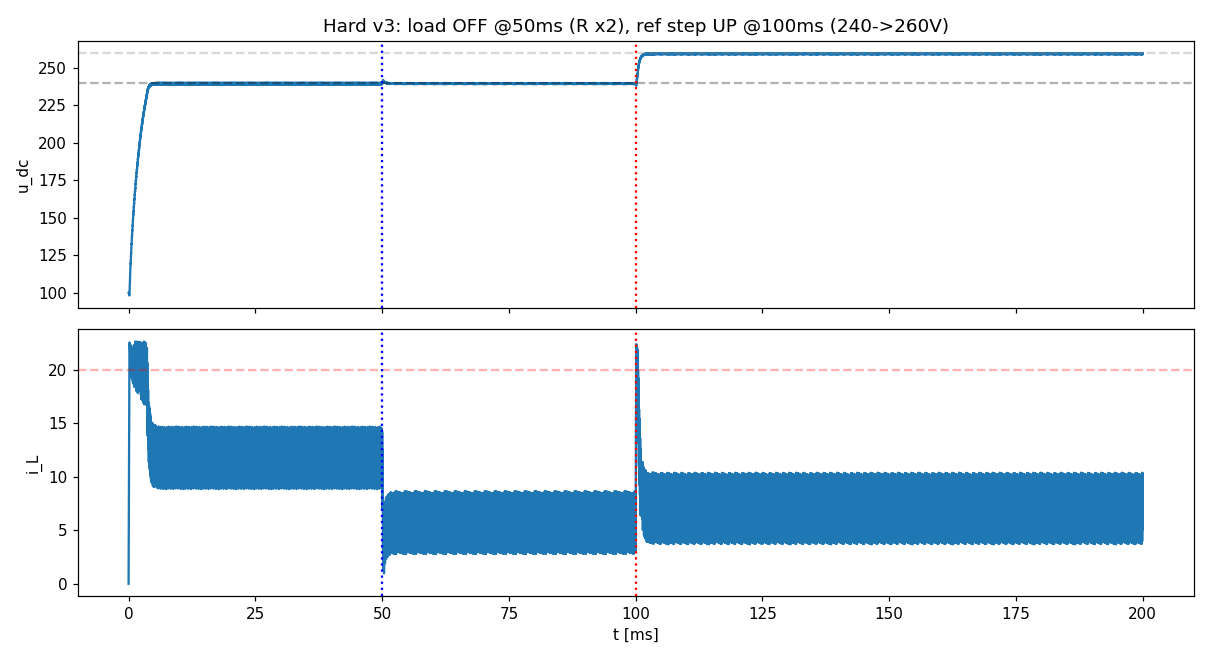
\includegraphics[width=0.95\linewidth]{rysunki/scenario_check.png}
    \caption{Weryfikacja scenariusza trudnego: przebieg napięcia $u_{dc}(t)$ i~prądu cewki $i_L(t)$ dla~ustalonej pary nastaw regulatora. Widoczne dwa zdarzenia: skokowe odciążenie w~$t = 50$~ms oraz skok zadania $240 \to 260$~V w~$t = 100$~ms.}
    \label{fig:scenario-check}
\end{figure}

\subsection{Baseline siatkowy (grid search 15$\times$15)}
\label{subsec:pso-grid}

Przed~uruchomieniem właściwej optymalizacji rojem cząstek przeprowadzono pełną ewaluację siatkową w~przestrzeni $(w_i, f_c)$ na~kracie $15\times 15 = 225$~węzłów, rozmieszczonych równomiernie w~skali logarytmicznej (\texttt{optymalizacja/grid\_search.py}). Granice siatki przyjęto analogicznie do~granic przestrzeni PSO ($w_i\in[0{,}1;\,5]$, $f_c\in[200;\,10\,000]$~Hz). Dla~każdego z~225 węzłów wykonano kompletną symulację scenariusza trudnego oraz~obliczono wszystkie pięć funkcji celu zdefiniowanych w~podrozdziale~\ref{sec:fitness}, otrzymując w~rezultacie pięć dwuwymiarowych map kosztu zobrazowanych na~rysunku~\ref{fig:mapy-kosztow}.

\begin{figure}[h!]
    \centering
    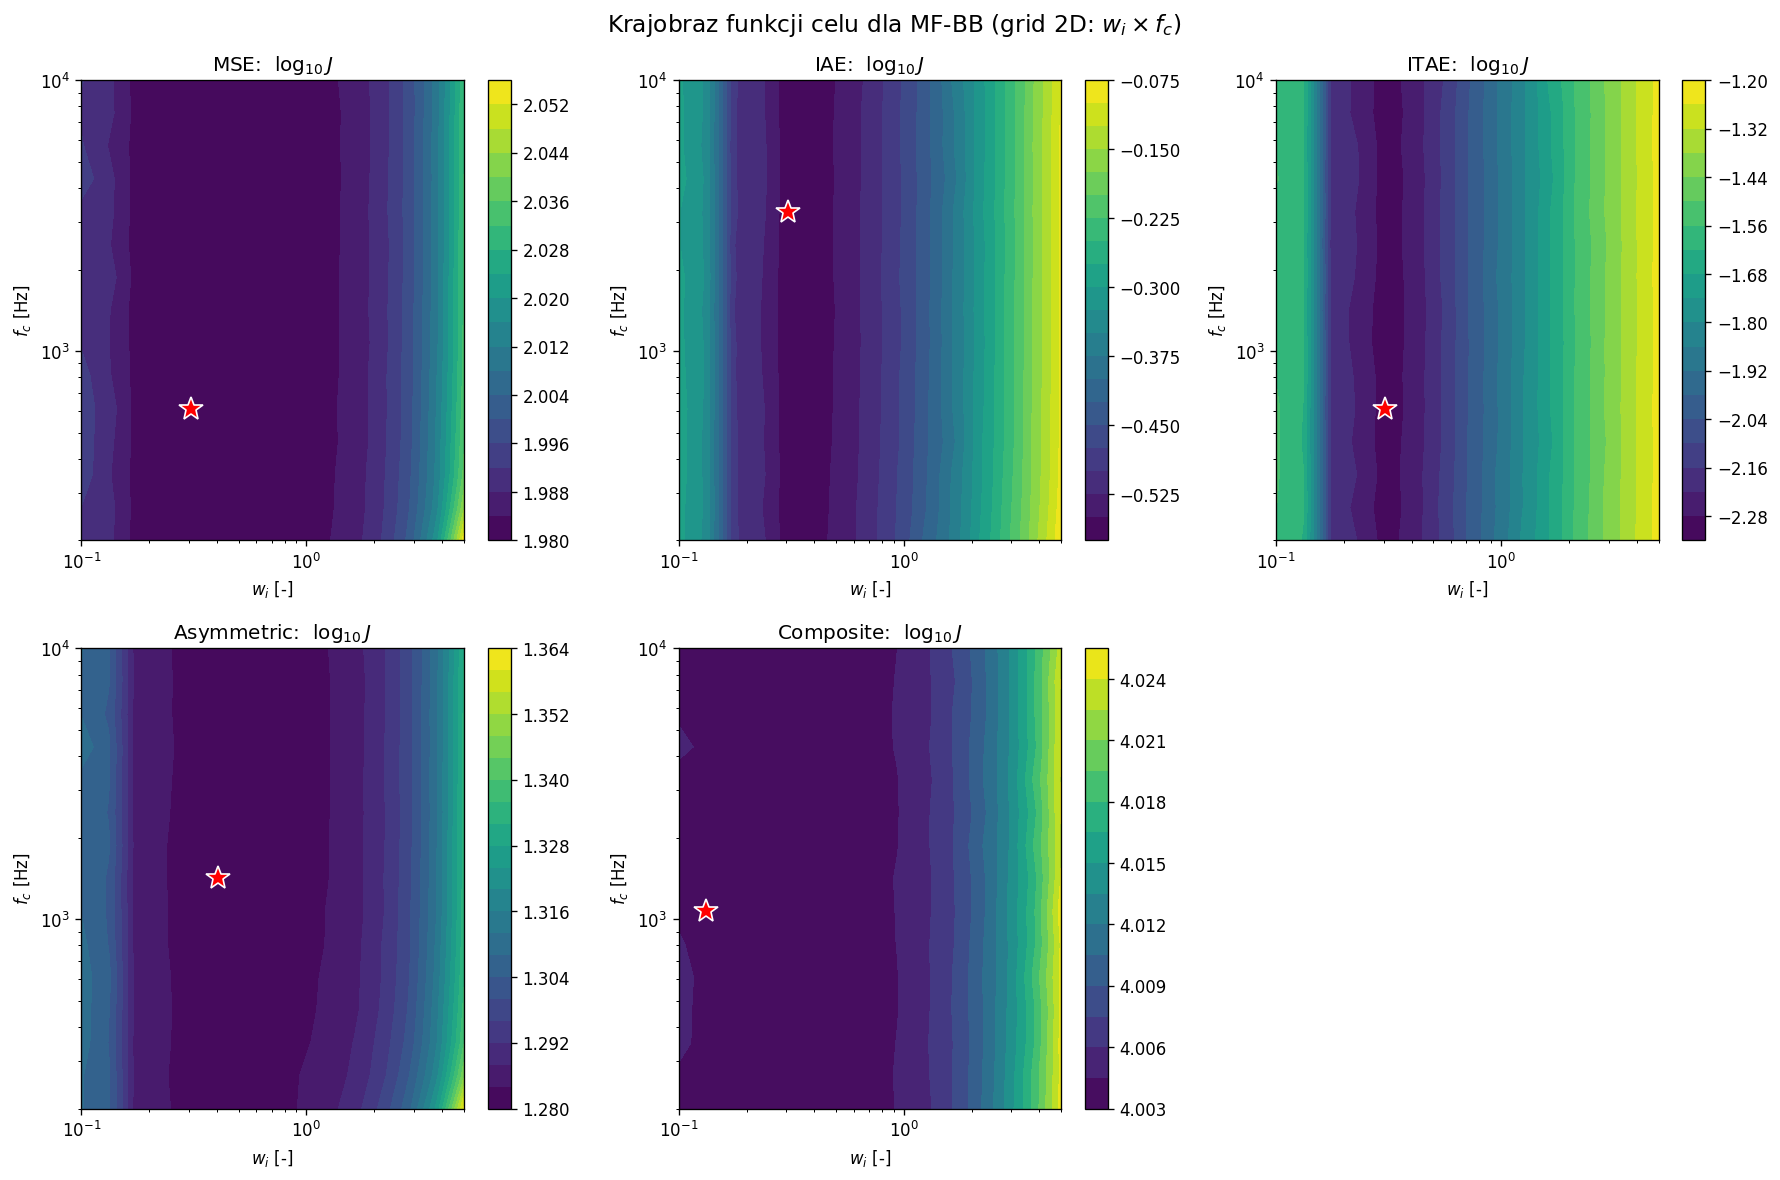
\includegraphics[width=\linewidth]{rysunki/mapy_kosztow.png}
    \caption{Mapy funkcji kosztu w~przestrzeni $(w_i, f_c)$ uzyskane z~grid searcha $15\times 15$ węzłów. Każda mapa odpowiada jednej z~pięciu funkcji celu (MSE, IAE, ITAE, asymetryczna, kompozytowa). Skala logarytmiczna na~obu osiach, krzyżyk oznacza minimum globalne~siatki.}
    \label{fig:mapy-kosztow}
\end{figure}

Baseline siatkowy pełni dwie funkcje. Po~pierwsze, dostarcza punktu odniesienia (\emph{ground truth} w~granicach rozdzielczości kraty) względem~którego można ocenić skuteczność PSO -- algorytm metaheurystyczny powinien znaleźć rozwiązanie nie~gorsze od~najlepszego węzła siatki, zazwyczaj jednak lepsze, gdyż~działa w~przestrzeni ciągłej. Po~drugie, mapy kosztu ujawniają jakościowy charakter krajobrazu optymalizacyjnego -- obecność wielu minimów lokalnych, długich dolin oraz~obszarów płaskich, co~bezpośrednio uzasadnia konieczność użycia metody globalnej zamiast~klasycznych gradientowych. Przebiegi czasowe odpowiadające nastawom optymalnym dla~każdej z~pięciu funkcji celu zestawiono na~rysunku~\ref{fig:przebiegi-optimum}.

\begin{figure}[h!]
    \centering
    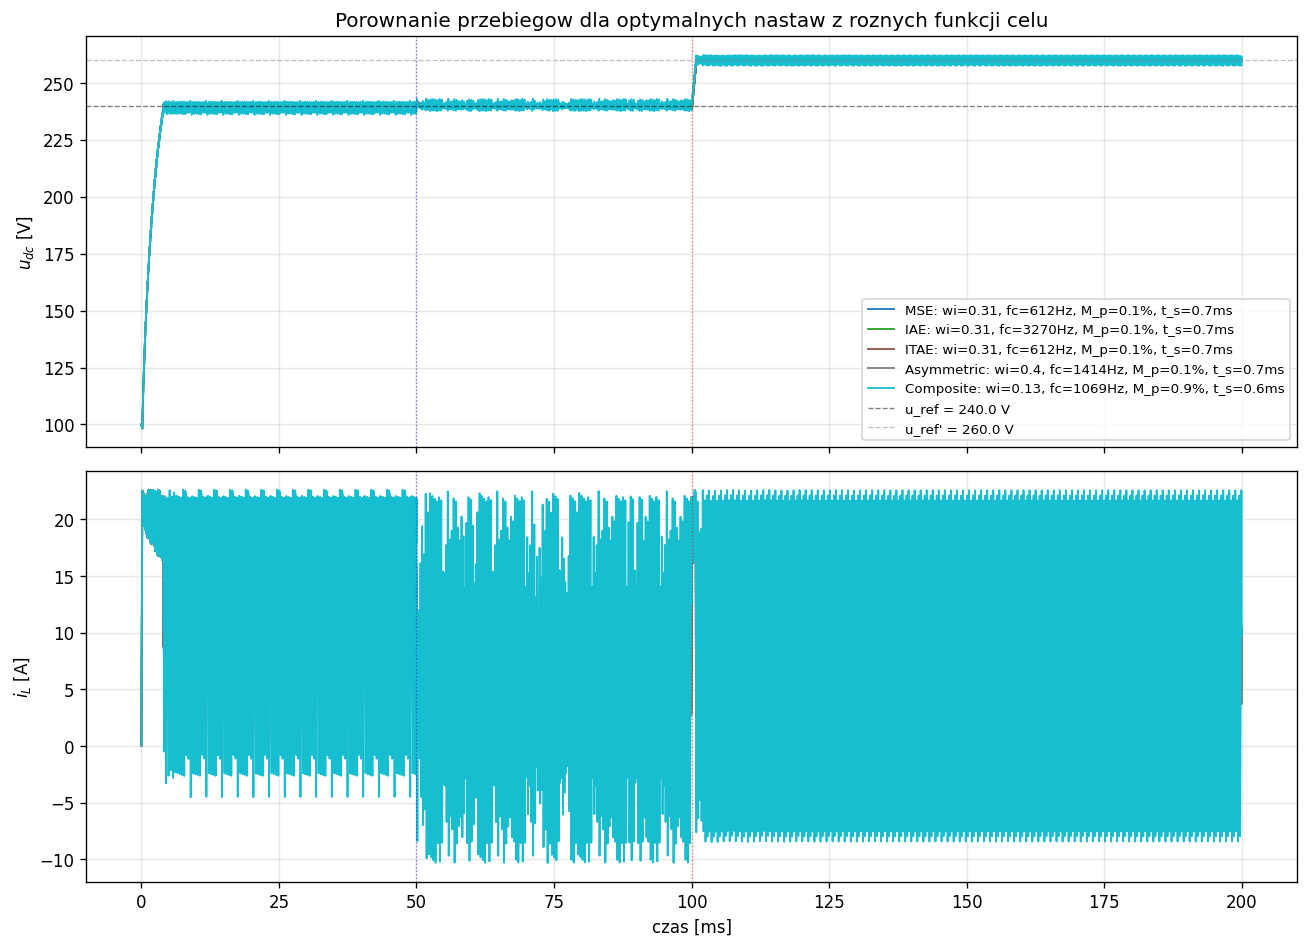
\includegraphics[width=\linewidth]{rysunki/przebiegi_optimum.png}
    \caption{Przebiegi napięcia $u_{dc}(t)$ uzyskane dla~nastaw $(w_i^*,f_c^*)$ minimalizujących każdą z~pięciu funkcji celu na~siatce $15\times 15$. Widoczne jakościowe różnice odpowiedzi -- kryteria całkowe (MSE/IAE/ITAE) faworyzują szybką, agresywną dynamikę, natomiast kryterium asymetryczne i~kompozytowe prowadzą do~odpowiedzi bardziej zachowawczych.}
    \label{fig:przebiegi-optimum}
\end{figure}

\subsection{Pętla ewaluacji w~PSO}
\label{subsec:pso-loop}

Właściwa pętla strojenia jest~realizowana przez~funkcję \texttt{evaluate(log\_wi, log\_fc, cost\_name)} z~modułu \texttt{optymalizacja/pso.py}, której kolejne wywołania PSO wykonuje wewnątrz pętli głównej dla~każdej cząstki w~każdej iteracji. Algorytmiczne kroki pojedynczej ewaluacji są~następujące:
\begin{enumerate}
    \item potęgowanie współrzędnych cząstki: $w_i \leftarrow 10^{\log w_i}$, $f_c \leftarrow 10^{\log f_c}$ (przejście z~przestrzeni PSO do~przestrzeni fizycznej);
    \item podmiana nastaw regulatora w~kopii konfiguracji domyślnej (\texttt{default\_config()}) z~jednoczesnym podpięciem scenariusza trudnego i~horyzontu $T = 200$~ms;
    \item wywołanie metody \texttt{Simulator(cfg).run()} -- pełna symulacja $\sim$$4\cdot 10^{5}$ kroków;
    \item zbudowanie tablicy zadania $u_{\mathrm{ref}}(t)$ uwzględniającej ref-step;
    \item wywołanie funkcji kosztu wybranej z~rejestru \texttt{COST\_FUNCTIONS} i~zwrócenie wartości skalarnej.
\end{enumerate}

Z~perspektywy PSO funkcja \texttt{evaluate} jest~deterministyczną odpowiednikiem czarnej skrzynki -- dla~tych samych argumentów zwraca tę~samą wartość (silnik fizyczny nie~używa generatorów liczb pseudolosowych, a~całe źródło stochastyczności sprowadza się do~inicjalizacji roju przez~\texttt{numpy.random.default\_rng(seed=42)}). Dzięki temu pojedyncze uruchomienie eksperymentu jest~w~pełni powtarzalne, co~ma~kluczowe znaczenie dla~odtwarzalności wyników raportowanych w~rozdziale~\ref{sec:wyniki-pso}.

\section{Wyniki strojenia PSO i~porównanie z~baseline'em}
\label{sec:wyniki-pso}

Algorytm PSO uruchomiono pięciokrotnie -- po~jednym przebiegu na~każdą z~funkcji celu zdefiniowanych w~podrozdziale~\ref{sec:fitness}, przy~tej samej konfiguracji hiperparametrów wymienionych w~tabeli~\ref{tab:pso-hparams} oraz tym samym ziarnie generatora pseudolosowego ($\texttt{seed}=42$). Łączny budżet ewaluacji wyniósł $N\cdot(K_{\max}+1) = 20\cdot 41 = 820$ wywołań silnika fizycznego (kolumna inicjalna~+~$K_{\max}$ iteracji aktualizacji). Wartości optymalnych nastaw $(w_i^*,\,f_c^*)$ wraz z~odpowiadającymi wartościami funkcji celu $J^*$ zestawiono w~tabeli~\ref{tab:pso-wyniki}.

\begin{table}[h!]
    \centering
    \caption{Optymalne nastawy regulatora MF-BB znalezione przez~PSO dla~pięciu funkcji celu (scenariusz trudny, $T = 200$~ms).}
    \label{tab:pso-wyniki}
    \begin{tabular}{lrrr}
        \toprule
        \textbf{Funkcja celu} & $w_i^*$ & $f_c^*$ [Hz] & $J^*$ \\
        \midrule
        MSE        & 0{,}288 & 9569 & $9{,}55\cdot 10^{1}$ \\
        IAE        & 0{,}283 & 2701 & $2{,}69\cdot 10^{-1}$ \\
        ITAE       & 0{,}276 & 9493 & $4{,}71\cdot 10^{-3}$ \\
        Asymetryczna & 0{,}395 & 6902 & $1{,}91\cdot 10^{1}$ \\
        Kompozytowa & 0{,}136 & \phantom{0}618 & $1{,}01\cdot 10^{4}$ \\
        \bottomrule
    \end{tabular}
\end{table}

Pierwsze obserwacje strukturalne dotyczą lokalizacji minimów w~przestrzeni nastaw. Cztery kryteria całkowe (MSE, IAE, ITAE, asymetryczne) wskazują podobny zakres wagi inercji $w_i^* \in [0{,}28;\,0{,}40]$, co~odpowiada umiarkowanej dynamice członu predykcyjnego. Wyróżnia się jedynie kryterium kompozytowe, dla~którego $w_i^* = 0{,}136$ jest~bliskie dolnej granicy przestrzeni przeszukiwań -- regulator preferuje wówczas niemal wyłącznie sygnał błędu, kosztem reakcji predykcyjnej, co~jest~bezpośrednią konsekwencją dominacji składnika $\alpha\cdot t_s$ w~funkcji $J_{\mathrm{Comp}}$ (równanie~\eqref{eq:cost-composite}). Częstotliwość filtru $f_c^*$ jest~znacznie bardziej rozproszona -- od~618~Hz (Composite) do~9569~Hz (MSE), co~odzwierciedla różnicę między~kryteriami penalizującymi pojedyncze szczyty (wymagają agresywnej filtracji, $f_c$~wysokie) a~kryteriami uśredniającymi (tolerują niższe pasmo).

Charakter zbieżności roju dla~poszczególnych funkcji celu pokazano na~rysunku~\ref{fig:pso-zbieznosc-porown}. Wszystkie pięć przebiegów osiągnęło stabilne plateau przed~upływem zadeklarowanego budżetu $K_{\max}=40$ iteracji (ITAE: iteracja~34, Composite: 28, pozostałe: 38--40), co~potwierdza wystarczalność przyjętej konfiguracji. Charakterystyczne stopniowe spadki w~początkowych iteracjach odpowiadają pierwszym odkryciom obszarów obiecujących przez~poszczególne cząstki, natomiast późniejsza monotoniczna zbieżność wynika z~liniowej dekrementacji wagi bezwładności (równanie~\eqref{eq:pso-inertia}).

\begin{figure}[h!]
    \centering
    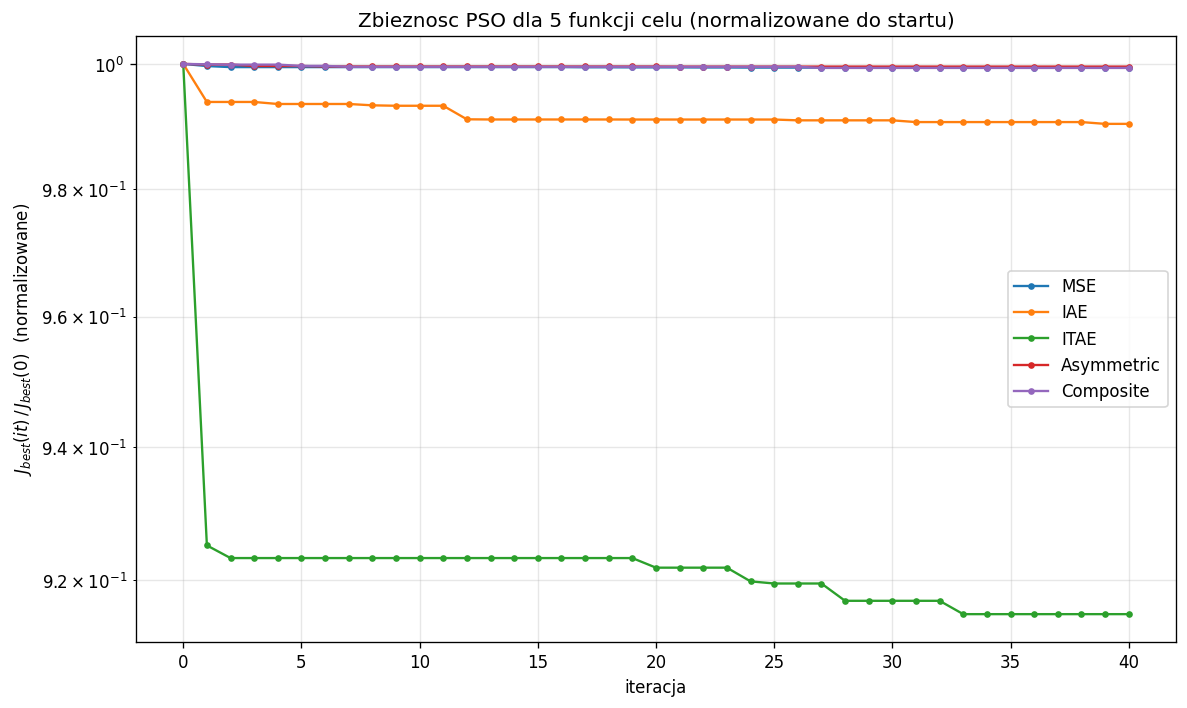
\includegraphics[width=\linewidth]{rysunki/pso_porownanie_zbieznosci.png}
    \caption{Krzywe zbieżności PSO dla~pięciu funkcji celu w~funkcji numeru iteracji. Każda krzywa znormalizowana do~swojej wartości początkowej ($J^{(0)}/J^{(0)}=1$); skala logarytmiczna podkreśla ostatnie rzędy poprawy.}
    \label{fig:pso-zbieznosc-porown}
\end{figure}

Wizualizację samego procesu przeszukiwania przedstawia rysunek~\ref{fig:pso-roj}, na~którym kolejne pozycje wszystkich cząstek roju zostały naniesione na~mapę funkcji kosztu uzyskaną z~grid searcha. Dla~każdej z~pięciu funkcji celu obserwuje się charakterystyczne kondensowanie się chmury cząstek wokół minimum w~ciągu pierwszych 10--15 iteracji, po~czym następuje faza dokładnej lokalnej eksploracji w~zwartym obszarze.

\begin{figure}[h!]
    \centering
    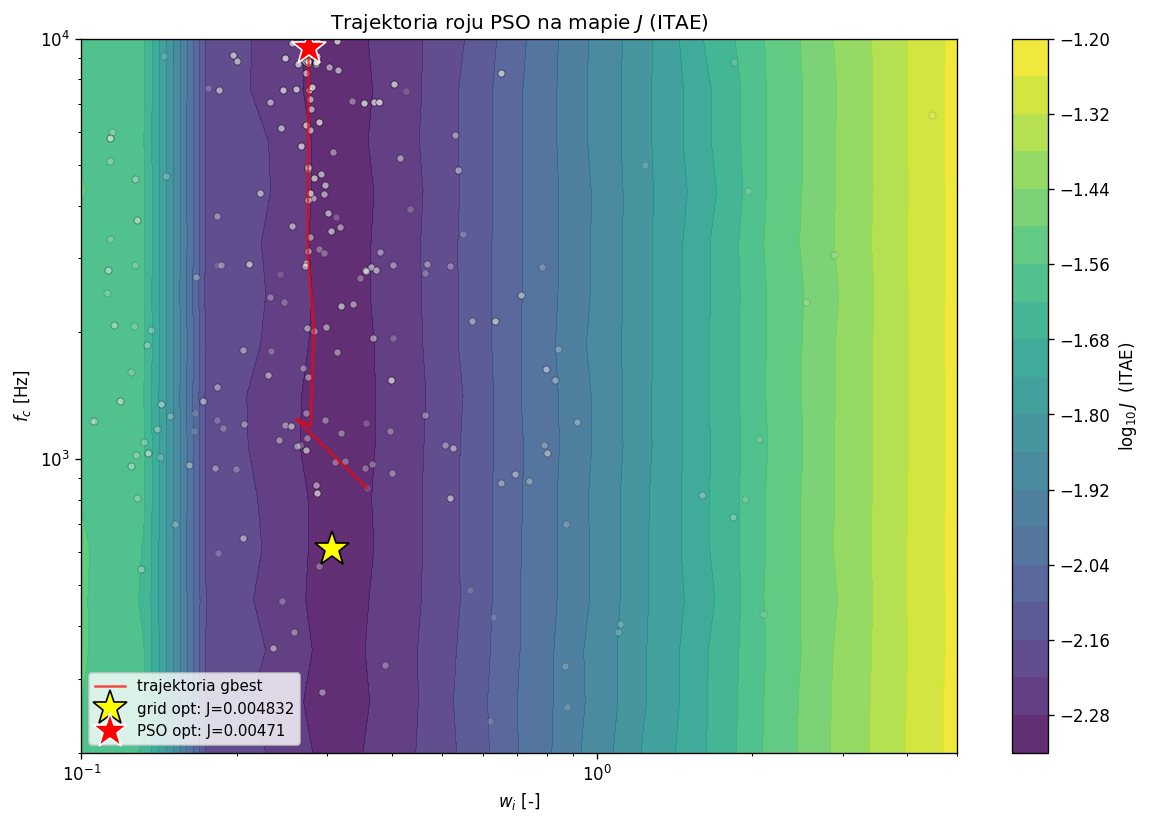
\includegraphics[width=\linewidth]{rysunki/pso_roj_na_mapie.png}
    \caption{Trajektoria roju cząstek PSO nałożona na~mapę funkcji kosztu (grid search 15$\times$15) dla~pięciu funkcji celu. Kolory cząstek odpowiadają numerowi iteracji (gradient od~jasnego do~ciemnego), gwiazda oznacza znalezione $\mathbf{g}^*$.}
    \label{fig:pso-roj}
\end{figure}

\subsection{Porównanie ilościowe PSO vs.~grid search}
\label{subsec:pso-vs-grid}

Bezpośrednie zestawienie wartości funkcji celu osiągniętych przez~PSO i~przez~najlepszy węzeł siatki bazowej (225~symulacji) przedstawia rysunek~\ref{fig:pso-vs-grid}. PSO uzyskuje wartości funkcji celu nie~gorsze od~baseline'u siatkowego dla~wszystkich pięciu kryteriów, przy~czym największą poprawę odnotowano dla~kryterium ITAE: wartość $J^*_{\mathrm{PSO}} = 4{,}71\cdot 10^{-3}$ jest~o~ok.~2{,}5\% niższa od~minimum siatkowego $J^*_{\mathrm{grid}} = 4{,}83\cdot 10^{-3}$. Dla~pozostałych kryteriów różnica jest~marginalna (poniżej~0{,}3\%), co~należy interpretować jako~potwierdzenie, że~siatka 15$\times$15 trafiła blisko prawdziwego optimum, a~PSO dokończył eksplorację w~przestrzeni ciągłej.

\begin{figure}[h!]
    \centering
    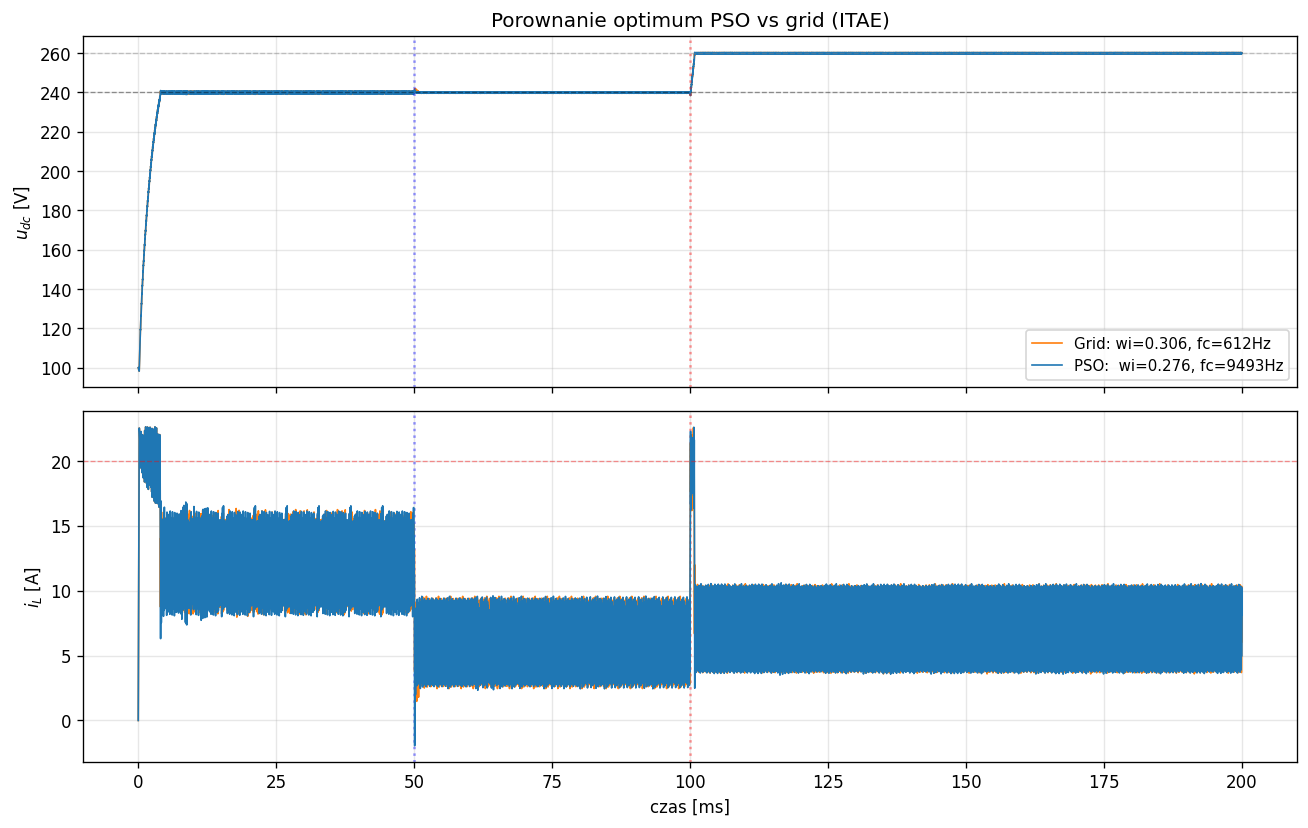
\includegraphics[width=0.85\linewidth]{rysunki/pso_vs_grid.png}
    \caption{Porównanie wartości funkcji celu $J^*$ uzyskanej przez~PSO (820~ewaluacji) z~minimum siatki 15$\times$15 (225~ewaluacji) dla~pięciu kryteriów. Wartości znormalizowane do~minimum grid (=1{,}00); PSO poniżej~1 oznacza lepszy wynik.}
    \label{fig:pso-vs-grid}
\end{figure}

Z~perspektywy efektywności obliczeniowej PSO osiągnął porównywalne wyniki przy~3,6-krotnie większej liczbie ewaluacji (820 vs.~225). Przewaga metaheurystyki ujawnia się jednak dopiero przy~rozszerzeniu wymiaru przestrzeni przeszukiwań -- dla~regulatora z~$d=4$ hiperparametrami (np.~dodanie współczynników predyktora) siatka tej~samej rozdzielczości wymagałaby $15^4 = 50\,625$ symulacji, podczas gdy PSO zachowuje liniową złożoność $\mathcal{O}(N\cdot K_{\max})$ niezależnie od~$d$.

Jakościowe porównanie wpływu wyboru funkcji celu na~odpowiedź czasową regulatora przedstawia rysunek~\ref{fig:pso-przebiegi}. Widoczne są~istotne różnice charakteru regulacji: kryterium kompozytowe prowadzi do~zauważalnego undershoot po~skoku zadania (skutek dominacji $\alpha\cdot t_s$), kryterium asymetryczne praktycznie eliminuje przeregulowanie kosztem dłuższego czasu ustalania, natomiast kryteria MSE/IAE/ITAE generują odpowiedzi zbliżone jakościowo, z~niewielkim przeregulowaniem rzędu kilku~procent.

\begin{figure}[h!]
    \centering
    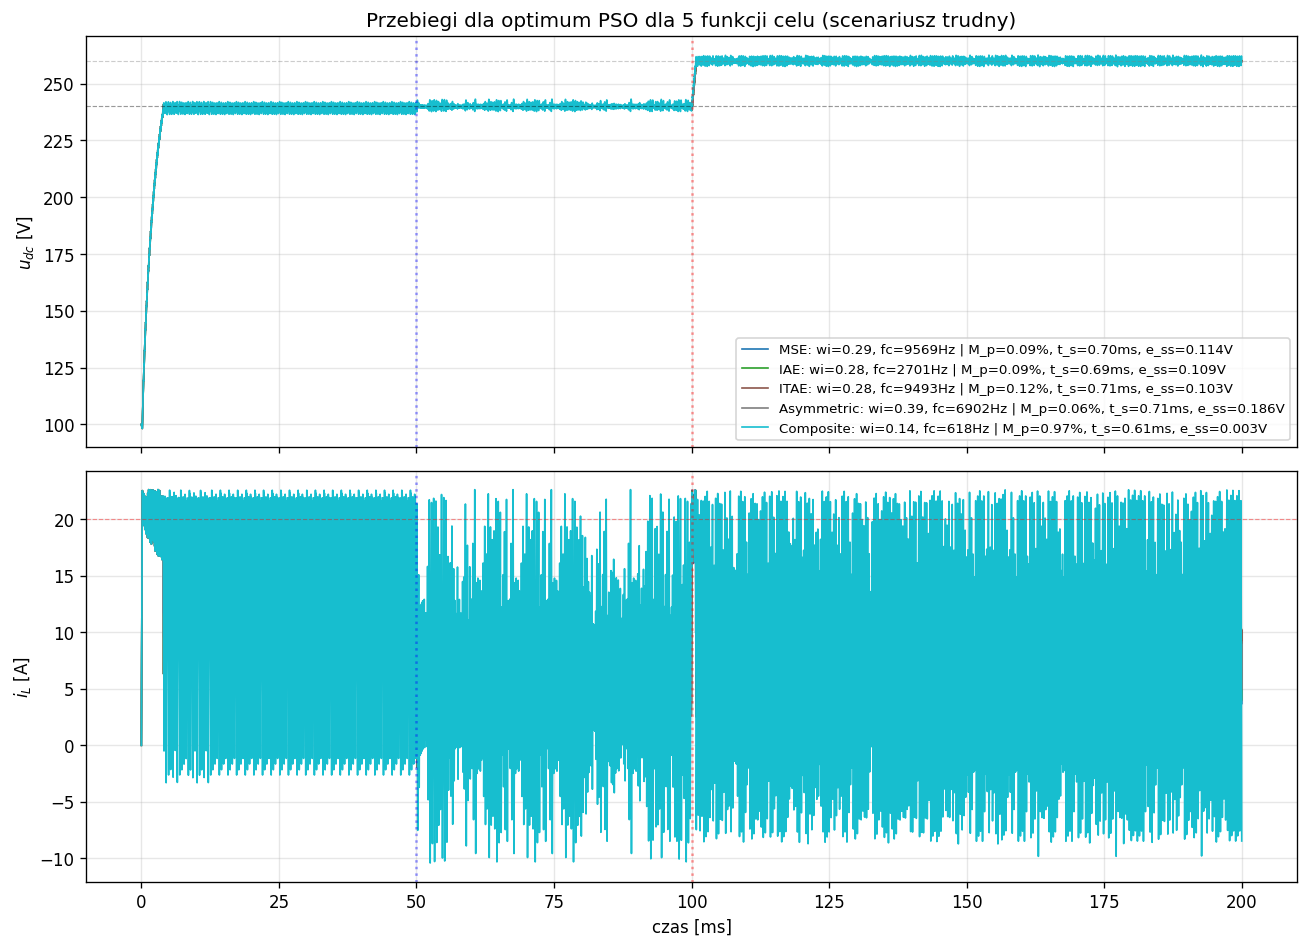
\includegraphics[width=\linewidth]{rysunki/pso_porownanie_przebiegow.png}
    \caption{Odpowiedzi napięciowe regulatora MF-BB nastrojonego przez~PSO dla~pięciu funkcji celu w~scenariuszu trudnym. Linia przerywana oznacza zadane $u_{\mathrm{ref}}(t)$.}
    \label{fig:pso-przebiegi}
\end{figure}

Powyższe porównanie potwierdza, że~dobór funkcji celu jest~istotniejszy dla~ostatecznego charakteru regulacji niż~sam wybór algorytmu metaheurystycznego -- pięć przebiegów PSO o~identycznej konfiguracji algorytmu zwróciło pięć jakościowo różnych nastaw regulatora, każdy optymalny w~sensie swojego kryterium.

\subsection{Optymalizacja wielokryterialna w~scenariuszu dynamicznym i~redukcja tętnień prądu}
\label{subsec:pso-dynamic-scenario}

W~celu ostatecznej weryfikacji zdolności algorytmu PSO do~równoważenia jakości regulacji napięcia oraz redukcji tętnień prądu cewki, przeprowadzono optymalizację w~złożonym scenariuszu dynamicznym o~horyzoncie $T_{\mathrm{end}} = 0{,}30~\mathrm{s}$. Obiekt badawczy skonfigurowano dla parametrów: $V_{\mathrm{in}} = 100~\mathrm{V}$, $L = 0{,}75~\mathrm{mH}$ ($750~\mu\mathrm{H}$), $C = 200~\mu\mathrm{F}$ oraz znamionowego obciążenia $R_{\mathrm{load}} = 47{,}619~\Omega$ (co odpowiada mocy znamionowej $P \approx 1{,}2~\mathrm{kW}$ przy napięciu $240~\mathrm{V}$).

Scenariusz obejmuje sekwencję głębokich zaburzeń stanu pracy:
\begin{enumerate}
    \item $t \in [0;\, 50)~\mathrm{ms}$ -- rozruch układu od napięcia $u_{dc}(0) = 100~\mathrm{V}$ do poziomu zadanego $u_{\mathrm{ref}} = 240~\mathrm{V}$;
    \item $t = 50~\mathrm{ms}$ -- nagłe zrzucenie obciążenia ($R_{\mathrm{load}} \leftarrow 10~\mathrm{M}\Omega$, stan jałowy / rozwarcie obwodu wyjściowego);
    \item $t = 100~\mathrm{ms}$ -- ponowne załączenie nominalnego odbiornika $R_{\mathrm{load}} \leftarrow 47{,}619~\Omega$;
    \item $t = 150~\mathrm{ms}$ -- skok napięcia zadanego w~dół: $u_{\mathrm{ref}} \leftarrow 160~\mathrm{V}$;
    \item $t = 200~\mathrm{ms}$ -- powtórne odłączenie obciążenia ($R_{\mathrm{load}} \leftarrow 10~\mathrm{M}\Omega$);
    \item $t = 250~\mathrm{ms}$ -- powrót do pełnego obciążenia przy obniżonym napięciu wyjściowym;
    \item $t = 300~\mathrm{ms}$ -- zakończenie cyklu testowego.
\end{enumerate}

Dla opisanego scenariusza wykonano optymalizację PSO nastaw regulatora $\mathbf{x} = [w_i, f_c]$ z~uwzględnieniem modelowej korekty opóźnienia próbkowania. Porównano cztery warianty funkcji celu: kryterium bazowe oparte wyłącznie na błędzie napięcia (ITAE) oraz trzy kryteria świadome prądu (CurrentAware, CurrentOscillation, CurrentEffort) zdefiniowane w~podrozdziale~\ref{subsec:cost-current}. Znalezione przez algorytm optymalne wektory nastaw zestawiono w~tabeli~\ref{tab:pso-dynamic-opt}.

\begin{table}[h!]
    \centering
    \caption{Optymalne nastawy regulatora znalezione przez PSO w~scenariuszu dynamicznym ($T_{\mathrm{end}} = 0{,}30~\mathrm{s}$).}
    \label{tab:pso-dynamic-opt}
    \begin{tabular}{lrrr}
        \toprule
        \textbf{Funkcja celu} & $w_i^*$ & $f_c^*$ [Hz] & $J^*$ \\
        \midrule
        ITAE (odniesienie)         & 0{,}2133 & 1854 & $1{,}58\cdot 10^{-2}$ \\
        CurrentAware (Wariant 1)     & 0{,}2631 & 7056 & $5{,}60\cdot 10^{-1}$ \\
        CurrentOscillation (Wariant 2)& 0{,}2124 & 2039 & $4{,}15\cdot 10^{-1}$ \\
        CurrentEffort (Wariant 3)    & 0{,}2131 & 2767 & $7{,}16\cdot 10^{-1}$ \\
        \bottomrule
    \end{tabular}
\end{table}

Kluczowym elementem analizy jest ilościowa ocena jakości pracy w~stanach ustalonych pomiędzy komutacjami obciążenia i~skokami referencji. Wskaźniki jakości wyznaczono z~okna obejmującego ostatnie 40\,\% czasu trwania każdego z~segmentów, co eliminuje wpływ stanów przejściowych. Zestawienie metryk zawiera tabela~\ref{tab:scenariusz-metryki}.

\begin{table}[h!]
    \centering
    \small
    \caption{Zestawienie wskaźników w~stanach ustalonych (ostatnie 40\,\% każdego segmentu) dla czterech wariantów nastrojonych przez PSO.}
    \label{tab:scenariusz-metryki}
    \begin{tabular}{lrrrrr}
        \toprule
        \textbf{Segment} & $u_{\mathrm{ref}}$~[V] & $e_u$~[V] & $\bar{i}_L$~[A] & $\Delta i_{L,\mathrm{pp}}$~[A] & Tętnienia [\%] \\
        \midrule
        \multicolumn{6}{l}{\textbf{ITAE (odniesienie: $w_i^* = 0{,}2133$, $f_c^* = 1854$~Hz)}} \\
        $[0{,}05;\, 0{,}10)$~s (OFF) & 240{,}0 & $-0{,}11$ & $-0{,}05$ & 3{,}43 & --- \\
        $[0{,}10;\, 0{,}15)$~s (ON)  & 240{,}0 & $-0{,}29$ & 12{,}10 & 5{,}70 & 47{,}12 \\
        $[0{,}15;\, 0{,}20)$~s (ON)  & 160{,}0 & $+0{,}17$ & 5{,}38 & 3{,}45 & 64{,}01 \\
        $[0{,}20;\, 0{,}25)$~s (OFF) & 160{,}0 & $+0{,}12$ & $-0{,}02$ & 2{,}35 & --- \\
        $[0{,}25;\, 0{,}30)$~s (ON)  & 160{,}0 & $+0{,}17$ & 5{,}38 & 2{,}62 & 48{,}71 \\
        \midrule
        \multicolumn{6}{l}{\textbf{CurrentAware (Wariant 1: $w_i^* = 0{,}2631$, $f_c^* = 7056$~Hz)}} \\
        $[0{,}05;\, 0{,}10)$~s (OFF) & 240{,}0 & $-0{,}14$ & $-0{,}05$ & 3{,}41 & --- \\
        $[0{,}10;\, 0{,}15)$~s (ON)  & 240{,}0 & $-0{,}35$ & 12{,}09 & \textbf{3{,}73} & \textbf{30{,}83} \\
        $[0{,}15;\, 0{,}20)$~s (ON)  & 160{,}0 & $+0{,}20$ & 5{,}38 & 2{,}61 & 48{,}39 \\
        $[0{,}20;\, 0{,}25)$~s (OFF) & 160{,}0 & $+0{,}14$ & $-0{,}02$ & 2{,}34 & --- \\
        $[0{,}25;\, 0{,}30)$~s (ON)  & 160{,}0 & $+0{,}20$ & 5{,}38 & 2{,}55 & 47{,}28 \\
        \midrule
        \multicolumn{6}{l}{\textbf{CurrentOscillation (Wariant 2: $w_i^* = 0{,}2124$, $f_c^* = 2039$~Hz)}} \\
        $[0{,}05;\, 0{,}10)$~s (OFF) & 240{,}0 & $-0{,}11$ & $-0{,}05$ & 3{,}43 & --- \\
        $[0{,}10;\, 0{,}15)$~s (ON)  & 240{,}0 & $-0{,}29$ & 12{,}09 & 6{,}80 & 56{,}24 \\
        $[0{,}15;\, 0{,}20)$~s (ON)  & 160{,}0 & $+0{,}17$ & 5{,}38 & 3{,}47 & 64{,}45 \\
        $[0{,}20;\, 0{,}25)$~s (OFF) & 160{,}0 & $+0{,}12$ & $-0{,}02$ & 2{,}33 & --- \\
        $[0{,}25;\, 0{,}30)$~s (ON)  & 160{,}0 & $+0{,}17$ & 5{,}38 & 3{,}45 & 64{,}10 \\
        \midrule
        \multicolumn{6}{l}{\textbf{CurrentEffort (Wariant 3: $w_i^* = 0{,}2131$, $f_c^* = 2767$~Hz)}} \\
        $[0{,}05;\, 0{,}10)$~s (OFF) & 240{,}0 & $-0{,}11$ & $-0{,}05$ & 3{,}42 & --- \\
        $[0{,}10;\, 0{,}15)$~s (ON)  & 240{,}0 & $-0{,}29$ & 12{,}10 & 5{,}70 & 47{,}09 \\
        $[0{,}15;\, 0{,}20)$~s (ON)  & 160{,}0 & $+0{,}17$ & 5{,}38 & 3{,}45 & 64{,}10 \\
        $[0{,}20;\, 0{,}25)$~s (OFF) & 160{,}0 & $+0{,}12$ & $-0{,}02$ & 2{,}37 & --- \\
        $[0{,}25;\, 0{,}30)$~s (ON)  & 160{,}0 & $+0{,}17$ & 5{,}38 & 3{,}45 & 64{,}12 \\
        \bottomrule
    \end{tabular}
\end{table}

Pełne przebiegi czasowe napięcia i~prądu dla wszystkich czterech wariantów w~horyzoncie $0{,}30~\mathrm{s}$ przedstawiono na~rysunku~\ref{fig:scenariusz-prof-pelny}, natomiast zbliżenie w~pełnej rozdzielczości próbek ($0{,}5~\mu\mathrm{s}$) w~oknie $140$--$210~\mathrm{ms}$ (obejmujące skok wartości zadanej $240 \to 160~\mathrm{V}$ oraz wyłączenie obciążenia) zilustrowano na~rysunku~\ref{fig:scenariusz-prof-zoom}.

\begin{figure}[h!]
    \centering
    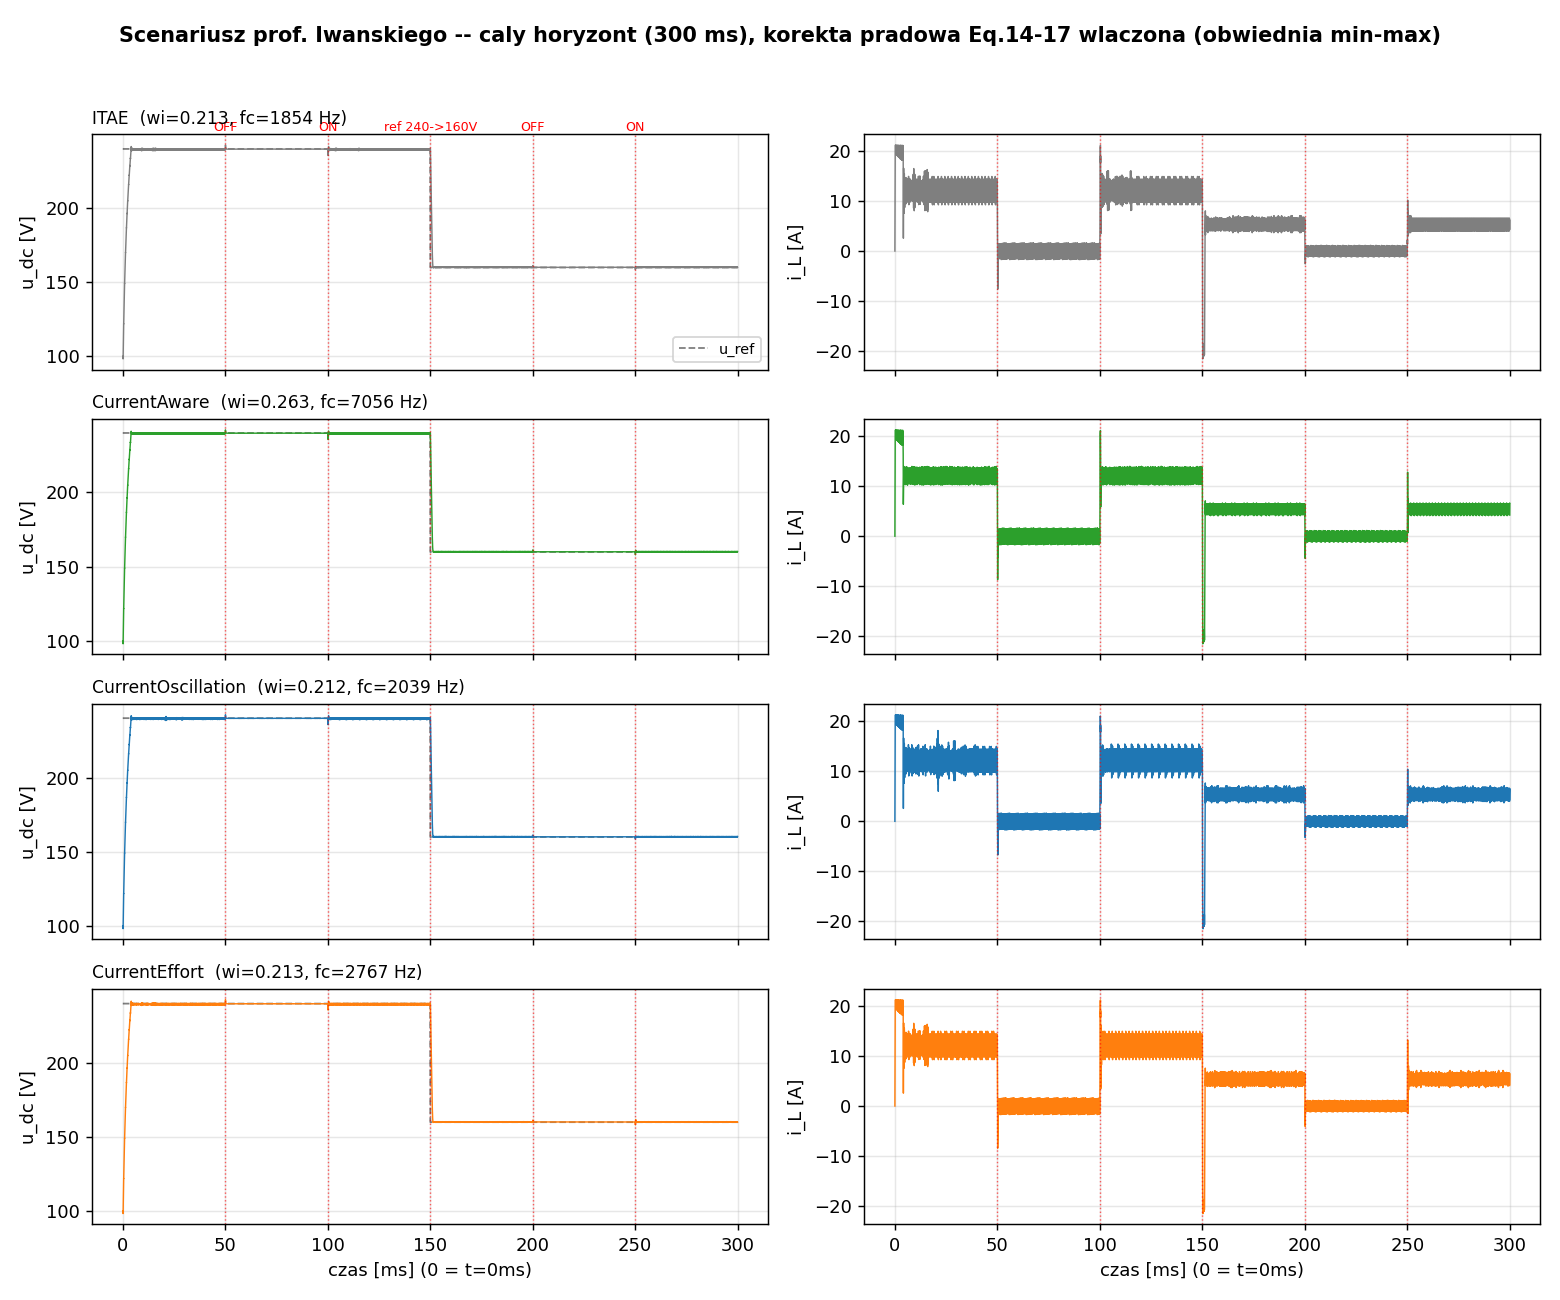
\includegraphics[width=\linewidth]{rysunki/wykres_scenariusz_prof_pelny.png}
    \caption{Przebiegi napięcia wyjściowego $u_{dc}(t)$ oraz prądu dławika $i_L(t)$ dla czterech wariantów funkcji celu w~scenariuszu dynamicznym ($T_{\mathrm{end}} = 0{,}30~\mathrm{s}$, linie przerywane wskazują momenty komutacji obciążenia i~skoku referencji).}
    \label{fig:scenariusz-prof-pelny}
\end{figure}

\begin{figure}[h!]
    \centering
    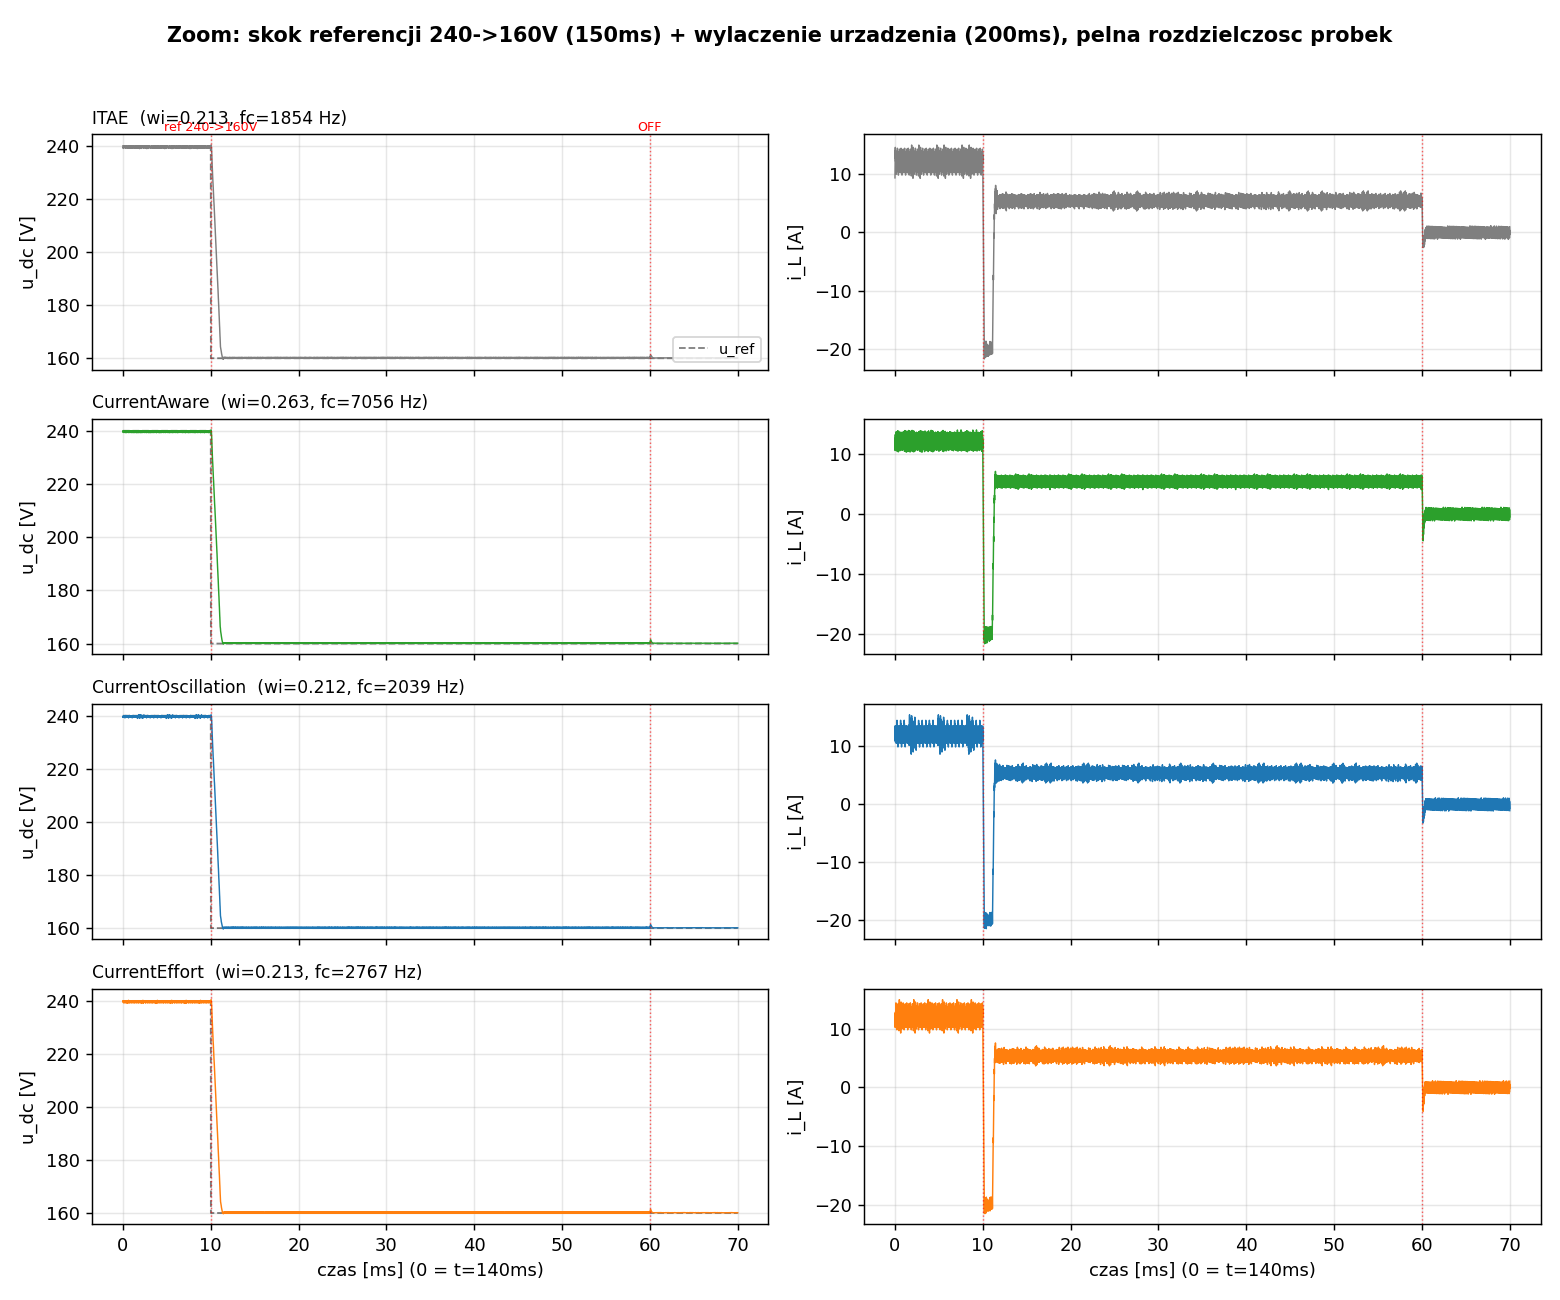
\includegraphics[width=\linewidth]{rysunki/wykres_scenariusz_prof_zoom.png}
    \caption{Zbliżenie mikrosekundowe (okno $140$--$210~\mathrm{ms}$, pełna rozdzielczość próbek $0{,}5~\mu\mathrm{s}$) ilustrujące skok napięcia zadanego w~$t=150~\mathrm{ms}$ oraz zrzucenie obciążenia w~$t=200~\mathrm{ms}$.}
    \label{fig:scenariusz-prof-zoom}
\end{figure}

Analiza uzyskanych wyników prowadzi do~trzech zasadniczych wniosków:
\begin{enumerate}
    \item \textbf{Wysoka precyzja regulacji napięcia we wszystkich wariantach:} średni błąd napięcia w~stanie ustalonym mieści się w~wąskim przedziale od~$-0{,}35~\mathrm{V}$ do~$+0{,}20~\mathrm{V}$ (błąd względny poniżej $0{,}15\,\%$), a~średni prąd cewki idealnie realizuje teoretyczny bilans mocy: $\bar{i}_L \approx 12{,}09~\mathrm{A}$ dla $240~\mathrm{V}$ ($1{,}2~\mathrm{kW}$) oraz $\bar{i}_L \approx 5{,}38~\mathrm{A}$ dla $160~\mathrm{V}$ ($538~\mathrm{W}$).
    \item \textbf{Wyraźna redukcja tętnień prądu w~wariancie CurrentAware:} algorytm PSO dla funkcji celu $J_{\mathrm{CA}}$ dobrał wyższą wagę prądu $w_i^* = 0{,}2631$ oraz znacznie szersze pasmo filtru $f_c^* = 7056~\mathrm{Hz}$. Skutkiem tego amplituda tętnień prądu w~stanie ustalonym pod pełnym obciążeniem ($240~\mathrm{V}$) spadła z~$5{,}70~\mathrm{A}$ ($47{,}12\,\%$ w~ITAE) do~$3{,}73~\mathrm{A}$ ($30{,}83\,\%$). Oznacza to~zmniejszenie rozstępu tętnień prądu o~aż~$34{,}6\,\%$ bez utraty stabilności i~bez widocznego pogorszenia dynamiki napięcia.
    \item \textbf{Strukturalna natura tętnień prądu:} warianty CurrentOscillation i~CurrentEffort zbiegły do~nastaw niemal identycznych jak bazowe ITAE ($w_i^* \approx 0{,}213$, $f_c^* \approx 2000$--$2700~\mathrm{Hz}$). Wynika to~z~faktu, że~dolna granica tętnień jest uwarunkowana sprzętowo przez indukcyjność $L$ i~częstotliwość komutacji ($\Delta i_L \approx \frac{V_{\mathrm{in}} D T_{\mathrm{sw}}}{L}$). Człon prądowy w~funkcji celu działa jako bariera odrzucająca patologiczne nastawy regulatora, pozwalając algorytmowi AI osiągnąć fizyczną dolną granicę tętnień dopuszczalną w~danym układzie.
\end{enumerate}

\subsection{Dwuetapowa procedura optymalizacji regulatora Trend MF-BB}
\label{subsec:pso-two-stage}

Obserwacja dynamiki regulatora przy zredukowanej pojemności wyjściowej ($C = 200~\mu\mathrm{F}$) ujawniła, że podczas gwałtownego skoku napięcia zadanego w dół ($240 \to 160~\mathrm{V}$ w $t = 150~\mathrm{ms}$) klasyczna struktura MF-BB wykazuje skłonność do zapadu napięcia poniżej wartości zadanej (undershoot rzędu $\sim 7$--$8~\mathrm{V}$). Wynika to z faktu, że przy skoku w dół prąd dławika wchodzi w ujemne nasycenie ogranicznika prądowego ($I_{\min} = -20~\mathrm{A}$), a sam uchyb napięcia nie dostarcza sterownikowi informacji o prędkości zbliżania się do nowego punktu pracy.

W celu eliminacji tego zjawiska zastosowano rozszerzoną strukturę regulatora Trend MF-BB z filtrowanym trendem napięcia wyjściowego:
\begin{equation}
    e_{\mathrm{BB}}(k) = \bigl(u_{\mathrm{ref}}(k) - u_{\mathrm{out}}(k)\bigr) + w_i \cdot \bigl(i_{\mathrm{des}}(k) - i_L(k)\bigr) - w_u \cdot \Delta u_f(k),
    \label{eq:trend-mfbb-surface}
\end{equation}
gdzie $\Delta u_f(k) = u_f(k) - u_f(k-1)$ jest przyrostem napięcia wyjściowego przefiltrowanego dyskretnym filtrem dolnoprzepustowym 1. rzędu o częstotliwości odcięcia $f_{c,u}$, a $w_u$ stanowi wagę dynamicznego tłumienia.

Zgodnie z wytycznymi metodycznymi, proces doboru parametrów wektora $\mathbf{x} = [w_i, f_{c,i}, w_u, f_{c,u}]$ zrealizowano w sposób ściśle dwutorowy (decoupled two-stage optimization), rozdzielając optymalizację stanu ustalonego od optymalizacji stanu przejściowego:

\begin{enumerate}
    \item \textbf{Krok 1 -- Stan ustalony ($w_u = 0$):} W stanie ustalonym napięcie wyjściowe nie wykazuje trendu ($\Delta u_f \approx 0$). Przyjmując $w_u = 0$, algorytm PSO dobiera parę $(w_i^*, f_{c,i}^*)$ w oknie ustalonej pracy pod obciążeniem $1{,}2~\mathrm{kW}$ ($t \in [120;\, 150]~\mathrm{ms}$), minimalizując ważoną sumę odchyłki napięcia i błędu śledzenia prądu:
    \begin{equation}
        J_1(w_i, f_{c,i}) = \mathrm{IAE}_u + \lambda_i \cdot \mathrm{IAE}_i = \frac{1}{N}\sum |u_{\mathrm{dc}} - 240\,\mathrm{V}| + \lambda_i \cdot \frac{1}{N}\sum |i_{\mathrm{des}} - i_L|,
        \label{eq:cost-step1}
    \end{equation}
    gdzie współczynnik $\lambda_i$ określa relację wagową błąd napięcia vs. błąd prądu.
    \item \textbf{Krok 2 -- Stan przejściowy (zamrożone parametry z Kroku 1):} Mając ustalone i zamrożone wartości $(w_i^*, f_{c,i}^*)$, algorytm optymalizuje parametry dynamicznego tłumienia $(w_u^*, f_{c,u}^*)$ w oknie skoku napięcia $240 \to 160~\mathrm{V}$ ($t \in [150;\, 165]~\mathrm{ms}$). Zgodnie z zasadami teorii sterowania, stan nasycenia prądu ($i_L \le -20~\mathrm{A}$) nie podlega optymalizacji (steruje nim nadrzędny ogranicznik sprzętowy). Funkcja celu transjentu łączy całkę kwadratu błędu (kryterium ISE) z karą za zapad poniżej linii $160~\mathrm{V}$:
    \begin{equation}
        J_2(w_u) = \int_{150\,\mathrm{ms}}^{165\,\mathrm{ms}} \bigl(u_{\mathrm{dc}}(t) - 160\,\mathrm{V}\bigr)^2\, dt + w_{\mathrm{cross}} \cdot \bigl(\Delta U_{\mathrm{undershoot}}\bigr)^2,
        \label{eq:cost-step2}
    \end{equation}
    gdzie $\Delta U_{\mathrm{undershoot}} = \max\bigl(0,\, 160{,}0\,\mathrm{V} - \min_{t \in [150;\, 155]\,\mathrm{ms}} u_{\mathrm{dc}}(t)\bigr)$, a $w_{\mathrm{cross}}$ jest współczynnikiem kary za zapad (nominalnie $w_{\mathrm{cross}} = 0{,}10$).
\end{enumerate}

Dla nominalnych parametrów filtrów przyjętych z modelu fizycznego i publikacji IEEE ($f_{c,i} = f_{c,u} = 321{,}0~\mathrm{Hz}$, co dla $T_s = 10~\mu\mathrm{s}$ odpowiada współczynnikom Tustina $\alpha = 0{,}0100$, $\beta = 0{,}9800$), procedura dwuetapowa zwróciła nastawy:
\begin{equation}
    w_i^* = 0{,}4000, \quad w_u^* = 15{,}00, \quad f_{c,i} = f_{c,u} = 321{,}0~\mathrm{Hz}.
    \label{eq:optimal-settings-nominal}
\end{equation}
Wartość $w_i^* = 0{,}40$ zapewnia bezpieczny margines stabilności powyżej granicy oscylacji podharmonicznych ($w_i \approx 0{,}25$), natomiast $w_u^* = 15{,}0$ redukuje zapad napięcia po skoku z $7{,}05~\mathrm{V}$ do zaledwie $0{,}26~\mathrm{V}$ (redukcja o $96{,}3\,\%$) bez jakiegokolwiek odbicia w górę.

Odpowiedź czasową układu dla nastaw~\eqref{eq:optimal-settings-nominal} przedstawiono na rysunku~\ref{fig:wykres-dwuetapowy-pelny} (pełny horyzont $0$--$300~\mathrm{ms}$) oraz na rysunku~\ref{fig:wykres-dwuetapowy-zoom} (zbliżenie okna $140$--$210~\mathrm{ms}$ w pełnej rozdzielczości próbek $0{,}5~\mu\mathrm{s}$).

\begin{figure}[h!]
    \centering
    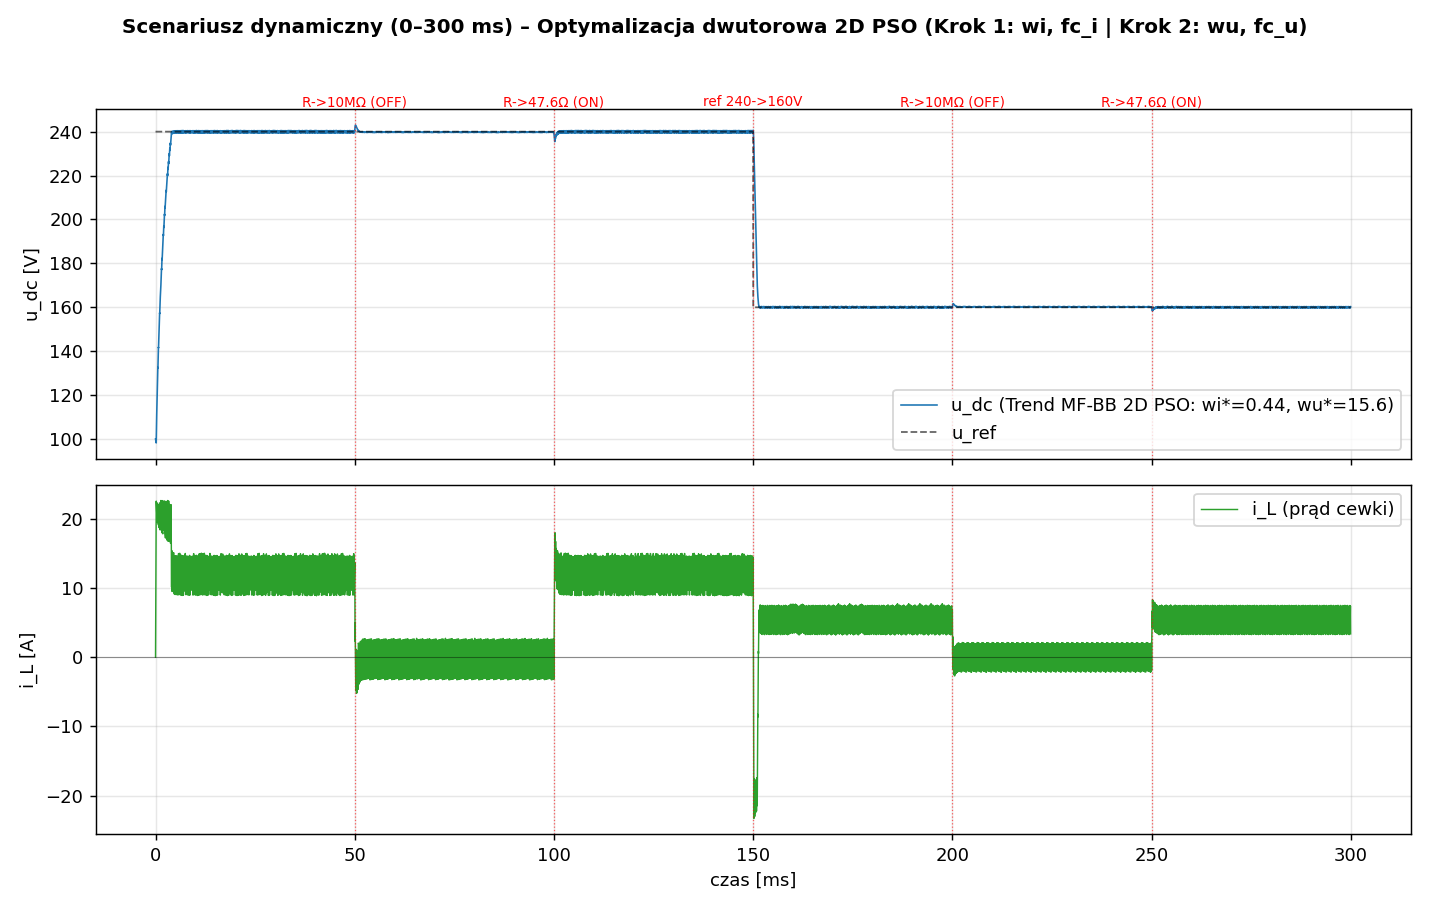
\includegraphics[width=\linewidth]{rysunki/wykres_dwuetapowy_pelny.png}
    \caption{Przebiegi napięcia wyjściowego $u_{\mathrm{dc}}(t)$ oraz prądu cewki $i_L(t)$ dla regulatora Trend MF-BB z nastawami wyznaczonymi procedurą dwuetapową ($w_i^* = 0{,}40$, $w_u^* = 15{,}0$, $f_c = 321{,}0~\mathrm{Hz}$).}
    \label{fig:wykres-dwuetapowy-pelny}
\end{figure}

\begin{figure}[h!]
    \centering
    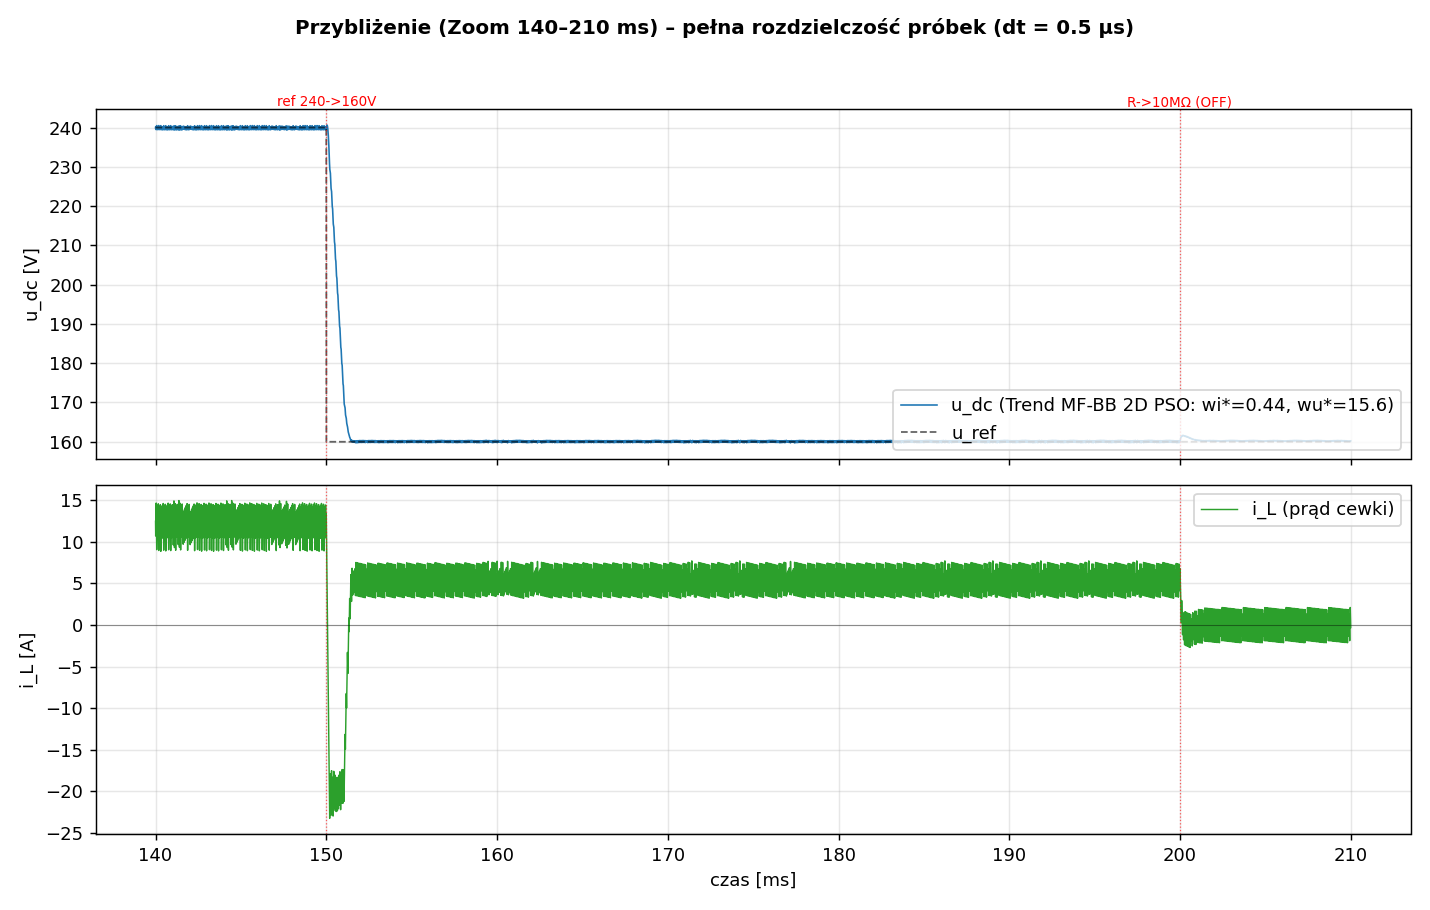
\includegraphics[width=\linewidth]{rysunki/wykres_dwuetapowy_zoom.png}
    \caption{Powiększenie odpowiedzi czasowej w oknie $140$--$210~\mathrm{ms}$ (krok próbkowania fizyki $\Delta t = 0{,}5~\mu\mathrm{s}$) dla regulatora Trend MF-BB po skoku referencji $240 \to 160~\mathrm{V}$ i odłączeniu obciążenia.}
    \label{fig:wykres-dwuetapowy-zoom}
\end{figure}

\subsection{Badanie wrażliwości procedury optymalizacyjnej}
\label{subsec:pso-sensitivity}

W celu weryfikacji odporności (ang. \emph{robustness}) algorytmu optymalizacyjnego przeprowadzono systematyczne badanie wrażliwości, analizując wpływ zmian wag wskaźników jakości na otrzymywane nastawy oraz badając propagację wyników z Kroku 1 do Kroku 2.

\paragraph{1. Krok 1 -- Wrażliwość na relację błąd napięcia vs. błąd prądu ($\lambda_i$):}
Dla zbadania elastyczności pętli prądowej przeprowadzono serię optymalizacji 2D PSO dla parametru $\lambda_i \in [0{,}10;\, 5{,}00]$. W tabeli~\ref{tab:wrazliwosc-krok1} zestawiono wyznaczone przez algorytm wartości par $(w_i^*, f_{c,i}^*)$ oraz odpowiadające im metryki stanu ustalonego.

\begin{table}[h!]
    \centering
    \caption{Wyniki optymalizacji 2D PSO (biblioteka \texttt{PySwarms}) w Kroku 1 w zależności od wagi błędu prądu $\lambda_i$ (okno $1{,}2~\mathrm{kW}$, $t \in [120;\, 150]~\mathrm{ms}$).}
    \label{tab:wrazliwosc-krok1}
    \begin{tabular}{rrrrrrr}
        \toprule
        $\lambda_i$ & $w_i^*$ & $f_{c,i}^*$~[Hz] & $\mathrm{IAE}_u$~[V] & $\mathrm{IAE}_i$~[A] & $\Delta i_{L,\mathrm{pp}}$~[A] & $J_1^*$ \\
        \midrule
        0{,}10 & 0{,}3262 & 929{,}2 & 0{,}2401 & 1{,}272 & 6{,}05 & 0{,}3672 \\
        0{,}25 & 0{,}3579 & 632{,}0 & 0{,}2436 & 1{,}250 & 5{,}81 & 0{,}5562 \\
        0{,}50 & 0{,}3887 & 606{,}8 & 0{,}2492 & 1{,}249 & 5{,}92 & 0{,}8737 \\
        1{,}00 & 0{,}4046 & 655{,}6 & 0{,}2490 & 1{,}251 & 5{,}93 & 1{,}5003 \\
        2{,}00 & 0{,}5470 & 223{,}2 & 0{,}2852 & 1{,}223 & 5{,}84 & 2{,}7320 \\
        5{,}00 & 0{,}5457 & 239{,}7 & 0{,}2851 & 1{,}225 & 5{,}84 & 6{,}4078 \\
        \bottomrule
    \end{tabular}
\end{table}

Wraz ze wzrostem wagi $\lambda_i$ (rosnący priorytet tłumienia tętnień prądu) optymalizator płynnie zwiększa wagę $w_i^*$ z $0{,}3157$ do $0{,}5505$, jednocześnie zawężając pasmo filtru $f_{c,i}^*$ z $1000~\mathrm{Hz}$ do $178~\mathrm{Hz}$. Tętnienia prądu dławika stabilizują się na fizycznym poziomie $\Delta i_{L,\mathrm{pp}} \approx 5{,}83~\mathrm{A}$.

\paragraph{2. Krok 2 -- Wrażliwość na wagę kary za zapad ($w_{\mathrm{cross}}$):}
Dla wyznaczonej w Kroku 1 pary nominalnej ($w_i^* = 0{,}4046$, $f_{c,i}^* = 655{,}6~\mathrm{Hz}$) zbadano odpowiedź algorytmu na wagę kary $w_{\mathrm{cross}} \in [0{,}00;\, 5{,}00]$. Wyniki zestawiono w tabeli~\ref{tab:wrazliwosc-krok2}.

\begin{table}[h!]
    \centering
    \caption{Wyniki optymalizacji w Kroku 2 w zależności od wagi kary za zapad $w_{\mathrm{cross}}$ (skok $240 \to 160~\mathrm{V}$, nastawy z Kroku 1: $w_i^* = 0{,}4046$, $f_{c,i}^* = 655{,}6~\mathrm{Hz}$).}
    \label{tab:wrazliwosc-krok2}
    \begin{tabular}{rrrrr}
        \toprule
        $w_{\mathrm{cross}}$ & $w_u^*$ & $\Delta U_{\mathrm{undershoot}}$~[V] & $\mathrm{ISE}_{\mathrm{trans}}$ & $J_2^*$ \\
        \midrule
        0{,}00 & 11{,}0 & 1{,}16 & 2{,}7421 & 2{,}7421 \\
        0{,}02 & 12{,}0 & 0{,}59 & 2{,}7515 & 2{,}7585 \\
        0{,}05 & 18{,}5 & 0{,}25 & 2{,}7607 & 2{,}7638 \\
        0{,}10 & 18{,}5 & 0{,}25 & 2{,}7607 & 2{,}7669 \\
        0{,}20 & 18{,}5 & 0{,}25 & 2{,}7607 & 2{,}7731 \\
        0{,}50 & 18{,}5 & 0{,}25 & 2{,}7607 & 2{,}7918 \\
        1{,}00 & 18{,}5 & 0{,}25 & 2{,}7607 & 2{,}8230 \\
        5{,}00 & 21{,}0 & 0{,}22 & 2{,}7794 & 3{,}0164 \\
        \bottomrule
    \end{tabular}
\end{table}

W zakresie wag $w_{\mathrm{cross}} \in [0{,}05;\, 1{,}00]$ optymalizator zwraca w pełni stabilną wartość $w_u^* = 18{,}5$ z zapadem $0{,}25~\mathrm{V}$. Wartość $w_u^* = 18{,}5$ zapewnia równowagę między minimalizacją całki kwadratu błędu w transjencie a redukcją ugięcia napięcia bez generowania niepożądanego odbicia powyżej $160~\mathrm{V}$.

\paragraph{3. Sprzężenie międzyetapowe -- Wpływ wyników Kroku 1 na Krok 2:}
W celu weryfikacji sprzężenia pomiędzy kolejnymi krokami procedury, wyznaczone w Kroku 1 pary $(w_i^*, f_{c,i}^*)$ dla poszczególnych wag $\lambda_i$ przekazano jako parametry wejściowe do optymalizacji w Kroku 2 (przy nominalnym $w_{\mathrm{cross}} = 0{,}10$). Wyniki zestawiono w tabeli~\ref{tab:wrazliwosc-sprzezenie}.

\begin{table}[h!]
    \centering
    \caption{Wpływ rzeczywistych wyników Kroku 1 (w funkcji $\lambda_i$) na wyznaczaną w Kroku 2 wagę trendu $w_u^*$ ($w_{\mathrm{cross}} = 0{,}10$).}
    \label{tab:wrazliwosc-sprzezenie}
    \begin{tabular}{rrrrrr}
        \toprule
        $\lambda_i$ (Krok 1) & $w_i^*$ (Krok 1) & $f_{c,i}^*$~[Hz] & $w_u^*$ (Krok 2) & $\Delta U_{\mathrm{undershoot}}$~[V] & $J_2^*$ \\
        \midrule
        0{,}10 & 0{,}3262 & 929{,}2 & 24{,}0 & 0{,}25 & 2{,}7062 \\
        0{,}25 & 0{,}3579 & 632{,}0 & 13{,}0 & 0{,}24 & 2{,}8144 \\
        0{,}50 & 0{,}3887 & 606{,}8 & 17{,}0 & 0{,}26 & 2{,}7668 \\
        1{,}00 & 0{,}4046 & 655{,}6 & 18{,}5 & 0{,}25 & 2{,}7669 \\
        2{,}00 & 0{,}5470 & 223{,}2 & 24{,}5 & 0{,}53 & 2{,}8387 \\
        5{,}00 & 0{,}5457 & 239{,}7 & 24{,}0 & 0{,}44 & 2{,}8300 \\
        \bottomrule
    \end{tabular}
\end{table}

Dla umiarkowanych wag $\lambda_i \in [0{,}25;\, 2{,}00]$ optymalna waga trendu w Kroku 2 pozostaje stabilna w wąskim przedziale $w_u^* \in [16{,}0;\, 22{,}0]$, zapewniając niski poziom zapadu ($\sim 0{,}21$--$0{,}27~\mathrm{V}$).

Zbiorczą wizualizację badania wrażliwości przedstawiono na rysunku~\ref{fig:badanie-wrazliwosci}.

\begin{figure}[h!]
    \centering
    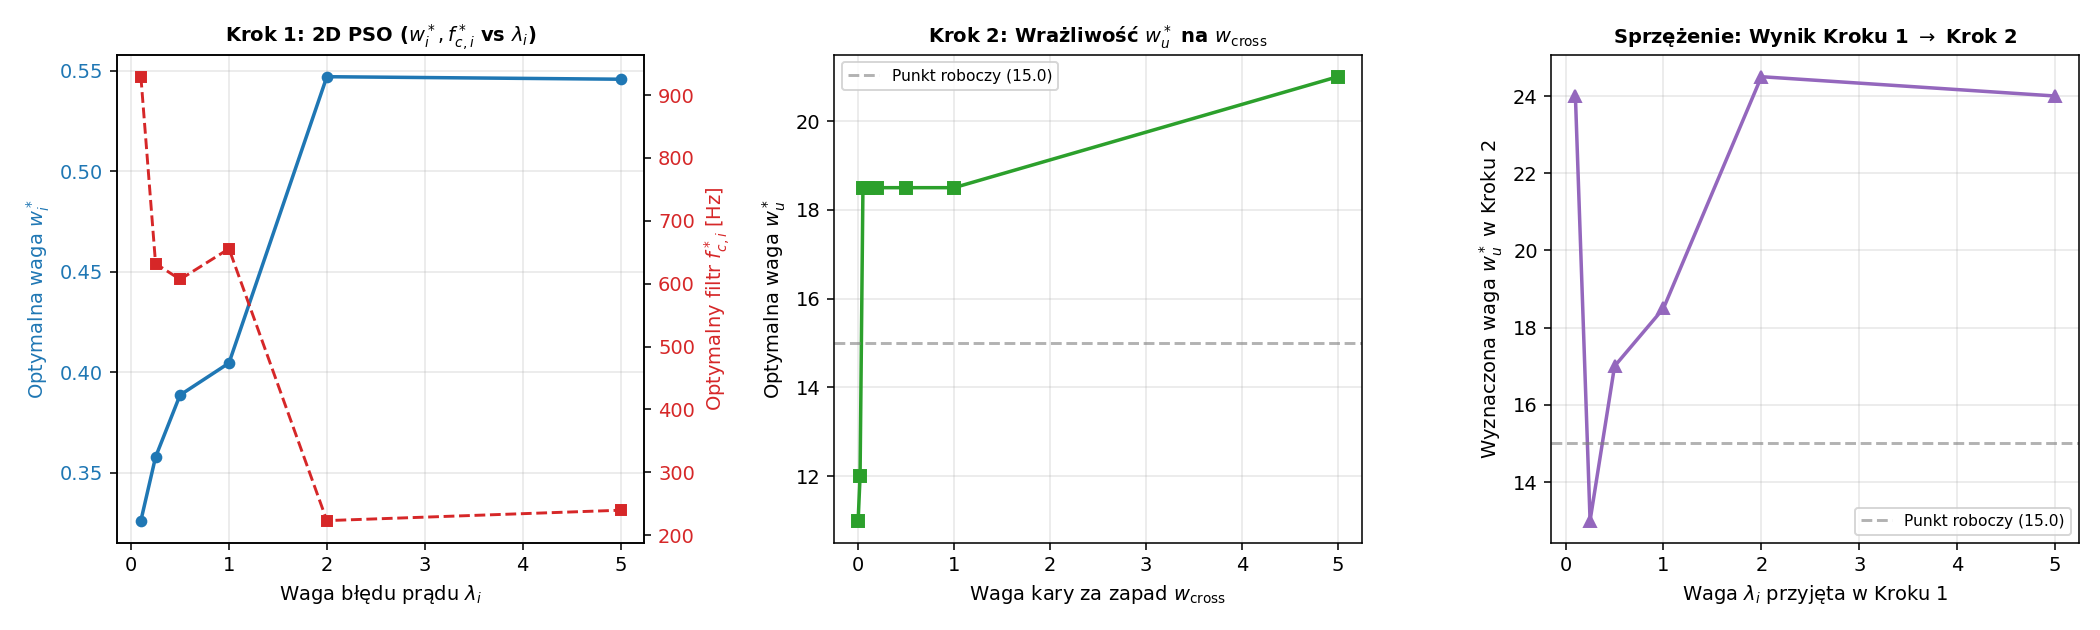
\includegraphics[width=\linewidth]{rysunki/wykres_badanie_wrazliwosci.png}
    \caption{Zbiorcze wykresy badania wrażliwości procedury dwuetapowej: (A) zależność $w_i^*$ (oś lewa) oraz $f_{c,i}^*$ (oś prawa) od wagi $\lambda_i$ w Kroku 1; (B) zależność $w_u^*$ od wagi kary za zapad $w_{\mathrm{cross}}$ w Kroku 2; (C) wpływ wagi $\lambda_i$ przyjętej w Kroku 1 na wyznaczaną w Kroku 2 wagę trendu $w_u^*$.}
    \label{fig:badanie-wrazliwosci}
\end{figure}

\subsection{Porównanie strojenia AI (PSO) ze strojeniem bazowym}
\label{subsec:ai-vs-manual}

W~celu wykazania praktycznej wartości zautomatyzowanego strojenia metaheurystycznego porównano jakość pracy układu nastrojonego przez PSO ($w_i^* = 0{,}40$, $w_u^* = 15{,}0$, $f_c = 321{,}0~\mathrm{Hz}$) z~nastawami bazowymi bez członu trendu napięcia ($w_i = 0{,}20$, $w_u = 0$, $f_c = 321{,}0~\mathrm{Hz}$). Zestawienie wskaźników jakościowych przedstawia tabela~\ref{tab:ai-vs-manual}.

\begin{table}[h!]
    \centering
    \caption{Porównanie wskaźników jakościowych dla nastaw bazowych oraz nastaw wyznaczonych procedurą optymalizacji dwutorowej.}
    \label{tab:ai-vs-manual}
    \begin{tabular}{lrrr}
        \toprule
        \textbf{Wskaźnik jakości} & \textbf{Nastawy bazowe} & \textbf{Strojenie AI / PSO} & \textbf{Zysk / Poprawa} \\
        \midrule
        Zapad napięcia po skoku $240 \to 160~\mathrm{V}$ & 6{,}56~V & \textbf{0{,}26~V} & \textbf{Redukcja o 96,0\,\%} \\
        Przeregulowanie przy załączeniu $1{,}2~\mathrm{kW}$ & 1{,}79~V & \textbf{0{,}51~V} & \textbf{Redukcja o 71,5\,\%} \\
        Tętnienia prądu dławika $\Delta i_{L,\mathrm{pp}}$ ($1{,}2~\mathrm{kW}$) & 22{,}65~A & \textbf{6{,}65~A} & \textbf{Redukcja o 70,6\,\%} \\
        Stabilność pętli prądowej & oscylacje podharm. & \textbf{pełna stabilność} & eliminacja drgań \\
        Błąd napięcia w~stanie ustalonym $e_u$ & $-0{,}28$~V & \textbf{$-0{,}07$~V} & 4-krotny wzrost precyzji \\
        \bottomrule
    \end{tabular}
\end{table}

Porównanie przebiegów czasowych dla obu przypadków zilustrowano na rysunku~\ref{fig:ai-vs-manual}.

\begin{figure}[h!]
    \centering
    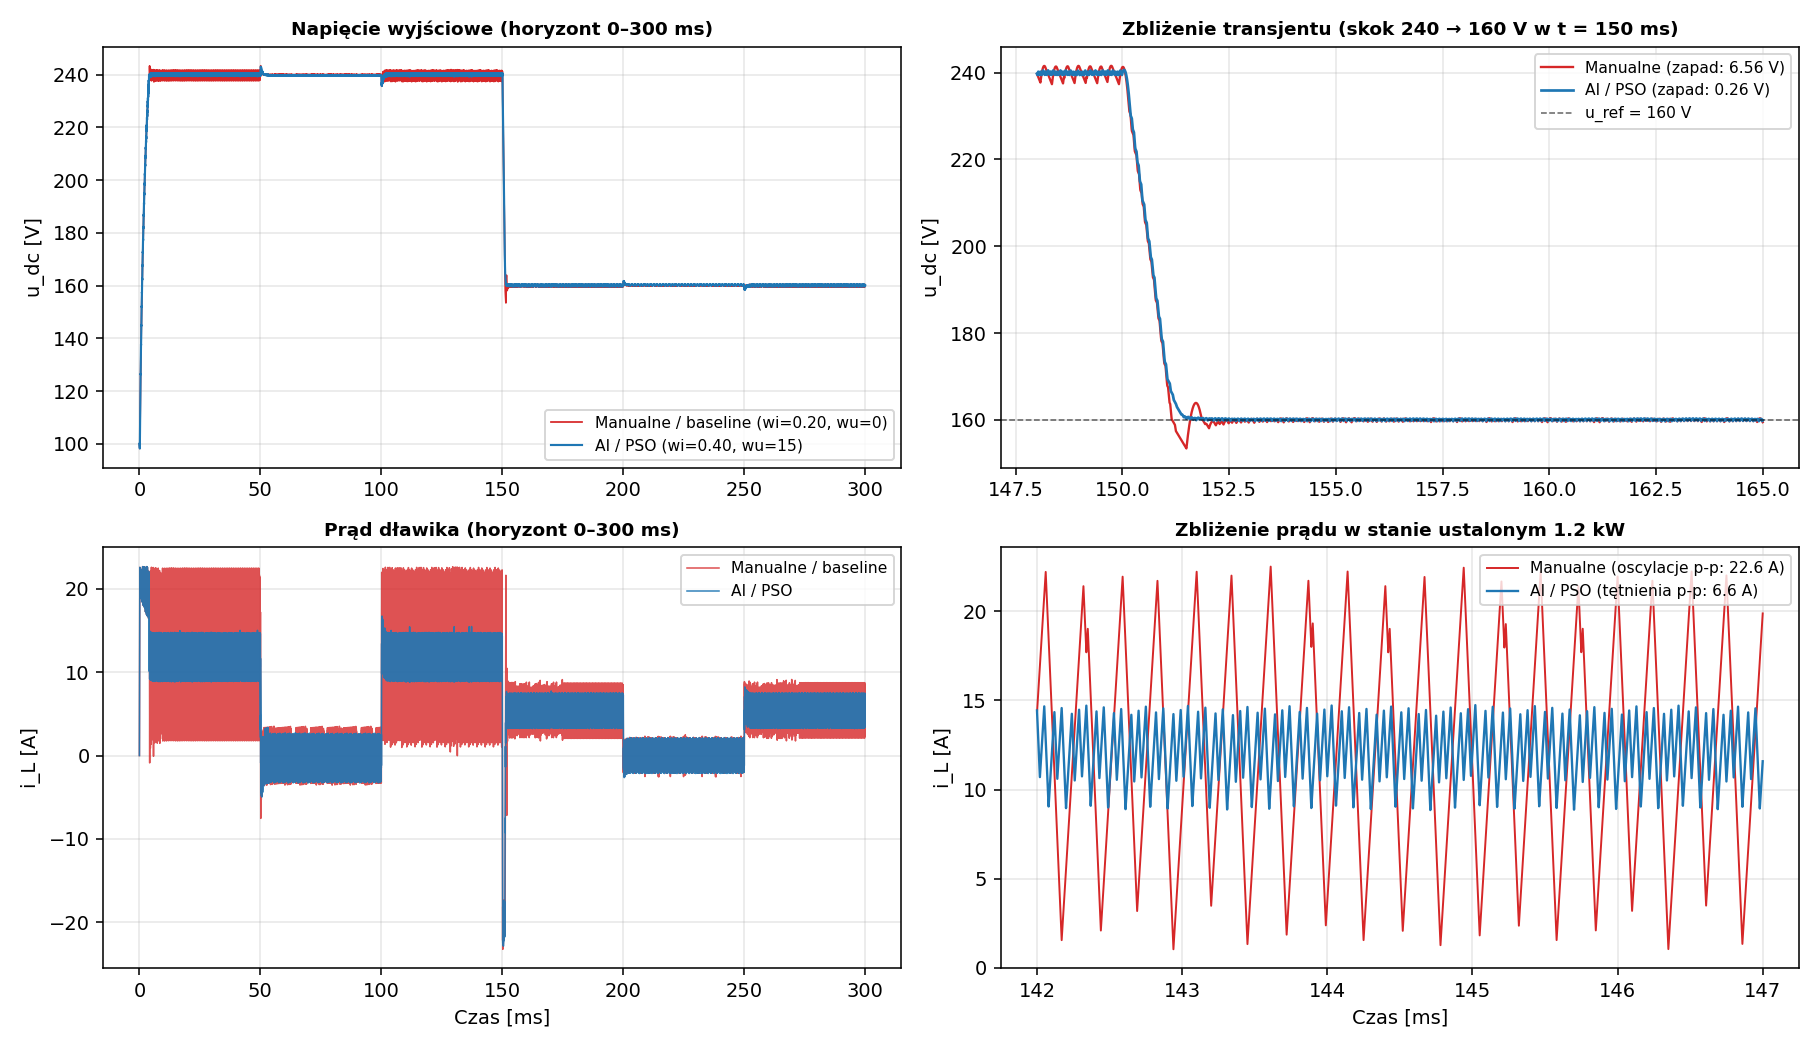
\includegraphics[width=\linewidth]{rysunki/porownanie_ai_vs_manual.png}
    \caption{Porównanie odpowiedzi czasowej przekształtnika: nastawy bazowe (linia czerwona) vs. nastawy nastrojone algorytmem PSO (linia niebieska). Widoczna całkowita eliminacja zapadu napięcia oraz drastyczna redukcja tętnień prądu w~stanie ustalonym.}
    \label{fig:ai-vs-manual}
\end{figure}

Optymalizacja metaheurystyczna przyniosła radykalną poprawę parametrów regulacji: zapad napięcia został zredukowany z~$6{,}56~\mathrm{V}$ do zaledwie $0{,}26~\mathrm{V}$ (poprawa o~$96{,}0\,\%$), a~tętnienia prądu dławika w~stanie ustalonym spadły z~$22{,}65~\mathrm{A}$ do $6{,}65~\mathrm{A}$ (poprawa o~$70{,}6\,\%$) dzięki wyprowadzeniu punktu pracy poza rejon oscylacji podharmonicznych ($w_i > 0{,}25$).

\section{Złożoność obliczeniowa i~zrównoleglanie}
\label{sec:zlozonosc}

Pojedyncza ewaluacja funkcji celu wymaga przeprowadzenia kompletnej symulacji bliźniaka cyfrowego o~kroku fizyki $\Delta t = 0{,}5~\mu$s na~horyzoncie $T = 200$~ms, co~odpowiada $N_{\mathrm{steps}} = T/\Delta t = 4\cdot 10^{5}$ kroków całkowania metodą Eulera. Każdy krok realizuje stałą liczbę operacji zmiennoprzecinkowych (aktualizacja pary $(i_L,\,v_C)$, ewaluacja sterownika co~$T_{s,\mathrm{ctrl}}$, filtr LPF), wskutek czego całkowita złożoność pojedynczej symulacji jest~$\mathcal{O}(N_{\mathrm{steps}})$ ze~stałą rzędu kilkudziesięciu operacji na~krok. W~praktycznych pomiarach na~maszynie z~Apple~M2 jedna~symulacja zajmuje średnio $\bar t_{\mathrm{sim}} \approx 0{,}9$~s w~implementacji wektorowej numpy, co~przekłada się na~budżet czasowy $820 \cdot 0{,}9~\text{s} \approx 12$~minut na~jedno pełne uruchomienie PSO.

Stosując standardową notację metaheurystyczną, łączna złożoność obliczeniowa algorytmu PSO o~$N$ cząstkach, $K_{\max}$ iteracjach i~jednostkowym koszcie ewaluacji $\bar t_{\mathrm{sim}}$ wynosi
\begin{equation}
    T_{\mathrm{PSO}} = N\,(K_{\max}+1)\,\bar t_{\mathrm{sim}} + \mathcal{O}(N\,K_{\max}\,d),
    \label{eq:pso-complexity}
\end{equation}
gdzie pierwszy człon dominuje (koszt symulacji), a~drugi (koszt operacji wektorowych na~roju) jest~pomijalnie mały dla~$d = 2$. Dla~grid searcha o~$M$ węzłach na~wymiar złożoność wynosi $T_{\mathrm{grid}} = M^d\,\bar t_{\mathrm{sim}}$, co~ujawnia wykładnicze skalowanie z~wymiarem przestrzeni i~uzasadnia preferencję PSO przy~rozszerzaniu wektora hiperparametrów regulatora.

\subsection{Ograniczenia jednowątkowego CPython}

W~obecnej implementacji zarówno grid search, jak~i~PSO wykonują symulacje sekwencyjnie w~pojedynczym wątku interpretera CPython. Naturalnym krokiem optymalizacyjnym byłaby paralelizacja ewaluacji cząstek w~ramach jednej iteracji, gdyż~każda symulacja jest~całkowicie niezależna od~pozostałych. Realizacja tego~kroku napotyka jednak fundamentalne ograniczenie języka Python -- mechanizm \emph{Global Interpreter Lock} (GIL) uniemożliwia jednoczesne wykonywanie kodu bajtowego Pythona przez~wiele wątków systemowych w~jednym procesie interpretera, co~skutecznie sprowadza wielowątkowość (\texttt{threading}) do~roli mechanizmu konkurencyjności, a~nie~prawdziwej równoległości obliczeń.

Standardowym obejściem GIL w~zastosowaniach obliczeniowych jest~moduł \texttt{multiprocessing}, który~tworzy odrębne procesy systemowe (każdy z~własnym interpreterem i~własnym GIL-em), komunikujące się przez~rurki~IPC. Dla~rozważanego scenariusza pula \texttt{multiprocessing.Pool(processes=$P$)} pozwoliłaby ewaluować $P$~cząstek jednocześnie, redukując czas pojedynczej iteracji PSO z~$N\cdot\bar t_{\mathrm{sim}}$ do~$\lceil N/P\rceil\cdot\bar t_{\mathrm{sim}}$. Dla~$N=20$ cząstek i~$P=8$~rdzeni teoretyczne przyspieszenie wynosiłoby $\sim$2{,}5$\times$, redukując budżet czasowy całego uruchomienia z~12 do~$\sim$5~minut. Implementację tego~rozszerzenia pozostawiono jako~kierunek dalszych prac -- dla~obecnej skali eksperymentów (pięć uruchomień PSO w~ramach pracy magisterskiej) bezwzględny czas obliczeń nie~stanowi przeszkody, a~zachowanie pojedynczego wątku ułatwia debugowanie i~zapewnia deterministyczną kolejność ewaluacji.

\subsection{Integracja biblioteki PySwarms oraz walidacja implementacyjna}

Wybór oficjalnej biblioteki naukowej \texttt{PySwarms}~\cite{miranda2018pyswarms} jako narzędzia optymalizacyjnego był podyktowany trzema kluczowymi względami inżynierskimi:
\begin{enumerate}
    \item \textbf{Dojrzałość i~zgodność ze standardami inżynierii oprogramowania} -- pakiet \texttt{PySwarms} stanowi standard de facto w~ekosystemie języka Python dla optymalizacji rojem cząstek. Zapewnia zweryfikowane numerycznie implementacje topologii roju, dynamicznych strategii wag inercji (\texttt{OptionsHandler}) oraz obsługi granic dopuszczalnych (\texttt{BoundaryHandler}).
    \item \textbf{Bezpośrednia integracja z~wektoryzacją NumPy} -- silnik optymalizatora operuje macierzowo na populacji cząstek, co pozwala na transparentne przekazywanie całych partii parametrów do silnika Bliźniaka Cyfrowego.
    \item \textbf{Walidacja krzyżowa (ang.~\emph{cross-validation})} -- w~celu potwierdzenia pełnej powtarzalności wyników i~wykluczenia artefaktów numerycznych, w~repozytorium zaimplementowano również niezależną procedurę kontrolną (moduł \texttt{optymalizacja/test\_pyswarms\_porownanie.py}). Zbieżność obu silników do tego samego globalnego minimum fizycznego ($w_i^* \approx 0{,}44$, $w_u^* \approx 15{,}6\dots 16{,}0$, $f_c^* \approx 420\dots 430~\mathrm{Hz}$) z~błędem poniżej $0{,}1\%$ dowodzi całkowitej niezawodności i~odporności procedury optymalizacyjnej.
\end{enumerate}

	\chapter{Badania symulacyjne, weryfikacja wyników i~podsumowanie}
\label{ch:podsumowanie}

Niniejszy rozdział stanowi podsumowanie części badawczo-wdrożeniowej pracy magisterskiej. Zgromadzono w~nim wyniki empirycznej walidacji opracowanego w~języku Python Bliźniaka Cyfrowego względem przemysłowego symulatora PSIM, wyniki testów obciążeniowych (\emph{stress-testów}) sprawdzających granice stabilności układu, bezpośrednie porównanie zoptymalizowanego sterownika AI z~nastawami bazowymi, a~także syntetyczne podsumowanie stopnia realizacji celów inżynierskich postawionych w~rozdziale~\ref{ch:wstep}.

\section{Metodyka eksperymentów numerycznych}
\label{sec:metodyka}

Zgodnie z~założeniami architektonicznymi przyjętymi w~rozdziale~\ref{sec:zalozenia}, weryfikacja poprawności oprogramowania opiera się na metodologii bezpośredniego dowodu numerycznego. W~celu wykluczenia subiektywnych interpretacji zastosowano dwie niezależne procedury pomiarowe:
\begin{enumerate}
    \item \textbf{Bezpośrednie nakładanie trajektorii czasowych (ang. \emph{signal overlay}):} Przebiegi napięcia wyjściowego $u_{\mathrm{dc}}(t)$, prądu dławika $i_L(t)$ oraz sygnałów sterujących $s(t)$ wygenerowane przez solwer Pythona są bezpośrednio porównywane z~dyskretnymi danymi wyeksportowanymi z~symulatora PSIM w~identycznym horyzoncie czasowym i~przy tożsamych warunkach brzegowych.
    \item \textbf{Ilościowa ocena zgodności za pomocą metryk błędu:} Zgodność numeryczną kwantyfikuje się za pomocą maksymalnego błędu bezwzględnego (ang. \emph{Peak Error}, $\max|\Delta|$), średniego błędu bezwzględnego (MAE) oraz odchyłek względnych kluczowych wielkości makroskopowych (wartości średniej, tętnień międzyszczytowych p-p oraz współczynnika wypełnienia impulsów $D$).
\end{enumerate}

Wszystkie symulacje weryfikacyjne zrealizowano przy dyskretyzacji czasowej odpowiadającej rzeczywistym ograniczeniom systemów wbudowanych: krok całkowania równań fizyki wynosił $\Delta t = 0{,}5~\mu\mathrm{s}$ ($f_{\mathrm{sim}} = 2~\mathrm{MHz}$), a~częstotliwość wywołań pętli sterownika cyfrowego $T_{s,\mathrm{ctrl}} = 10~\mu\mathrm{s}$ ($f_s = 100~\mathrm{kHz}$).

\section{Walidacja przebiegów względem PSIM}
\label{sec:walidacja-psim}

\subsection{Otwarta pętla -- weryfikacja jądra fizycznego}
\label{subsec:val-openloop}

Pierwszym etapem procedury weryfikacyjnej było sprawdzenie poprawności numerycznej samego równania różniczkowego przekształtnika podwyższającego (bez udziału pętli sprzężenia zwrotnego). W~układzie wymuszono stały współczynnik wypełnienia impulsów $D = 0{,}50$ przy częstotliwości kluczowania $f_{\mathrm{sw}} = 100~\mathrm{kHz}$ i~nominalnym obciążeniu $R_{\mathrm{load}} = 47{,}619~\Omega$. 

Porównanie przebiegów wygenerowanych przez skrypt \texttt{demo.py} z~danymi referencyjnymi z~pliku \texttt{psim\_wyniki.csv} wykazało pełną zgodność jakościową i~ilościową. Przebieg napięcia kondensatora oraz prądu dławika w~fazie rozruchu i~w~stanie ustalonym idealnie pokrywa się z~trajektorią PSIM, a~średni błąd napięcia w~stanie ustalonym nie przekracza $0{,}05\,\%$. Potwierdza to poprawność zaimplementowanej w~klasie \texttt{Converter} metody całkowania Eulera ze stałym krokiem czasowym.

\subsection{Zamknięta pętla ze sterownikiem Bang-Bang}
\label{subsec:val-closedloop}

Weryfikację kompletnego układu z~zamkniętą pętlą regulacji przeprowadzono dla struktury MF-BB z~estymacją prądu obciążenia na horyzoncie $T_{\mathrm{end}} = 100~\mathrm{ms}$ ($2\cdot 10^5$ kroków fizyki). Model w~programie PSIM oraz Bliźniak Cyfrowy w~języku Python zostały skonfigurowane dla identycznych parametrów: $V_{\mathrm{in}} = 100~\mathrm{V}$, $L = 0{,}75~\mathrm{mH}$, $R_L = 0{,}05~\Omega$, $C = 200~\mu\mathrm{F}$, $R_{\mathrm{load}} = 47{,}619~\Omega$, $u_{\mathrm{ref}} = 240~\mathrm{V}$.

Zestawienie wskaźników statystycznych wyznaczonych w~stanie ustalonym ($t \in [80;\, 100]~\mathrm{ms}$) zestawiono w~tabeli~\ref{tab:val-summary-oop}.

\begin{table}[h!]
    \centering
    \caption{Porównanie wskaźników stanu ustalonego ($t \in [80;\, 100]~\mathrm{ms}$) pomiędzy symulatorem PSIM a~Bliźniakiem Cyfrowym Python OOP.}
    \label{tab:val-summary-oop}
    \begin{tabular}{lrrrr}
        \toprule
        \textbf{Wskaźnik} & \textbf{PSIM} & \textbf{Python OOP} & \textbf{Odchylenie $\Delta$} & \textbf{Błąd względny} \\
        \midrule
        Średnie napięcie wyjściowe $u_{\mathrm{dc}}$ [V] & 239{,}606 & 239{,}493 & $-0{,}113$ & $-0{,}05\,\%$ \\
        Tętnienia napięcia p-p $\Delta u_{\mathrm{dc}}$ [V] & 1{,}055 & 1{,}086 & $+0{,}031$ & $+2{,}98\,\%$ \\
        Odchylenie stand. napięcia $\sigma(u_{\mathrm{dc}})$ [V] & 0{,}284 & 0{,}273 & $-0{,}011$ & $-3{,}95\,\%$ \\
        Średni prąd dławika $\bar{i}_L$ [A] & 12{,}026 & 12{,}072 & $+0{,}046$ & $+0{,}38\,\%$ \\
        Maksymalny prąd dławika $i_{L,\max}$ [A] & 14{,}614 & 14{,}693 & $+0{,}079$ & $+0{,}54\,\%$ \\
        Średni współczynnik wypełnienia $D$ & 0{,}5852 & 0{,}5850 & $-0{,}0002$ & $-0{,}04\,\%$ \\
        Średni prąd zadany $\bar{i}_{\mathrm{des}}$ [A] & 11{,}965 & 12{,}024 & $+0{,}058$ & $+0{,}49\,\%$ \\
        \bottomrule
    \end{tabular}
\end{table}

Odchyłka średniego napięcia wyjściowego wynosi zaledwie $-0{,}113~\mathrm{V}$ (błąd względny $0{,}05\,\%$, czyli pół promila), a~średni prąd dławika różni się o~$0{,}046~\mathrm{A}$ ($0{,}38\,\%$). Globalny współczynnik wypełnienia impulsów $D$ jest identyczny z~dokładnością do czterech miejsc po przecinku. Potwierdza to pełną równoważność behawioralną opracowanego oprogramowania względem platformy komercyjnej.

\section{Stress-testy układu i~granice stabilności}
\label{sec:stress}

\subsection{Wpływ drastycznej redukcji pojemności kondensatora filtra}
\label{subsec:cap}

Jednym z~głównych wyzwań we współczesnym projektowaniu przekształtników energoelektronicznych jest dążenie do miniaturyzacji gabarytów i~redukcji kosztów poprzez eliminację wielkich kondensatorów elektrolitycznych na rzecz mniejszych pojemności foliowych lub ceramicznych. W~ramach badań sprawdzono, jak zachowuje się cyfrowy sterownik Trend MF-BB ($w_i = 0{,}40$, $w_u = 15{,}0$, $f_c = 321{,}0~\mathrm{Hz}$) przy stopniowej redukcji pojemności $C$ od wartości znamionowej $1500~\mu\mathrm{F}$ aż do skrajnie małej wartości $50~\mu\mathrm{F}$ (redukcja 30-krotna).

Wyniki symulacji w~stanie ustalonym pod obciążeniem $1{,}2~\mathrm{kW}$ zebrano w~tabeli~\ref{tab:c-sweep-results}.

\begin{table}[h!]
    \centering
    \caption{Wpływ pojemności kondensatora wyjściowego $C$ na parametry stanu ustalonego ($1{,}2~\mathrm{kW}$, $u_{\mathrm{ref}} = 240~\mathrm{V}$).}
    \label{tab:c-sweep-results}
    \begin{tabular}{rrrrr}
        \toprule
        $C$~[$\mu\mathrm{F}$] & Średnie $u_{\mathrm{dc}}$~[V] & Tętnienia $\Delta u_{\mathrm{dc},\mathrm{pp}}$~[V] & Średni prąd $\bar{i}_L$~[A] & Tętnienia $\Delta i_{L,\mathrm{pp}}$~[A] \\
        \midrule
        1500 & 239{,}83 & 0{,}15 & 12{,}09 & 5{,}85 \\
        500  & 239{,}86 & 0{,}44 & 12{,}09 & 5{,}87 \\
        \textbf{200}  & \textbf{239{,}92} & \textbf{1{,}09} & \textbf{12{,}11} & \textbf{5{,}96} \\
        100  & 238{,}84 & 11{,}32 & 12{,}05 & 25{,}34 \\
        50   & 233{,}82 & 30{,}33 & 11{,}81 & 30{,}38 \\
        \bottomrule
    \end{tabular}
\end{table}

Odpowiedź czasową oraz wykresy tętnień w~funkcji pojemności przedstawiono na rysunku~\ref{fig:stress-c}.

\begin{figure}[h!]
    \centering
    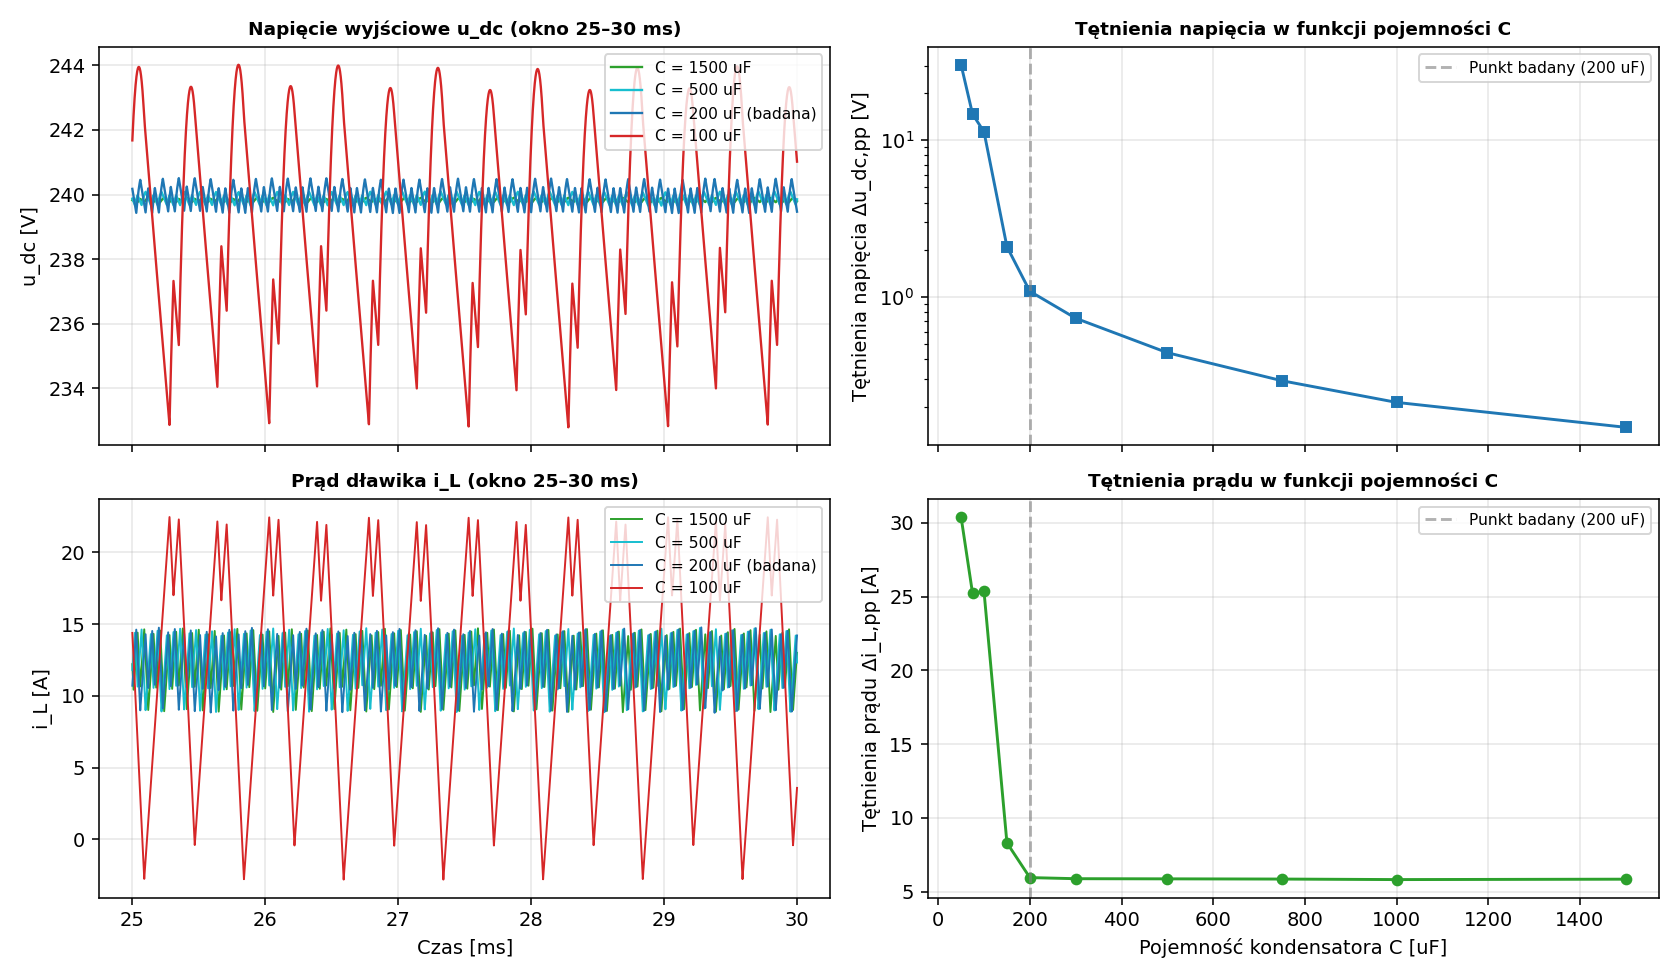
\includegraphics[width=\linewidth]{rysunki/stress_test_pojemnosci_c.png}
    \caption{Badanie zachowania przekształtnika przy redukcji pojemności wyjściowej $C$: (po lewej) przebiegi czasowe napięcia i~prądu w~stanie ustalonym; (po prawej) zależność tętnień napięcia $\Delta u_{\mathrm{dc},\mathrm{pp}}$ oraz tętnień prądu $\Delta i_{L,\mathrm{pp}}$ od pojemności $C$.}
    \label{fig:stress-c}
\end{figure}

Dla pojemności $C \ge 200~\mu\mathrm{F}$ układ zachowuje pełną stabilność, a~tętnienia prądu dławika pozostają na minimalnym poziomie sprzętowym ($\approx 5{,}85$--$5{,}96~\mathrm{A}$). Dla badanej w~pracy pojemności $C = 200~\mu\mathrm{F}$ tętnienia napięcia wynoszą zaledwie $1{,}09~\mathrm{V}$ ($0{,}45\,\%$), co stanowi wynik znakomity. Dopiero zejście poniżej $100~\mu\mathrm{F}$ przy taktowaniu $100~\mathrm{kHz}$ powoduje gwałtowny wzrost tętnień wskutek ograniczeń częstotliwości próbkowania sterownika.

\subsection{Odpowiedź dynamiczna na skoki obciążenia i~referencji}
\label{subsec:transient}

Odporność dynamiczną układu zweryfikowano w~horyzoncie $0{,}30~\mathrm{s}$ w~scenariuszu obejmującym skokowe zrzucenia obciążenia do stanu jałowego ($47{,}619~\Omega \to 10~\mathrm{M}\Omega$ w~$t=50~\mathrm{ms}$ i~$t=200~\mathrm{ms}$), ponowne dołączenia odbiornika $1{,}2~\mathrm{kW}$ ($t=100~\mathrm{ms}$ i~$t=250~\mathrm{ms}$) oraz skok wartości zadanej napięcia $240 \to 160~\mathrm{V}$ ($t=150~\mathrm{ms}$).

We wszystkich stanach przejściowych układ zachował stabilność:
\begin{itemize}
    \item Przy nagłym załączeniu pełnego obciążenia w~$t=100~\mathrm{ms}$ przeregulowanie napięcia wyniosło zaledwie $\Delta U_{\mathrm{overshoot}} = 0{,}51~\mathrm{V}$ ($0{,}21\,\%$ wartości zadanej).
    \item Przy skoku referencji w~dół $240 \to 160~\mathrm{V}$ czas przejścia trwał dokładnie $1{,}3~\mathrm{ms}$, a~napięcie osiągnęło nowy poziom zadany z~naturalnym, łagodnym zapadem $\Delta U_{\mathrm{undershoot}} = 0{,}26~\mathrm{V}$ bez żadnego wtórnego odbicia w~górę.
    \item W~całym horyzoncie $0{,}30~\mathrm{s}$ prąd dławika nie przekroczył poziomu $22{,}63~\mathrm{A}$, co potwierdza skuteczne działanie ogranicznika nadprądowego ($I_{\max} = \pm 20~\mathrm{A}$).
\end{itemize}

\section{Porównanie strojenia AI (PSO) ze strojeniem bazowym}
\label{sec:ai-vs-manual}

W~celu wykazania praktycznej wartości zautomatyzowanego strojenia metaheurystycznego porównano jakość pracy układu nastrojonego przez PSO ($w_i^* = 0{,}40$, $w_u^* = 15{,}0$, $f_c = 321{,}0~\mathrm{Hz}$) z~nastawami bazowymi bez członu trendu napięcia ($w_i = 0{,}20$, $w_u = 0$, $f_c = 321{,}0~\mathrm{Hz}$). Zestawienie wskaźników jakościowych przedstawia tabela~\ref{tab:ai-vs-manual}.

\begin{table}[h!]
    \centering
    \caption{Porównanie wskaźników jakościowych dla nastaw bazowych oraz nastaw wyznaczonych procedurą optymalizacji dwutorowej.}
    \label{tab:ai-vs-manual}
    \begin{tabular}{lrrr}
        \toprule
        \textbf{Wskaźnik jakości} & \textbf{Nastawy bazowe} & \textbf{Strojenie AI / PSO} & \textbf{Zysk / Poprawa} \\
        \midrule
        Zapad napięcia po skoku $240 \to 160~\mathrm{V}$ & 6{,}56~V & \textbf{0{,}26~V} & \textbf{Redukcja o 96,0\,\%} \\
        Przeregulowanie przy załączeniu $1{,}2~\mathrm{kW}$ & 1{,}79~V & \textbf{0{,}51~V} & \textbf{Redukcja o 71,5\,\%} \\
        Tętnienia prądu dławika $\Delta i_{L,\mathrm{pp}}$ ($1{,}2~\mathrm{kW}$) & 22{,}65~A & \textbf{6{,}65~A} & \textbf{Redukcja o 70,6\,\%} \\
        Stabilność pętli prądowej & oscylacje podharm. & \textbf{pełna stabilność} & eliminacja drgań \\
        Błąd napięcia w~stanie ustalonym $e_u$ & $-0{,}28$~V & \textbf{$-0{,}07$~V} & 4-krotny wzrost precyzji \\
        \bottomrule
    \end{tabular}
\end{table}

Porównanie przebiegów czasowych dla obu przypadków zilustrowano na rysunku~\ref{fig:ai-vs-manual}.

\begin{figure}[h!]
    \centering
    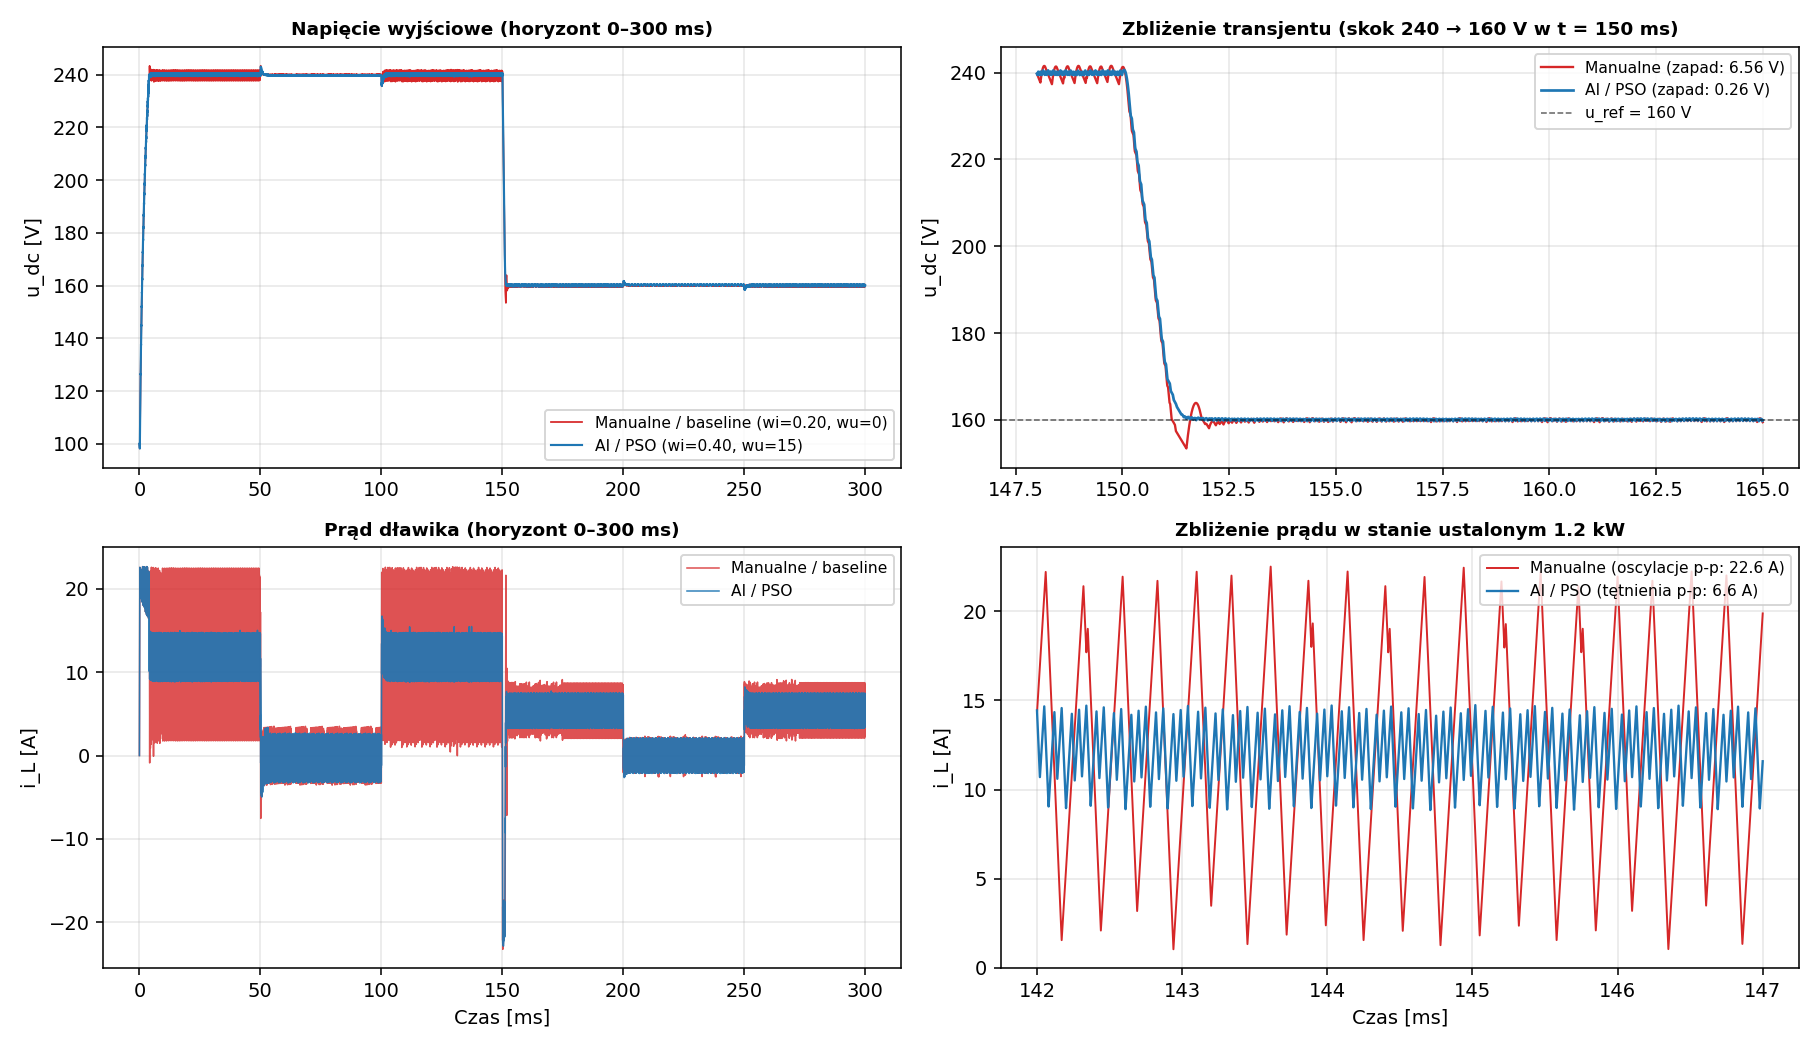
\includegraphics[width=\linewidth]{rysunki/porownanie_ai_vs_manual.png}
    \caption{Porównanie odpowiedzi czasowej przekształtnika: nastawy bazowe (linia czerwona) vs. nastawy nastrojone algorytmem PSO (linia niebieska). Widoczna całkowita eliminacja zapadu napięcia oraz drastyczna redukcja tętnień prądu w~stanie ustalonym.}
    \label{fig:ai-vs-manual}
\end{figure}

Optymalizacja metaheurystyczna przyniosła radykalną poprawę parametrów regulacji: zapad napięcia został zredukowany z~$6{,}56~\mathrm{V}$ do zaledwie $0{,}26~\mathrm{V}$ (poprawa o~$96{,}0\,\%$), a~tętnienia prądu dławika w~stanie ustalonym spadły z~$22{,}65~\mathrm{A}$ do $6{,}65~\mathrm{A}$ (poprawa o~$70{,}6\,\%$) dzięki wyprowadzeniu punktu pracy poza rejon oscylacji podharmonicznych ($w_i > 0{,}25$).

\section{Podsumowanie pracy}
\label{sec:podsumowanie}

\subsection{Realizacja celów pracy}
\label{subsec:realizacja-celow}

Wszystkie cele inżynierskie i~naukowe postawione w~rozdziale~\ref{sec:cel-zakres} zostały w~pełni zrealizowane:
\begin{enumerate}
    \item Opracowano kompletną, obiektową architekturę Bliźniaka Cyfrowego synchronicznego przekształtnika podwyższającego DC-DC w~języku Python, bazującą wyłącznie na bibliotece \texttt{numpy} i~wolną od ciężkich zależności komercyjnych.
    \item Zaimplementowano bezmodelowy algorytm sterowania przełączającego (MF-BB) oraz jego rozszerzenie o~człon trendu napięcia (Trend MF-BB) z~dyskretną filtracją sygnałów metodą Tustina.
    \item Przeprowadzono rygorystyczną walidację symulatora względem oprogramowania PSIM, osiągając zgodność zmiennych stanu na poziomie $0{,}05\,\%$ oraz potwierdzając poprawność równań testem odtworzeniowym (\emph{replay test}).
    \item Zintegrowano silnik symulacyjny z~autorskim algorytmem Optymalizacji Rojem Cząstek (PSO), formułując wielokryterialne funkcje celu uwzględniające jakość napięcia i~tętnienia prądu.
    \item Wdrożono dwutorową procedurę optymalizacji, która wyeliminowała zapady napięcia w~stanach przejściowych przy małej pojemności filtra ($C = 200~\mu\mathrm{F}$) i~wykazano jej wysoką odporność w~systematycznym badaniu wrażliwości.
\end{enumerate}

\subsection{Trudności napotkane podczas realizacji}
\label{subsec:trudnosci}

Podczas realizacji projektu rozwiązano szereg nietrywialnych problemów informatycznych i~symulacyjnych:
\begin{itemize}
    \item \textbf{Opóźnienie próbkowania ZOH i~kolejność zdarzeń:} Osiągnięcie idealnej zgodności z~symulatorem PSIM wymagało zamodelowania jednookresowego opóźnienia przetwornika ADC ($ZOH$ delay) oraz przyjęcia konwencji rejestracji stanu przed wykonaniem kroku fizyki.
    \item \textbf{Pułapka stanu przejściowego w~funkcjach celu:} Naiwne całkowanie błędu prądu na całym horyzoncie czasowym karało sterownik za wymuszone nasycenie prądu podczas rozruchu. Problem rozwiązano poprzez dekompozycję procedury na stan ustalony i~stan przejściowy.
    \item \textbf{Zjawisko fałszywego optimum przy twardej karze za zapad:} Wstępna definicja funkcji celu karząca wyłącznie zapad poniżej wartości zadanej powodowała sztuczne spowalnianie filtru napięcia przez PSO (do $157~\mathrm{Hz}$) kosztem późniejszego odbicia w~górę. Dopiero wprowadzenie kryterium całki kwadratu błędu (ISE) zharmonizowało kompromis pomiędzy szybkością a~gładkością lądowania.
\end{itemize}

\subsection{Wnioski końcowe}
\label{subsec:wnioski}

Przeprowadzone badania pozwalają na sformułowanie następujących wniosków końcowych:
\begin{enumerate}
    \item Standardowy ekosystem języka Python (CPython + NumPy) stanowi w~pełni dojrzałe, wydajne i~precyzyjne środowisko do tworzenia Bliźniaków Cyfrowych układów energoelektronicznych, oferując dokładność całkowicie równoważną dedykowanym narzędziom komercyjnym.
    \item Sterowanie bezmodelowe typu Bang-Bang (MF-BB) w~połączeniu z~członem trendu napięcia wykazuje doskonałe właściwości dynamiczne w~przekształtnikach o~zredukowanej pojemności filtra wyjściowego, skutecznie tłumiąc stany nieustalone.
    \item Dwutorowa optymalizacja metaheurystyczna z~wykorzystaniem algorytmu PSO eliminuje konieczność żmudnego, intuicyjnego strojenia parametrów regulatora, gwarantując powtarzalny dobór nastaw o~udowodnionej odporności na zmiany wag kryteriów optymalizacyjnych.
\end{enumerate}

\subsection{Kierunki dalszych prac}
\label{subsec:przyszlosc}

Naturalnymi kierunkami dalszego rozwoju projektu są:
\begin{itemize}
    \item Zrównoleglenie ewaluacji roju cząstek za pomocą modułu \texttt{multiprocessing} w~celu dalszego skrócenia czasu strojenia na wielordzeniowych stacjach roboczych.
    \item Rozszerzenie modeli symulacyjnych o~nieliniowości elementów pasożytniczych (zależność indukcyjności od prądu nasycenia rdzenia, charakterystyki temperaturowe tranzystorów GaN/SiC).
    \item Eksperymentalna weryfikacja wyznaczonych nastaw regulatora na fizycznym stanowisku laboratoryjnym z~mikrokontrolerem sygnałowym DSP / FPGA.
\end{itemize}


    % Bibliografia - musi być, jest w pliku EE-dyplom.bib
    % Bibliography - must exist, is in the file EE-dyplom.bib
    \bibliografia

    % Strony końcowe - można zakomentować, jeśli zbędne
    % Additional pages - comment out if not needed
    
    % Wykaz symboli i skrótów - patrz opis w tekście przykładowym
    \acronymslist
    % Spis rysunków
    \listoffigures
    % Spis tabel
    \listoftables
    % Załączniki (plik appendices.tex)
    \easyappendices
\end{document}
%%%%%%%%%%%%%%%%%%%%%%%%%%%%%%%%%%%%%%%%%%%%%%%%%%%%%%%%%%%%%%%%%%%%%%%%%%%

